\documentclass[12pt, a4paper]{report}
%\usepackage[a4paper, total={6in, 8in}]{geometry}
\usepackage[utf8]{inputenc}
\usepackage[ngerman]{babel}
\usepackage{color}
\usepackage{comment}
\usepackage{version}
\usepackage[hidelinks, plainpages=false]{hyperref}
\usepackage{graphicx}
\usepackage{longtable}
\usepackage[nohyperlinks, printonlyused]{acronym}
\usepackage{fancyhdr}
%\usepackage[type={CC}, modifier={by-sa},version={4.0}]{doclicense}
\usepackage{listings}
\usepackage[table]{xcolor}
\usepackage{xcolor}
%\usepackage{ccicons}
\usepackage{array,multirow,}
\usepackage{float}
\usepackage{amssymb}
\usepackage{scalerel}
\usepackage{ragged2e}
\usepackage{orcidlink}
\usepackage{pdflscape}
\usepackage{booktabs}
\usepackage{caption} 
\usepackage{appendix}
\usepackage{titlesec}
\usepackage{soul}

\usepackage[babel,german=quotes]{csquotes}
\usepackage[style=numeric, maxbibnames=100,sorting=none, backend=biber]{biblatex}
\usepackage{digsig}
%\usepackage[scaled=0.85]{beramono}
%\usepackage{filecontents}

\titleformat{\chapter}[display]
{\normalfont\bfseries}{}{0pt}{\Huge}

\setcounter{biburllcpenalty}{7000}
\setcounter{biburlucpenalty}{8000}

\labelformat{figure}{Abbildung #1}
\labelformat{table}{Tabelle #1}

\captionsetup[table]{skip=10pt}
\captionsetup[longtable]{skip=10pt}
\captionsetup[figure]{skip=10pt}
\captionsetup[lstlisting]{skip=10pt}

\LTcapwidth=\textwidth

\DeclareFieldFormat{url}{ \url{#1}} % Standard: url: ...
\addbibresource{bibliography/biblio.bib}  
\pagestyle{fancy}
\fancyhf{}
\fancyfoot[C]{\thepage}
\renewcommand{\headrulewidth}{0pt}

\fancypagestyle{firstpage}
{	
	\fancyhf{}
	\chead{ 
\includegraphics[width=\textwidth]{figures/master_bild}}
	\renewcommand{\headrulewidth}{0pt}
}

\renewcommand{\footrulewidth}{0pt}
\setlength\headheight{90.0pt}
%\chead{
\includegraphics[width=\textwidth]{figures/master_bild.png}}

\definecolor{gray}{rgb}{0.4,0.4,0.4}
\definecolor{darkblue}{rgb}{0.0,0.0,0.6}
\definecolor{cyan}{rgb}{0.0,0.6,0.6}

\lstset{
	basicstyle=\ttfamily,
	columns=fullflexible,
	showstringspaces=false,
	commentstyle=\color{gray}\upshape
}

\lstdefinelanguage{XML}
{
	morestring=[b]",
	morestring=[s]{>}{<},
	morecomment=[s]{<?}{?>},
	stringstyle=\color{black},
	identifierstyle=\color{darkblue},
	keywordstyle=\color{cyan},
	morekeywords={xmlns,version,id, value, true, false},
	keepspaces=true,
	basicstyle=\ttfamily\footnotesize, % list your attributes here
}

\definecolor{lightgray}{rgb}{.9,.9,.9}
\definecolor{darkgray}{rgb}{.4,.4,.4}
\definecolor{purple}{rgb}{0.65, 0.12, 0.82}

\lstdefinelanguage{JavaScript}{
	keywords={true, false, id, use, value},
	keywordstyle=\color{blue}\bfseries,
	ndkeywords={class, export, boolean, throw, implements, import, this, id},
	ndkeywordstyle=\color{darkgray}\bfseries,
	identifierstyle=\color{black},
	sensitive=false,
	comment=[l]{//},
	morecomment=[s]{/*}{*/},
	commentstyle=\color{purple}\ttfamily,
	stringstyle=\color{red}\ttfamily,
	morestring=[b]',
	morestring=[b]",
	keepspaces=true,
	basicstyle=\ttfamily\footnotesize, 
}

\definecolor{codegreen}{rgb}{0,0.6,0}
\definecolor{codegray}{rgb}{0.5,0.5,0.5}
\definecolor{codepurple}{rgb}{0.58,0,0.82}
\definecolor{backcolour}{rgb}{0.95,0.95,0.92}

\lstdefinelanguage{SQL}{
	keywords={select, SELECT, where, WHERE, from, FROM, or, OR,  join, and, create, CREATE, view, VIEW, table, on, as, AS, replace, REPLACE, group, by, having, count, order},   
	commentstyle=\color{codegreen},
	keywordstyle=\color{magenta},
	numberstyle=\color{blue},
	stringstyle=\color{codepurple},
	basicstyle=\ttfamily\footnotesize,
	breakatwhitespace=false,
	morestring=[b]',
	morestring=[b]", 
	comment=[l]{--},
	morecomment=[s]{/*}{*/},        
	breaklines=true,                                    
	keepspaces=true,                                     
	numbersep=5pt,                  
	showspaces=false,                
	showstringspaces=false,
	showtabs=false,                  
	tabsize=2
}

\lstdefinelanguage{python}{
	keywords={from, for, with, import, open, as, in, scorer},   
	commentstyle=\color{codegreen},
	keywordstyle=\color{magenta},
	numberstyle=\color{blue},
	stringstyle=\color{codepurple},
	basicstyle=\ttfamily\footnotesize,
	breakatwhitespace=false,
	morestring=[b]',
	morestring=[b]", 
	comment=[l]{\#},
	morecomment=[s]{/*}{*/},        
	breaklines=true,                                    
	keepspaces=true,                                     
	numbersep=5pt,                  
	showspaces=false,                
	showstringspaces=false,
	showtabs=false,                  
	tabsize=2
}

\renewcommand{\lstlistlistingname}{Listingverzeichnis}

\begin{document}
	\pagenumbering{gobble}
	\begin{titlepage}
	\thispagestyle{firstpage}
	\raggedright
	{
		{\normalsize \color{orange} \bfseries BIOMEDIZINISCHE INFORMATIK UND DATA SCIENCE  \\}
		{\normalsize \color{gray} \bfseries Master of Science (M.Sc.)}
		\par
	}
	
	\vspace{1cm}
	
	\centering
	{\scshape\LARGE Masterarbeit \par}
	
	\vspace{1.5cm}
	{\huge \bfseries Wissenschaftliche Nachnutzung der Biosignaldaten aus der Routineversorgung in einem deutschen Universitätsklinikum \par}
	
	\vspace{2cm}
	{\Large Abel \textsc{Hodel\'in Hern\'andez}~\orcidlink{0000-0002-4295-9899}\par}
	\vspace{2cm} 
	betreut von\par
	{Daniel \textsc{Schmitz}\par}

	\vspace{2cm}

	{\large \today\par}
	
	\vfill
	
	
\includegraphics[width=\textwidth]{figures/onder_document}
	
\end{titlepage}
		
	\pagenumbering{Roman}
		
	\tableofcontents	
	\newpage 
	
	\pagenumbering{arabic}
	\begin{abstract}	
	Der Prozess der Digitalisierung im Gesundheitswesen ist ein wichtiger Bestandteil eines sozialen Wandlungsprozesses. Eine der zentralen Herausforderungen in diesem Prozess ist die mangelnde Interoperabilität vieler Systeme, zusammen mit dem gewaltigen generierten Datenvolumen während der Routineversorgung, denn die erfassten Parameter werden nicht immer digital erfasst und werden auch in diversen Systemen gesteuert.
	
	Ziel dieser Arbeit ist die Vorbereitung der in einem \ac{pdms} gespeicherten Biosignaldaten aus der Routineversorgung eines deutschen Universitätsklinikums für die Überführung dieser Bioparameter in einem etablierten Standardformat, nämlich \ac{fhir}; sodass die Interoperabilität der Biosignaldaten gewährleistet wird, und diese Daten in der Zukunft integriert und wieder anwendbar werden können. Dazu werden verschiedene informatische Werkzeuge angewendet, um die gespeicherten Bioparameter mit den Parametern der definierten \ac{fhir}-Spezifikationen zusammenzuführen. Am Ende dieser Zusammenführung entsteht ein Grundgerüst für die zukünftige Überführung der Biosignaldaten in \ac{fhir}.	
\end{abstract}

			
	\chapter{Einleitung} \label{ch:introduction}

Ein wichtiger Bestandteil eines sozialen Wandlungsprozesses ist der Prozess der Digitalisierung im Gesundheitswesen, denn die generierte Datenmenge ist heutzutage nicht im Papierformat zu bewältigen. Dieser Prozess bringt Herausforderungen mit sich, die zu bewältigen sind, sodass die Nutzung moderner \ac{it}-Technologien und Standards im Gesundheitswesen in Bezug auf eine Verbesserung der Versorgung und Forschung im Gesundheitssystem ermöglicht wird. Hinzukommend übt die Digitalisierung auch einen Einfluss auf die Entwicklung der Interaktion zwischen unterschiedlichen an der Gesundheitsversorgung beteiligten Instanzen aus. 

Eine der zentralen Herausforderungen in dem Prozess der Digitalisierung im Gesundheitswesen ist, zusammen mit dem immens generierten Datenvolumen, die mangelnde Interoperabilität vieler Systeme. Denn viele Unternehmen haben eigene Lösungen für einzelne Komponenten herstellt, sodass die Interaktion von Systemen an einem Standort oder die Kommunikation zwischen verschiedenen Standorten in vielen Fällen impraktikabel ist. Eine weitere Problematik der mangelnden Interoperabilität ist die dazu mangelnde Nutzbarkeit der Daten für die Versorgung sowie für die Forschung, die auch die Krankenversorgung in näherer Zukunft fördern könnte. Aus diesem Grund soll innerhalb dieser Masterarbeit der Weg für die Erschließung von Biosignaldaten aus der Routineversorgung an der Universitätsmedizin Mainz primär für die wissenschaftliche Nutzung aufgezeigt werden.
		
	\section{Problemstellung} \label{sec:problem}

In den Krankenhäusern wird eine Unmenge an Daten aus der Routineversorgung gesammelt. Unter diesen Daten befinden sich die Biosignale. Diese sind die Ergebnisse von Messungen oder Beobachtungen. Diese Biosignaldaten werden entweder manuell (Körpergröße, Kopfumfang) oder automatisch durch am Netz verbundene Geräte (Beatmungsdruck, Blutflussindex) erfasst. Die erfassten Parameter werden im Idealfall digital in komplexen Systemen gespeichert. Diese Informationen werden in den meisten Fällen über längere Zeiträume aufgehoben, weil sie entscheidend für die therapeutischen Behandlungen sind. 

Mit der Zeit werden in einem Krankenhaus neue Geräte angeschafft, das Krankenhauspersonal wird erneuert und neue Techniken werden angewendet, sodass bei jeder Erneuerung auch Änderungen in dem System der Speicherung der Daten vorgenommen werden. Außerdem besitzt jedes Krankenhaus seine eigene Systemlandschaft zur Steuerung der Informationen und viele dieser Systeme benutzen keine Standardformate oder Codesysteme bei der Speicherung und Übermittlung der Daten, und somit sind die Daten in den Gesundheitseinrichtungen nicht interoperable. 

Dadurch, dass die Erfassung der Biosignaldaten in den meisten Fällen nicht den etablierten Standards entspricht, könnten solche Daten mit der Zeit unbrauchbar werden oder im schlimmsten Fall verloren gehen. Diese Situation erschwert die Nutzbarkeit der Informationen für die Forschung und Krankenversorgung - nicht nur an einem Standort, sondern auch deutschlandweit.
	\section{Ziel der Arbeit} \label{sec:goal}

Mit der vorher präsentierten Problematik ist das Ziel dieser Arbeit die ersten Schritte zu machen, zur Gewährleistung der Interoperabilität der, für längeren Zeitraum in einem \ac{pdms} an der Universitätsmedizin Mainz, gespeicherten Biosignaldaten, denn diese Information liegt weder in einem Standardformat vor noch beinhaltet es standardisierte gesundheitliche Codesysteme. 

Um dieses Ziel zu erreichen wird die Abbildung der Biosignaldaten des \ac{pdms} in den \ac{fhir}-Spezifikationen des Erweiterungsmoduls \glqq Intensivmedizin\grqq{} des Kerndatensatzes der \ac{mii} erstellt. Die Methode wird an erster Stelle für Forschungszwecke eingesetzt, und sollte die Grundsteine für die Umsetzung und Etablierung des Prozesses am Ende dieses Projekts legen. 

Zusätzlich werden verschiedene \ac{it}-Werkzeuge und Techniken angewendet, um die Biosignalparameter für die spätere Überführung in das Standardformat \ac{fhir} bereitzustellen; sodass diese Daten in der Zukunft nicht nur lokal, sondern auch national und international datenschutzkonform benutzt werden können. 

Hiermit wird, unter anderem, das Versorgungsniveau von Patienten und Patientinnen ausgewertet und zusammen mit anderen Projekten wird die frühzeitige Erkennung von gesundheitlichen Störungen geschaffen \cite{icukdz}.
	\section{Aufbau der Arbeit} \label{sec:structure}

Zu Beginn dieser Arbeit werden zunächst Ansätze und bestimmte Grundlagen zu der zentralen Thematik erläutert. Das Konzept der Interoperabilität insbesondere der Fokus auf dem Gesundheitswesen und die Entwicklung des Kerndatensatzes der \ac{mii} mit verschiedenen Erweiterungsmodulen, wird präsentiert. An dieser Stelle wird sich die Arbeit mit dem Erweiterungsmodul Intensivmedizin befassen. Des Weiteren werden die digitalen Standards für das Gesundheitswesen \ac{hl7} und \ac{fhir} diskutiert. In einer weiteren Sektion werden drei wichtige Codesysteme erläutert. Zusätzlich wird das \ac{pdms} mit Fokus auf das \ac{copra}-System präsentiert. Dazu folgen zwei Sektionen, eine über das Thema \ac{dw}, und die andere behandelt das Data Mapping. Am Ende des ersten Kapitels befasst sich eine Sektion mit dem Thema Pattern Matching und zwei Varianten davon.

In dem Kapitel \glqq Methode\grqq{} wird die Abfolge der Durchführung dieses Projekts dargestellt. Das Kapitel beginnt mit einer kurzen Beschreibung des Prozessablaufes. Des Weiteren folgt die Schilderung der drei behandelnden Schritte des Data Mappings und die Entstehung eines Datensatzes mit zugeordneten Parametern. Anschließend wird die Analyse der Maßeinheiten des Datensatzes und die Rolle der Einheiten für die Programmierung der Transformationsregeln präsentiert. Am Ende wird die Vorbereitung der Überführung der Daten aus \ac{copra} in \ac{fhir} erläutert.

Das Kapitel \glqq Realisierung\grqq{} umfasst die konkrete Durchführung der Methoden zusammen mit Ereignissen, die währenddessen entstanden sind. Anschließend wird die Entwicklung der \ac{db} für die Zwischenspeicherung und Bearbeitung der Daten präsentiert. Zunächst werden in zwei Sektionen die Analyse der Eigenschaften der \ac{fhir}-Profile und die Bearbeitung der Parameter der \ac{fhir}-Profile erläutert. Zwei Sektionen befassen sich mit den Eigenschaften des \ac{copra}-Systems. Danach folgt die Analyse der Parameter beider Systeme diesmal in Zusammenhang mit der Überführung der Biosignaldaten aus \ac{copra} in \ac{fhir}. Zusätzlich wird der Prozess der Zuordnung der \ac{fhir}-Profile mit den Konfigurationsvariablen gezeigt. Eine kurze Sektion präsentiert die Validierung der Zuordnung der \ac{fhir}-Profile mit den Konfigurationsvariablen. Die Durchführung der Analyse der Maßeinheiten und die Behandlung davon für die Programmierung der Transformationsregeln wird weiterhin diskutiert. Die zwei letzten Sektionen befassen sich mit der Bereitstellung der Daten für die Überführung der Biosignaldaten in \ac{fhir}.

In dem Kapitel \glqq Ergebnisse und Diskussion\grqq{} erfolgt eine kritische Bewertung der Projektergebnisse. Die drei Sektionen dieses Kapitels befassen sich mit den Ergebnissen, Nebenergebnissen und Herausforderungen beider angewandten Systeme.

Das Kapitel \glqq Fazit und Ausblick\grqq{} fasst diese Arbeit zusammen und wirft ein Blick auf die mögliche Entwicklung in der Zukunft.
	
	\chapter{Theoretische Grundlagen} \label{ch:theobasis}

Im folgenden Kapitel werden die Grundlagen zu den wichtigsten Konzepten, Fördermaßnahmen und Technologien näher betrachtet, die innerhalb dieser Arbeit im weiteren Verlauf angewendet werden. Zu Beginn wird das Konzept der Interoperabilität und die Erweiterung im Bereich des Gesundheitswesens präsentiert. Die Diskussion der Fördermaßnahme \glqq\ac{mii}\grqq{} mit seinem Kerndatensatz und das Erweiterungsmodul Intensivmedizin folgt im Anschluss. Die \ac{it}-Standards, wie \ac{hl7}-\ac{fhir} und die dazu benutzten Datenaustauschformate, \ac{xml} und \ac{json}, werden nachfolgend erläutert. In einer weiteren Sektion wird sich die Arbeit mit den standardisierten Codesystemen \ac{snomedct}, \ac{loinc} und \ac{ieee} beschäftigen. Das \ac{pdms} und das in Deutschland etablierte Werkzeug \ac{copra} werden präsentiert. Ein Überblick über das \ac{dw}-System wird im weiterem Verlauf der Arbeit verschafft. Anschließend werden Aspekte des Data Mappings und Pattern Matchings in zwei Sektionen erläutert.
	\section{Interoperabilität} \label{sec:interop}

Der Begriff Interoperabilität kann je nach Anwendungsgebiet unterschiedliche Bedeutungen tragen. Die jedoch meist genutzte Definition ist die Folgende: \glqq Fähigkeit von zwei oder mehreren Systemen oder Komponenten, Informationen auszutauschen und die ausgetauschten Informationen wieder zu nutzen.\grqq{} \cite{interopdef}

Diese Definition beinhaltet zwei Ebenen der Interoperabilität, nämlich den Austausch von Information (technische Interoperabilität) und die Nutzung der ausgetauschten Information (semantische Interoperabilität) \cite{telemedizin}. Die dritte Ebene ist die Prozessinteroperabilität \cite{ehealtOk}. Dies wird erreicht, wenn Menschen gemeinsames Verständnis über ein Netzwerk teilen, Systeme zusammenarbeiten und Arbeitsabläufe koordiniert werden \cite{interop}. Im Gesundheitswesen wird auch von der klinischen Interoperabilität gesprochen \cite{ehealtOk}. Diese Ebene ist die Fähigkeit mehrere klinische Fachkräfte in unterschiedlichen Versorgungsteams einzusetzen, um eine nahtlose Versorgung von Patienten und Patientinnen zu gewährleisten \cite{interop}.

\subsection{Interoperabilität im Gesundheitswesen} \label{subsec:interopgesund}

Seit einigen Jahren eröffnet die steigende Vernetzung zusammen mit der Digitalisierung neue Möglichkeiten in der Patientenbetreuung \cite{telemedizin}. Denn es ermöglicht eine neue Art der Kommunikation zwischen dem Personal des Gesundheitssystems an verschiedenen Standorten als auch die Kommunikation mit Patienten und Patientinnen \cite{ehealtOk}. Solche Kommunikation benötigt eine organisatorische und inhaltliche Harmonisierung der zur Verfügung gestellten Daten in Konkordanz mit den neuesten \acsu{it}-Standards und Schnittstellen, um die Interoperabilität zu gewährleisten \cite{telemedizin}. 

Ein wichtiger Aspekt auf dem Weg der Digitalisierung, und somit der Verbesserung des Gesundheitssystems, sind verbindliche Klassifikationen und Ontologien für eine eindeutige und fachliche Kommunikation \cite{ehealtOk}. Diese interoperablen Mittel sollen beim Austausch von Daten und die Implementierung von \ac{it}-Lösungen umgesetzt werden. Um dieses Ziel zu erreichen, wurde in Deutschland im Jahr 2016 vom \ac{bmbf} die \ac{mii} gegründet \cite{telemedizin}. 

Die Aufgabe der \ac{mii} ist die Verbesserung von Forschungsmöglichkeiten und Patientenversorgung durch \acs{it}-Lösungen \cite{mii}. Damit werden Forschung und Versorgung innerhalb und zwischen den Universitätskliniken, Forschungseinrichtungen, Unternehmen, Krankenkassen und Patientenvertreter vernetzt \cite{telemedizin, mii}. In dieser Vernetzung spielen Schnittstellen medizinischer Inhalte mit \acs{hl7} (\ref{sec:hl7fhir}) eine sehr wichtige Rolle für den Austausch der medizinischen Daten \cite{telemedizin}. 

Die Mitglieder der \ac{mii} haben sich auf einen Kerndatensatz (\ref{sec:miikdz}) geeignet, der auf Basis internationaler Standards, wie \ac{snomedct} (\ref{subsec:snomed}), \ac{loinc} (\ref{subsec:loinc}), etc. entwickelt wurde, um die Interoperabilität zwischen den Standorten zu garantieren \cite{telemedizin, miikdz}. Dieser Datensatz beinhaltet zusätzlich verschiedene Erweiterungsmodule für unterschiedliche Use Cases \cite{mii}. Diese Spezifikation ist verbindlich für die syntaktische und semantische Kodierung des Inhaltes der Module \cite{icukdz}.

Das Kernelement der \ac{mii} sind die Datenintegrationszentren (\acsu{diz}s), dessen Herausforderung die Aufnahme, Zusammenführung und Aufbereitung der Daten aus verschiedenen Systemen, sowie die Sicherstellung von Datenqualität und Datenschutz dieser Daten ist \cite{mii, diz}. Damit können die Daten in Versorgung und Forschung genutzt werden. Um dieses Ziel zu erreichen, werden die Daten standardisiert, wiederverwendbar und austauschbar gemacht \cite{diz}. Jedes Mitglied der \ac{mii} besitzt ein lokales \ac{diz}, in dem die lokalen Daten gespeichert werden. Bei verteilten Machbarkeitsabfragen, wie z. B. die Übermittlung der Menge an behandelnden Personen mit einer bestimmten Diagnose, wird die gespeicherte Information datenschutzkonform bereitgestellt, und in aggregierter Form dann zentral bewertet.
	\section{Kerndatensatz der \acs{mii}} \label{sec:miikdz}

Einer der Erfolge der \ac{mii} ist, dass alle Mitglieder der \ac{mii} sich auf einen gemeinsamen Kerndatensatz geeinigt haben \cite{telemedizin, miikdz}. Dieser Datensatz ist die wichtigste Voraussetzung für die zentrale Basis für den gemeinsamen Gebrauch von Daten und, dass dieselbe Auswertungslogik in den \acp{diz} lokal ausgeführt werden kann, denn die Daten in der Patientenversorgung stammen heutzutage aus diversen Quellsystemen und liegen somit in vielen verschiedenen Datenformaten mit unterschiedlichem Inhalt vor \cite{miikdz}. 

Mit diesem Kerndatensatz wurde, unabhängig von Use Case und Indikation der Mitglieder der \ac{mii}, festgelegt, welche Datensätze von den stationären und ambulanten Patienten und Patientinnen die \acp{diz} der \ac{mii} mindestens speichern sollten \cite{miikdz}.

Der \ac{mii}-Kerndatensatz besteht aus Basis- und Erweiterungsmodulen (\ref{fig:mii}). Während die Definition der Basismodule fachlich übergreifend ist, sind die Erweiterungsmodule die Abbildung von Daten spezifischer An- wendungs- oder Fachgebiete, sodass der Kerndatensatz in kontinuierlicher Erweiterung ist \cite{miikdz}.

\clearpage

\begin{figure}[ht]
	\centering
	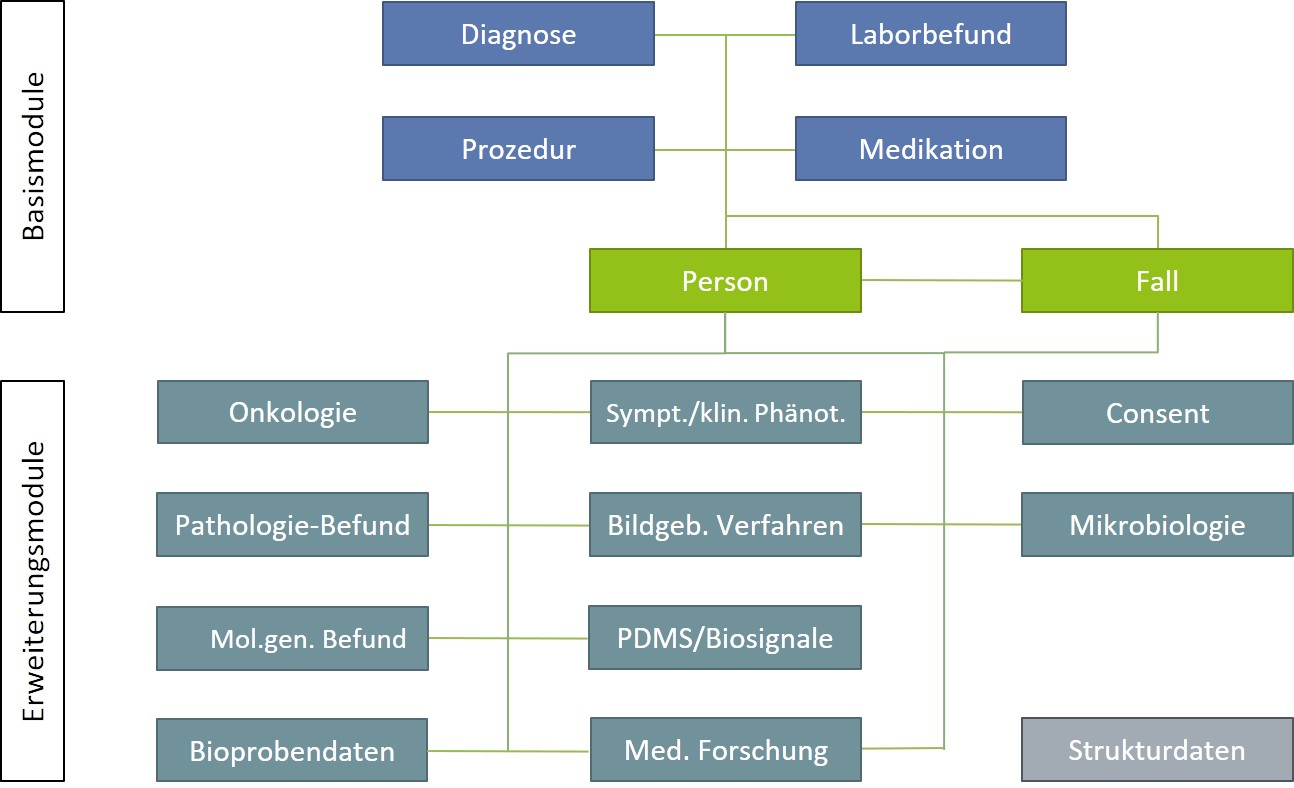
\includegraphics[height=7.5cm]{figures/MIIModule}
	\caption[Kerndatensatz der \acs{mii}]{Kerndatensatz der \acs{mii} und deren Erweiterungsmodule \cite{miikdz}.}
	\label{fig:mii}
\end{figure}

\subsection{Erweiterungsmodul \glqq Intensivmedizin\grqq{} des Kerndatensatzes der \acs{mii}} \label{subsec:icumodul}

Relevant für die Durchführung dieser Masterarbeit ist das Erweiterungsmodul \glqq Intensivmedizin\grqq{} oder \ac{icu}, wie in \ref{fig:mii} als \acs{pdms}/Biosignale genannt. Der Fokus des Projekts liegt ganz konkret auf der \ac{fhir}-Spezifikation des Moduls (\href{https://www.medizininformatik-initiative.de/Kerndatensatz/Modul_Intensivmedizin/IGMIIKDSModulICU.html}{Medizininformatik Initiative - Modul ICU - ImplementationGuide}). Ein wichtiger Hinweis an dieser Stelle ist, dass das Modul \glqq Intensivmedizin\grqq{} auch eine parallele Webseite für die Weiterentwicklung unter der Open Source Plattform SIMPLIFIER.NET (\href{https://simplifier.net/medizininformatikinitiative-modul-intensivmedizin}{Medizininformatik Initiative - Modul ICU}) besitzt, wo die aktuellen Modifikationen veröffentlicht werden. Auf dieser Webseite können die Mitglieder der \ac{mii} und weitere Personen mit Zugang zu dieser Webseite Kommentare und Anmerkungen an die SIMPLIFIER-Webseite des Moduls (\href{https://simplifier.net/MedizininformatikInitiative-Modul-Intensivmedizin/~issues}{Issues}) senden.

Dieses Erweiterungsmodul spezifiziert akutmedizinische Daten für die Primär- und Sekundärnutzung und hat Bezüge zu den Basismodulen (\ref{fig:mii}). Die erste stabile Ballot-Version der \ac{fhir}-Profile des Moduls wurde am 24. Februar 2022 veröffentlicht \cite{modicu}. Ziel der Modellierung dieses Erweiterungsmoduls ist die Datenabbildung der Intensivmedizin und die Darstellung gleichartiger Daten der Notfallmedizin, stationärer und ambulanter Medizin \cite{icukdz}. Ziel des Moduls ist die Unterstützung und Erleichterung der Forschung, Qualitätssicherung, Kommunikation zwischen medizinischen Geräten und der Entscheidungsfindung \cite{modicuvid}.

Das Erweiterungsmodul \glqq Intensivmedizin\grqq{} ist in drei Entwicklungsstufen geplant, davon ist die erste Stufe fertiggestellt, die zweite wurde von 25.02.2022 bis 08.04.2022 zum Abstimmverfahren freigegeben, es ist ein Entwurf zur Korrektur und zum Kommentieren; die dritte Stufe befindet sich immer noch in Entwicklung \cite{modicuvid}.

\begin{enumerate}
	\item Entwicklungsstufe 1: Datenmodell
	\item Datenarten der Entwicklungsstufe 2:
	\begin{itemize}
		\item Monitoring und Vitaldaten
		\item Parameter von extrakorporalen Verfahren
		\item Beatmungswerte
	\end{itemize}
	\item Datenarten der Entwicklungsstufe 3:
	\begin{itemize}
		\item Ein-/Ausfuhrbilanzen
		\item Scores
		\item Hochauflösende Daten
		\item Lagerungstherapie
		\item etc.
	\end{itemize}
\end{enumerate}

 Der Schwerpunkt dieses Projekts liegt in den Parametern der Entwicklungsstufe 2 des Moduls. Obwohl der Abstimmungsprozess dieser Stufe abgeschlossen ist, wurde bis jetzt noch keine neue überarbeitete Version der Entwicklungsstufe 2 fertiggestellt.

 Die Datenarten der Stufe 2 besitzen mindestens ein generisches \ac{fhir}-Profil und viele davon auch ein spezifisches Profil, welches wenn möglich verwendet werden sollte \cite{icukdz, modicuvid}. Die generischen Profile modellieren die Daten unabhängig von einer spezifischen Annotation und beschreiben die Struktur für Gruppen von Elementen einer bestimmten Kategorie und sind somit die ersten in der Baumstruktur der \ac{fhir}-Profile (\ref{fig:icutree}) \cite{icukdz}. Die spezifischen \ac{fhir}-Profile hingegen modellieren zusätzlich eine eindeutige semantische Annotation \cite{modicuvid}.
 
 Unter der Gruppe der Parameter von extrakorporalen Verfahren befinden sich die erfassten Daten von \ac{ecmo}-Maschinen, wie die Dauer einer Hämodialysesitzung. In dieser Gruppe werden die gemessenen und eingestellten Werte zusammen mit dem \ac{ecmo}-Gerät erfasst \cite{icukdz}. 
 
 Die Beatmungswerte der Stufe 2 umfassen Daten, wie die Sauerstofffraktion, das Beatmungsvolumen, etc. Der Aufbau dieser \ac{fhir}-Profile ist analog zu Parametern von extrakorporalen Verfahren \cite{icukdz}.

Die \ac{fhir}-Profile unter der Gruppe Monitoring und Vitaldaten umfassen Daten, wie die Herzfrequenz, Körpergröße, die pulsatilen Blutdrücke (systolisch, mittel und diastolisch), etc. Für die pulsatilen Blutdrücke wurde ein weiteres generisches Profil (Blutdruck Generisch) erstellt, um die Kompatibilität mit den deutschen und internationalen Basisprofilen zu gewährleisten \cite{icukdz}. Diese Profile sind auch eine Zusammensetzung von drei separat kodierten \glqq Observations\grqq{}, die dieselben Attribute teilen, nämlich die Spezifikationen für den systolischen, mittleren und diastolischen Blutdruck \cite{icukdz}.

\begin{figure}[ht]
	\centering
	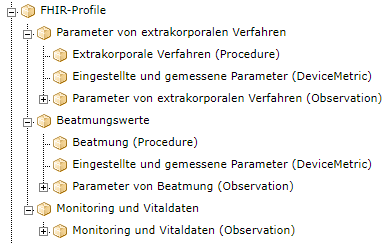
\includegraphics[height=7.5cm]{figures/icu_modul_tree}
	\caption[Baumstruktur des Erweiterungsmoduls \glqq Intensivmedizin\grqq{}]{Baumstruktur des Erweiterungsmoduls \glqq Intensivmedizin\grqq{}.}
	\label{fig:icutree}
\end{figure}

Die semantische Annotation des Erweiterungsmoduls \glqq Intensivmedizin\grqq{} referenziert mindestens einen Primärcode der Terminologie (\ac{snomedct} oder \ac{loinc}) \cite{icukdz, modicuvid}. Um die Interoperabilität mit der Kommunikation zwischen Medizingeräten oder Medizinprodukten zu ermöglichen, wird wenn möglich auch eine semantische Annotation nach \acsu{iso}/\acsu{ieee} 11073-10101\texttrademark{} (\ref{subsec:ieee}) hinzugefügt \cite{icukdz}. Die Maßeinheiten werden nach \ac{ucum} codiert.

\newpage

Die \ac{fhir}-Profile des Moduls \ac{icu} sind in drei Kategorien untergliedert:

\begin{itemize}
	\item DeviceMetric
	\item Observation
	\item Procedure
\end{itemize}

Die \ac{fhir}-Profile der Kategorie \glqq DeviceMetric\grqq{} beschreiben die Messungen und die Einstellungen des benutzten medizinischen Geräts, und sollen wenn möglich mit dem benutzten Gerät verlinkt werden \cite{icukdz}. \glqq DeviceMetric\grqq{}-Profile kategorisieren die Werte in gemessenen und eingestellten Werten \cite{devicemetric}. Die gemessenen Werte sind die während der Untersuchung erhobene Parameter, z. B. die spontane mechanische Atemfrequenz bei der Beatmung. Die eingestellten Werte sind wiederum die Einstellungen an den Geräten, z. B. der eingestellte inspiratorische Gasfluss während der Beatmung.

Die \ac{fhir}-Profile unter der Kategorie \glqq Observation\grqq{} registrieren die Messungen an Patienten, wie Laboruntersuchungen oder die Beobachtungen an Geräten \cite{observation}. Unter dieser Kategorie befinden sich die Vitalparameter.

\glqq Procedure\grqq{}-Profile definieren ein durchgeführtes Verfahren an Patienten, diese können entweder eine physikalische Intervention oder eine Beratung sein \cite{procedure}.

	\section{\acs{hl7} \& \acs{fhir}} \label{sec:hl7fhir}

Wichtig um die Interoperabilität in Gesundheitswesen zu gewährleisten, sind syntaktische \ac{it}-Standards wie \ac{fhir}, der neueste Standard von \ac{hl7} mit Fokus auf den aktuellen Web-Standards und einer einfachen Implementierung \cite{telemedizin, hl7, fhir}.

\subsection{\acs{hl7}} \label{subsec:hl7}

\acf{hl7} ist eine nicht gewinnorientierte, \ac{ansi}-akkreditierte Standardisierungsorganisation zur Bereitstellung eines umfassenden Frameworks und dessen Standards auf der 7. Ebene (Anwendungsschicht) im \ac{iso}/\ac{osi} Modell  
%(\ref{sec:isoosi})
, für den Austausch, die Integration, das Teilen und den Abruf elektronischer Gesundheitsinformationen \cite{telemedizin, ehealtOk, hl7}. \ac{hl7}-Schnittstellen unterstützen die Kommunikation von Softwaresystemen in klinischen Einrichtungen und somit das Management, die Erbringung und Bewertung von Gesundheitsdiensten \cite{ehealtOk, hl7, fhir}.

\subsection{\acs{fhir}} \label{subsec:fhir}

Der \acf{fhir}-Standard eignet sich für den Einsatz in verschiedenen Szenarien, wie den Datenaustausch auf nationaler und internationaler Ebene, in einem regionalen Netzwerk, zwischen Systemen innerhalb einer Organisation und den Datenaustausch mit mobilen Applikationen \cite{ehealtOk, fhir}. 

\ac{fhir} besteht aus drei Bausteinen: Ressourcen (Resources), Referenzen (References) und Profile (Profiles) \cite{fhir}.

In \ac{fhir} werden Konzepte aus der realen Welt als Ressourcen mit entsprechenden für Menschen und Maschinen lesbaren Werten dargestellt \cite{ehealtOk}. Diese wiederum sind logische Einheiten des Datenaustausches mit einem konkreten, definierten Verhalten und eindeutiger Semantik \cite{fhir}. Die Definition der Ressourcen deckt häufig die meisten Anwendungsfälle \cite{ehealtOk}. Jede Ressource besteht aus strukturierten Daten, Narrativen und Ergänzungen (Extensions) \cite{fhir}. Während die strukturierten Daten 80\% der weitverbreiteten Einsatzszenarien abdecken, lassen sich manche Ressourcen durch die Ergänzungen erweitern, die nicht in \ac{fhir} erhältlich sind, um speziellere Anwendungsfälle abdecken zu können \cite{fhir, ehealtOk}. Die Narrative sind dann menschenlesbare Texte, um den Inhalt der Ressourcen zusammenzufassen \cite{fhir}.

Die Referenzen ermöglichen es, dass mehrere Ressourcen und deren Informationseinheiten aufeinander verweisen können, um Beziehungen aufzubauen \cite{fhir}. Ein Beispiel davon sind die \glqq Observation\grqq{}-Ressourcen mit den Werten der Messungen im Erweiterungsmodul \glqq Intensivmedizin\grqq{} verweisen auf die \glqq Patient\grqq{}-Ressourcen mit der Information der behandelnden Personen in dem Basismodul \glqq Person\grqq{} des Kerndatensatzes der \ac{mii} (\ref{fig:mii}).

Viele Werte in den \ac{fhir}-Ressourcen sind optional, sodass eine Umsetzung kompatibel ist, wenn sie nur die minimal obligatorischen Daten liefert. Diese Werte können von außen über die Profile modifiziert werden, und können wiederum sich aufeinander verweisen \cite{ehealtOk}. Das bedeutet die \ac{fhir}-Profile sind die Spezifikationen, die die \ac{fhir}-Ressourcen beschreiben und definieren, z. B. die Festlegung von konkreten Codesystemen \cite{fhir, fhircompact}.

\begin{comment}
Der \ac{fhir}-Standard besitzt fünf Begriffe für die Beschreibung der Stabilität-Ebene \cite{fhircompact}:

\begin{enumerate}
	\item Draft: Dies beschreibt eine nicht komplette oder nicht ausreichende überprüfende Spezifikation. Die Nutzung der Spezifikationen unter dieser Ebene ist riskant.
	\item Trial Use: Solche Spezifikationen sind noch nicht veröffentlicht, trotzdem gut überprüft und von den Autoren für die Nutzung in Systemen empfohlen.
	\item Normative: Diese sind die stabilen veröffentlichten Spezifikationen.
	\item Informative: Diese Spezifikationen definieren keine Regeln und sind für die Assistenz der Implementierung konzipiert.
	\item Deprecated: Die Spezifikationen unter dieser Ebene sind veraltet, und beinhalten Orientierungshilfe für die Anwender und Anwenderinnen. Somit sollen sie verhindern, neue Features in diesen Spezifikationen einzufügen.
\end{enumerate}
\end{comment}

Ein zuvor genannter Aspekt von \ac{fhir} ist seine Fokussierung auf moderne Webprotokolle. Somit können die \ac{fhir}-Ressourcen, die auf einem Server liegen, über eine Schnittstelle via \ac{http} abgefragt werden \cite{telemedizin, ehealtOk}. Außerdem ist das Datenformat für diese Übertragung auch von \ac{fhir} festgelegt, diese kann entweder \ac{xml} oder \ac{json} sein \cite{ehealtOk}. Diese zwei Formate sind weitverbreitet und besitzen eine hohe Akzeptanz durch ihre Versatilität \cite{fhirformat}.

Die \ac{fhir}-Profile können auf verschiedene Art und Weise dargestellt werden. Die am häufigsten benutzten Arten der Darstellung sind logische Tabellen, \ac{xml}- und \ac{json}-Schemata \cite{fhirformat}.

\subsubsection{Logische Tabelle} \label{subsubsec:logtab}

Eine logische Tabelle eines \ac{fhir}-Profils beinhaltet die Spalten: Name, Flags, Card., Type und Description \& Constraints, wobei diese letzte Spalte beim Anklicken eines Elements eingeblendet wird \cite{fhirformat}. \ref{fig:logic-table} zeigt ein Teil der logischen Tabelle eines \ac{fhir}-Profils des Erweiterungsmoduls \glqq Intensivmedizin\grqq{}.

\begin{figure}[ht]
	\centering
	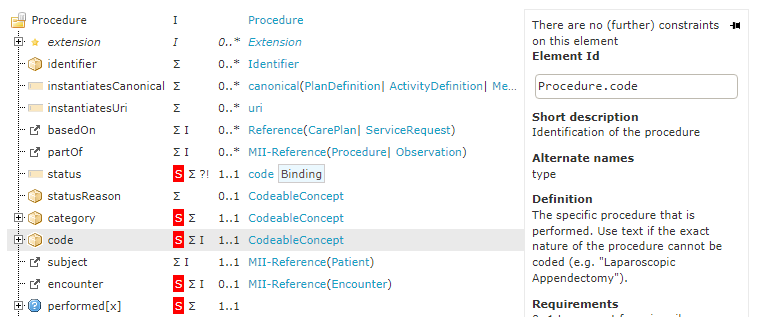
\includegraphics[height=6cm]{figures/beatmung}
	\caption[Logische Tabelle eines \acs{fhir}-Profils]{Fragment der logischen Tabelle des \acs{fhir}-Profils Beatmung des Erweiterungsmoduls \glqq Intensivmedizin\grqq{} des Kerndatensatzes der \acs{mii}.}
	\label{fig:logic-table}
\end{figure}

\begin{itemize}
	\item Name: Name eines Elements in der \ac{fhir}-Ressource. Das Icon bezeichnet den Inhalt des Elements. In der \ref{fig:icons} wird die Bedeutung der Icons erklärt.
	\item Flags: Entscheidende Informationen darüber, wie das Element implementiert werden sollte.
	\begin{itemize}
		\item S: Dieses Element muss unterstützt werden.
		\item I: Elemente mit diesem Symbol definieren Randbedingungen oder sind Teile davon, z. B. das Element \texttt{code} definiert die benutzten Codesysteme bei der \glqq Procedure\grqq{}-Profile (\ref{fig:logic-table})
		\item $\sum$: Diese Elemente sind Teile einer Ressource.
		\item ?!: Das sind modifizierende Elemente, z. B. das Element \texttt{status} beschreibt den Zustand einer \glqq Procedure\grqq{}-Ressource, nämlich \texttt{final}, wenn die Ressource in einer Endversion sich befindet (\ref{fig:logic-table}).
	\end{itemize}
	\item Card.: Cardinality - untere und obere Grenze, wie häufig dieses Element in der Ressource erscheinen darf.
	\item Type: Typ des Elements. Hier erscheint auch der Link zur Definition des Typs.
	\item Description \& Constraints: Beschreibung des Elements und Details über die Einschränkungen.
\end{itemize}

\begin{figure}[ht]
	\centering
	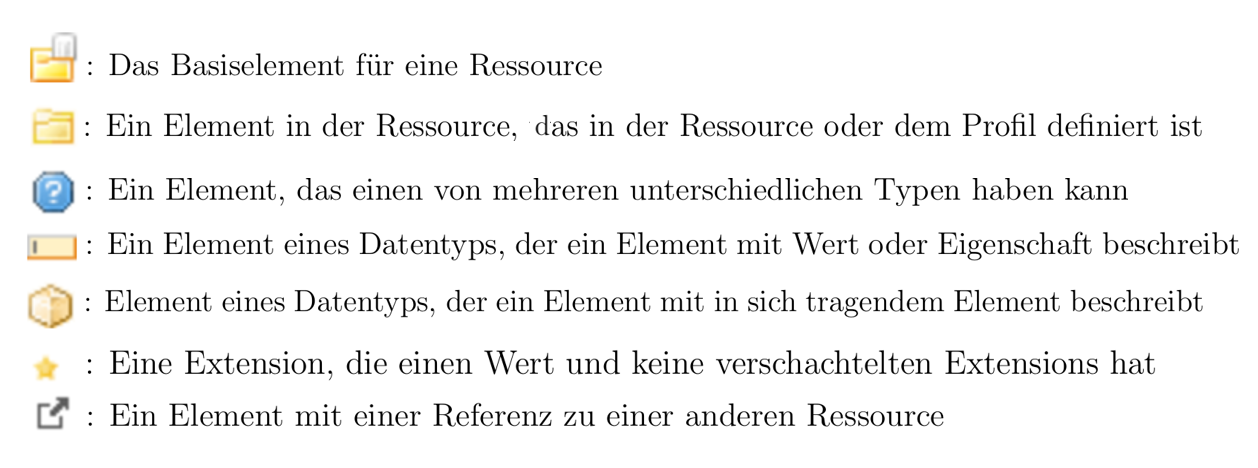
\includegraphics[height=5cm]{figures/icons_description}
	\caption[Beschreibung der meist benutzten \acs{fhir}-Icons]{Beschreibung der meist benutzten \acs{fhir}-Icons.}
	\label{fig:icons}
\end{figure}


\subsubsection{\acs{xml}} \label{subsubsec:xml}

Die Metasprache \acf{xml} hat ihre Wurzeln im Internet und wurde vom \ac{w3c} im Jahr 1998 veröffentlicht und dessen aktuelle Fassung ist die fünfte von 2008 \cite{grundinfo}. Als Metasprache können mit Hilfe von \ac{xml} andere anwendungsspezifische Sprachen, wie \ac{fhir}, definiert werden. Mit \ac{xml} können auch Daten gespeichert oder übertragen werden \cite{interop, grundinfo}.

Ein \ac{xml}-Dokument ist für das Computer-Processing konzipiert, trotzdem kann dieses Dokument von Menschen gelesen werden, denn Dokumente im \ac{xml}-Format sind zur selben Zeit Text-Dateien \cite{grundinfo}. Die Regeln bei \ac{xml}-Dateien sind strikt, sodass Fehler in den Anwendungen verhindert werden. Alle \ac{xml}-Dokumente beinhalten verbundene Knoten in einer Baumstruktur, wo alle Knoten von einer einzelnen Wurzel stammen, das so genannte Element \cite{interop}. Für die Auszeichnung von Elementen werden Tags \glqq $<$, $>$, $/$$>$ \grqq{} verwendet \cite{grundinfo}. Attribute werden in \ac{xml} benutzt, um die Information der Elemente einzufügen \cite{interop, quality}. Der Code \ref{list:xmlpatient} zeigt die \ac{fhir}-\ac{xml}-Datei für die Definition einer Person.

\begin{lstlisting}[caption={[Beispiel einer \acs{fhir}-Ressource in XML] Beispiel einer \acs{fhir}-Ressource für eine Person in XML.},language=xml, label=list:xmlpatient, captionpos=b]
	<?xml version="1.0" encoding="UTF-8"?> 
	
	<Patient xmlns="http://hl7.org/fhir">
	  <id value="xds"/> 
	  <text> 
	    <status value="generated"/>
	  </text> 
	  <identifier> 
	    <use value="usual"/> 
 	    <type> 
	      <coding> 
	        <system value="http://terminology.hl7.org/CodeSystem/v2-0203"/> 
	        <code value="MR"/> 
	      </coding> 
	    </type> 
	    <system value="urn:oid:1.2.3.4.5"/> 
	    <value value="89765a87b"/> 
	  </identifier> 
	  <active value="true"/> 
	  <gender value="male"/> 
	  <birthDate value="1989-05-27"/> 
	  <address> 
	    <postalCode value="55122"/> 
	  </address> 
	  <managingOrganization> 
	    <reference value="Organization/2"/> 
	  </managingOrganization> 
	</Patient>
\end{lstlisting}

Die grundlegende analytische und Design-Aufgabe der Nutzung von \ac{xml} ist die Erstellung von Schemata \cite{grundinfo}. Die Struktur eines \ac{xml}-Dokuments wird in einem Schema beschrieben, das wiederum in \ac{xml} geschrieben ist. Das Schema bestimmt die Struktur eines Dokumenttyps, die für alle Dokumente dieser Art gleich ist \cite{interop, grundinfo}. Es legt die Tags und die Verbindungen zwischen den Elementen fest. Die Schemata werden anhand eines oder mehrerer Schemata mit Hilfe von Anwendungen validiert \cite{grundinfo}. In \ac{hl7} sind zwei Schemasprachen häufig verbreitet, die \ac{xsd} (\ac{xml}-Schemata) des \ac{w3c} zur Strukturdefinition von \ac{xml}-Dokumenten, und Schematron zur Validierung von Inhalt und Struktur von \ac{xml}-Doku- menten \cite{interop}. \ac{xml}-Schemata werden normalerweise als separate Datei mit der Erweiterung .xsd erstellt und über eine Namespace-Deklaration mit der Datei verlinkt \cite{interop}.

\subsubsection{\acs{json}} \label{subsubsec:json}

\acf{json} ist ein, auf Features der Skriptsprache JavaScript basiertes, menschlesbares Datenaustauschformat für die Übertra- gung der Information zwischen Anwendungen \cite{jsondef}. Aus diesem Grund kann die Sprache selbst die Daten in \ac{json}-Format decodieren, und die Daten können als native JavaScript-Objekte direkt angewendet werden \cite{interop}. 

Dadurch dass \ac{json} einfacher als \ac{xml} ist und viele Programmiersprachen schon \ac{json}-Bibliotheken implementiert haben, ist \ac{json} das bevorzugte Datenaustauschformat zwischen Anwendungen im unterschiedlichen Kontext, z. B. \ac{fhir}-Server und Webanwendungen, und damit eine geeignete Option, um Interoperabilität in Gesundheitswesen zu gewährleisten \cite{interop, jsondef}. Der Code \ref{list:jsonpatient} zeigt die \ac{fhir}-\ac{json}-Datei für die Definition einer Person.

\begin{lstlisting}[caption={[Beispiel einer \acs{fhir}-Ressource in JSON] Beispiel einer \acs{fhir}-Ressource für eine Person in JSON.},language=JavaScript, label=list:jsonpatient, captionpos=b]
{
  "resourceType": "Patient",
  "id": "xds",
  "text": 
  {
    "status": "generated",
   },
  "identifier": 
  [
    {
      "use": "usual",
	  "type": {
	  "coding": 
	  [
	    {
	      "system": "http://terminology.hl7.org/CodeSystem/v2-0203",
	      "code": "MR"
	    }
	  ]
	},
	  "system": "urn:oid:1.2.3.4.5",
	  "value": "89765a87b"
	}
  ],
  "active": true,
  "gender": "male",
  "birthDate": "1989-05-27",
  "address": 
  [
    {	  
	  "postalCode": "55122",
	}
  ],
  "managingOrganization": 
  {
    "reference": "Organization/2"
  }
}
\end{lstlisting}

\ac{json} besteht aus sechs Datentypen für die Darstellung von Entitäten der realen Welt \cite{jsondef}:
\begin{enumerate}
	\item String: Unicode-Zeichen
	\item Number: Gleitkomma-Format von JavaScript mit doppelter Genauigkeit
	\item Boolean: Die Werte \texttt{true} und \texttt{false} ohne Anführungszeichen
	\item Null: Leerer Wert
	\item Object: Gruppe von Namens- oder Wertpaaren zwischen $\{$ $\}$
	\item Array: Geordnete Sammlung von Werten
\end{enumerate}
	
	\section{Codesysteme} \label{sec:codesys}

Um die semantische Interoperabilität im Gesundheitswesen zu gewährleisten, werden auch Codesysteme benötigt. Ein Codesystem ist eine organisierte Sammlung von Begriffen, in der jeder Begriff durch mindestens einen intern eindeutigen Code dargestellt wird \cite{bluecodesy}. Weiterhin kann ein Codesystem auch eine sprachabhängige Definition enthalten, wobei einige Konzepte sehr spezifisch sind, andere hingegen können sehr allgemein sein \cite{interop, bluecodesy}.

Codesysteme sind ein wesentlicher Teil bei den medizinischen Anwendungen und den interoperablen Spezifikationen für den Austausch von Daten zwischen Computern \cite{interop}. Außerdem definieren die Codesysteme, welche Symbole oder Ausdrucke existieren und wie sie zu verstehen sind \cite{interop, fhircodesys}.

Manche Codesysteme beinhalten komplexe Ideen mit vielen Subklassifikationen, wie die \ac{icd}, andere wiederum sind weit gefasst, wie \ac{snomedct} (\ref{subsec:snomed}), oder sind auf spezifische Bereiche fokussiert, wie \ac{loinc} (\ref{subsec:loinc}), weiterhin überlappen sich diverse Codesysteme miteinander, wie \ac{icd} und \ac{snomedct} \cite{bluecodesy}.

\subsection{\acsu{snomedct}} \label{subsec:snomed}

Weltweite Standards für Gesundheitsbegriffe werden von der \ac{ihtsdo} bestimmt, weiterhin ist die \ac{ihtsdo} für die Pflege, Weiterentwicklung, Qualitätssicherung und Veröffentlichung des ontologiebasierten Terminologiestandards \ac{snomedct} verantwortlich \cite{snomedofic}. 

\acf{snomedct} ist die umfangreichste mehrsprachige klinische Gesundheitsterminologie, sodass sie in elektronischen Patientenakten verwendet wird \cite{telemedizin, interop}. Darüber hinaus erleichtert die Nutzung von \ac{snomedct} die klinische Dokumentierung und die Berichterstattung \cite{telemedizin}. Außerdem hilft \ac{snomedct} bei der Ermittlung und Analyse von klinischen Daten und darüber hinaus ist \ac{snomedct} sowohl ein Codierschema zur Ermittlung von Begriffen und Konzepten, als auch eine mehrdimensionale Klassifizierung, die es ermöglicht, Konzepte miteinander in Verbindung zu bringen, zu gliedern und nach verschiedenen Kategorien zu analysieren \cite{interop}. 

Das logische Datenmodell von \ac{snomedct} (\ref{fig:snomedmodel}) beinhaltet drei Komponenten: Konzepte (Concepts), Beschreibungen (Descriptions) und Relationen (Relationships), die sich durch \ac{refsets} ergänzen, außerdem sind alle \ac{snomedct}-Komponente durch eine eindeutige numerische Kennung identifizierbar \cite{snomedguide}. 
\begin{itemize}
	\item Die Konzepte repräsentieren medizinische Begriffe und werden hierarchisch von allgemein zu speziell angeordnet.
	\item Die Beschreibungen verknüpfen medizinische Begriffe mit Konzepten. Außerdem beinhaltet ein Konzept eine eindeutige, unmissverständliche Beschreibung dessen Bedeutung und kann auch weitere Beschreibungen erhalten (Synonyme). Dazu enthält jede Übersetzung der \ac{snomedct} eine zusätzliche Menge von Beschreibungen, die Fachbegriffe in anderen Sprachen mit demselben Konzept verlinken.
	\item Die Relationen verknüpfen zwei Konzepte miteinander. Ein Relationstyp oder Attribut wird benutzt, um die Bedeutung der Verbindung zwischen Ausgangskonzept und Zielkonzept zu repräsentieren, weiterhin verbindet der Relationstyp \glqq is-a\grqq{} ein Konzept zu allgemeineren Konzepten und bildet so die Konzepthierarchien in \ac{snomedct}, andere Relationstypen hingegen repräsentieren Aspekte eines Konzepts.
	\item Die \ac{refsets} sind standardisierte \ac{snomedct}-Implementierungen für die Unterstützung von Anforderungen für Anpassungen und Erweiterungen.
\end{itemize}

\begin{figure}[ht]
	\centering
	
\includegraphics[height=3cm]{figures/snomedmodel}
	\caption[\acs{snomedct}-Datenmodell]{\acs{snomedct}-Datenmodell.}
	\label{fig:snomedmodel}
\end{figure}

Die drei \ac{snomedct}-Komponenten des Elements Blutdruck (Blood pressure) werden in der \ref{tab:snomedexample} repräsentiert.

\begin{table}[ht]
	\centering 
	\small 
	\caption[Blutdruck in \acs{snomedct}]{Blutdruck in \acs{snomedct}.}
	\label{tab:snomedexample}
	\begin{tabular}{|p{2.5cm}|p{3.2cm}|p{5.3cm}|}
		\hline 
		 \bfseries Konzept & \bfseries Beschreibung & \bfseries Relation \\ \hline 
		ID: 75367002 - Blood pressure & Blood pressure (observable entity) &  Is a  $\to$  ID: 310611001 - Cardiovascular measure \\ \hline		    
	\end{tabular}
\end{table}

\subsection{\acsu{loinc}} \label{subsec:loinc}

Das \acf{loinc}-System ist seit 1994 eine internationale Zusammenstellung von Begriffen (Terminologie) zur eindeutigen Identifizierung und Kodierung für Laboruntersuchungen, klinische und medizinisch-technische Untersuchungen, medizinische Dokumententypen und Fragebögen/Fragen \cite{loincbfarm, loincpaper}. Somit ermöglicht \ac{loinc} das Zusammenführen von Untersuchungsergebnissen durch standardisierte Bezeichnungen für den Datenaustausch im Gesundheitswesen und die elektronische Kommunikation von Daten zwischen Labor, Klinik und Praxis \cite{interop}. \ac{loinc} erstellt Codes und einen formalen Namen für jedes Konzept, das einer einzelnen Art von Beobachtungsmessung oder Testergebnis entspricht \cite{interop}. Dieser formale \ac{loinc}-Name ist vollständig spezifiziert, sodass er die Merkmale zur erforderlichen Unterscheidung zwischen ähnlichen und unterschiedlichen klinischen Beobachtungen enthält \cite{telemedizin}. \ac{hl7}-\ac{fhir} bietet auch Unterstützung für \ac{loinc} \cite{loincpaper}.

Die \ac{loinc}-\ac{db} stellt einen Satz von eindeutigen Namen und Identifikatoren für die Identifikation von Laboruntersuchungen und weiteren klinischen Testen zur Verfügung \cite{loincbas}. In dieser \ac{db} befinden sich zusammen mit den \ac{loinc}-Coden weitere Parameter, die eine Untersuchung beschreiben, z. B. Maßeinheiten, \glqq Short Name\grqq{} oder Alias und Basis Attribute, sowie der Typ der Untersuchung.

Die Struktur eines \ac{loinc}-Codes beinhaltet heutzutage zwischen drei und sieben Zeichen in der Form \glqq Ziffern-Ziffer\grqq{}. Das \glqq-\grqq{} befindet sich immer an der vorletzten Stelle und die letzte Ziffer des Codes befindet sich zwischen 0 und 9. Diese letzte Zahl ist eine Prüfzahl für den \ac{loinc}-Server, um Fehler bei der Übertragung des Codes zu vermeiden. Diese Menge an Zeichen kann mit dem Wachstum der \ac{loinc}-\ac{db} vergrößert werden \cite{loincoffi}.

Ein \ac{loinc}-Code ist durch sechs Dimensionen in der folgenden Reihenfolge definiert \cite{loincbfarm}: 
\begin{itemize}
	\item Component oder Analyte: Gemessene oder beobachtete Substanz oder Entität
	\item Property: Merkmal oder Attribut der Substanz oder Entität
	\item Time: Zeitintervall, in dem eine Beobachtung gemacht wurde
	\item System: Beobachtetes System (Probenmaterial, Körperteil oder Umgebung)
	\item Scale: Wie der Beobachtungswert quantifiziert oder ausgedrückt wird: quantitativ, ordinal oder nominal
	\item Method: Methode, mit der die Messung oder Beobachtung stattgefunden hat
\end{itemize}

Die Dimension \glqq Method\grqq{} ist operationell und wird nur verwendet, wenn die Technik die klinische Interpretation der Ergebnisse beeinflusst \cite{interop}. Ein Beispiel der \ac{loinc}-Dimensionen ist in der \ref{tab:loincdimensions} dargestellt.

\begin{table}[ht]
	\centering 
	\small 
	\caption[\acs{loinc}-Dimensionen]{\ac{loinc}-Dimensionen des pulmonalvaskulären Widerstandsindexes. \ac{loinc}-Code: \href{https://loinc.org/8834-4/}{8834-4}. ArResis steht für  Resistance/Area\grqq (Widerstand/Fläche), Pt für Point time (Zeitpunkt-Messungen) und Qn für Quantity. Diese Entität besitzt keine Methode, die die Interpretation der Ergebnisse beeinflusst.}
	\label{tab:loincdimensions}
	\begin{tabular}{|p{3cm}|l|l|p{2cm}|l|l|}
		\hline
		\bfseries Component & \bfseries Property & \bfseries Time & \bfseries System & \bfseries Scale & \bfseries Method \\ \hline
		Hemodynamic resistance/Body surface area & ArResis & Pt & Pulmonary vasculature & Qn & - \\ \hline	
	\end{tabular}
\end{table}

\subsection{\acsu{iso}/\acsu{ieee} 11073\texttrademark{}} \label{subsec:ieee}

Das \acf{ieee} ist die weltweit größte technische Fachorganisation, die sich für den Technologiefortschritt zum Nutzen der Bevölkerung einsetzt, und entwickelt somit \acf{iso} Normen, die die Grundlage für viele der heutigen Produkte und Dienstleistungen in der Informationstechnologie darstellen \cite{ieeeiso}. Die verabschiedeten Standards des \ac{ieee} sind häufig die zentrale Quelle für die Standardisierung eines breiten Spektrums aufstrebender Technologien \cite{ieeeglance}. Eine dieser Familien von Standards ist die \acs{iso}/\ac{ieee} 11073\texttrademark{} \cite{ieeeglance, ieeearch}. Diese Serie definiert die Komponente eines Systems, die den Austausch und die Auswertung von Vitaldaten zwischen medizinischen Geräten, zusammen mit der Fernsteuerung solcher Geräte, ermöglichen \cite{ieeearch}. Weiterhin sind diese Standards ein Ansatz, um das Problem der nicht interoperablen Medizinprodukte zu lösen. 

\subsubsection{\acs{iso}/\acs{ieee} 11073-10101\texttrademark{} Nomenklatur} \label{subsub:ieee1107310101}

Die \acs{iso}/\ac{ieee} 11073-10101\texttrademark{} Nomenklatur wurde von dem \acs{iso}/\ac{ieee} 11073\texttrademark{} Standard Komitee der \glqq \ac{ieee} Engineering in Medicine and Biology Society\grqq{} vorbereitet \cite{ieeeiso}. Die \acs{iso}/\ac{ieee} 11073-10101\texttrademark{} Nomenklatur legt Nomenklaturcodes fest, die die Interoperabilität von Medizinprodukten auf semantischer Ebene erleichtern \cite{ieeearch}. Dieser Standard ist auf medizinischen Geräten für die Akutversorgung und Informationen über die Vitalparameter der Patienten und Patientinnen fokussiert \cite{ieeeiso}. Die \acs{iso}/\ac{ieee} 11073-10101\texttrademark{} definiert sowohl die Architektur als auch die Hauptkomponenten der Nomenklatur, zusammen mit ausführlichen Definitionen für jeden konzeptionellen Bereich \cite{ieeesa}. Dieser Standard ermöglicht die Verlinkung mit \ac{loinc} und \ac{snomedct}, außerdem werden auch \ac{fhir}-Extensions entwickelt, die \acs{iso}/\ac{ieee} 11073-10101\texttrademark{} unterstützen \cite{ieeeextending}. Der Abschnitt von \ac{json}-Code \ref{list:jsonieee} zeigt die Anwendung von einem \acs{iso}/\ac{ieee} 11073-10101\texttrademark{}-Identifikator im \ac{fhir}-Profil \glqq Atemzugvolumen-Während-Beatmung\grqq{} des Erweiterungsmoduls \glqq\ac{icu}\grqq{} des Kerndatensatzes der \ac{mii}.

\begin{lstlisting}[caption={[\acs{iso}/\acs{ieee} 11073-10101\texttrademark{} in \acs{fhir}] Beispiel der Anwendung von \acs{iso}/\acs{ieee} 11073-10101\texttrademark{} in \acs{fhir}.},language=JavaScript, label=list:jsonieee, captionpos=b]
{
  "system": "urn:iso:std:iso:11073:10101",
  "code": "151980"
}
\end{lstlisting}

\subsection{\acs{ucum}} \label{sub:ucum}

Der \ac{ucum} ist ein sehr stabiles Codesystem, das alle gegenwärtigen in der internationalen Wissenschaft, Technik und Wirtschaft verwendeten Maßeinheiten umfassen soll \cite{ucumwebnih}. Das Ziel des \ac{ucum} besteht darin, die eindeutige elektronische Übermittlung und Interpretation von Größen zusammen mit ihren Maßeinheiten zu erleichtern \cite{ucumwebnih, ucumweb}. Aus diesem Grund wurde das Codesystem \ac{ucum} bereits von Standardorganisationen wie \ac{hl7} übernommen \cite{ucumweb}.
	\section{\acl{pdms}} \label{sec:pdms}

Das \acf{pdms} unterstützt die klinische Dokumentation auf Intensivstationen \glqq\acf{icu}\grqq{} und hat damit nachweisbare Auswirkungen auf die Vollständigkeit der Patientenakten, den Zeitaufwand für die Dokumentation und die Erhöhung der Patientenqualitätssicherung \cite{pdmsfinanc, pdmsimplem, pdmsicu}. Dieses System umfasst auch Komponenten der computergestützten Auftragserfassung für Ärzte \glqq\ac{cpoe}\grqq{}, denn die Daten aus diesem System sind entscheidend für verschiedene automatisierte Workflows \cite{pdmsfinanc, pdmsicu}. Das \ac{pdms} bietet auch eine spezifische Funktionalität für die Dokumentation der \ac{drg}, welche alle relevanten Daten für die Codierung erfasst \cite{pdmsfinanc, pdmsimplem}.

In Deutschland waren im Jahr 2021 ca. 15 \ac{pdms}-Anbieter bekannt \cite{pdmsgermany}. Unter diesen Anbietern befindet sich der \acf{copra}, welcher an der Universitätsmedizin Mainz und Standort der Realisierung dieses Projekts benutzte \ac{pdms} ist.

\subsection{\acsu{copra}}

\acs{copra} System GmbH ist seit 1993 einer der führenden Anbieter von \acp{pdms} in Deutschland \cite{copradosing, copra}. Dessen Hauptprodukt ist das zertifizierte Medizinprodukt \ac{copra} in der Version 6 \glqq\ac{copra}6\grqq{}. Mit seinen vier Anwendungsgebieten: Ärzte und Ärztinnen, Pflege, Controlling und \ac{it}-Abteilung ist \ac{copra} ein \ac{pdms} für die Dokumentation von Behandlung und Pflege geeignet \cite{copra}. Aus diesem Grund wird \ac{copra} als \ac{pdms} seit 2007 an der Universitätsmedizin Mainz etabliert \cite{copraplaces}.

Für die Ärzte und Ärztinnen bietet das \ac{copra}-System eine transparente und vereinfachte Möglichkeit für die Dokumentation aller relevanten Daten einer Behandlung, denn alle Befunde der behandelnden Personen können in \ac{copra} eingesehen werden, darüber hinaus werden ärztliche Anordnungen dokumentiert und freigeschaltet \cite{copra}.

Mit den sogenannten Arbeitslisten für die Pflege werden die bereits erfolgten und nicht erfolgten Behandlungsschritte in \ac{copra} angezeigt. Außerdem werden die Kurven der Vitalparameter durch die automatische Übernahme von Werten aller an Patienten angeschlossenen Geräte aufgezeichnet. \cite{copra}.

Die Dokumentation der gesammelten Aktivitäten in \ac{copra} werden exportiert, sodass Therapieverfahren und Maßnahmen durch das Controlling ermittelt werden \cite{copra}.

\ac{copra} nutzt etablierte \ac{it}-Technologien, wie Microsoft \acs{sql} Server und .NET Framework, ist skalierbar, virtualisierbar und bietet Freiheiten bei der Gestaltung der Infrastruktur, sodass es für die \ac{it}-Abteilungen attraktiv ist \cite{copra}.

Durch die Freiheiten bei der Gestaltung der Infrastruktur von \ac{copra} ist ein multidimensionales Datenmodell wie in der \ref{fig:copraschema} möglich. 

Das Schema der \ref{fig:copraschema} stellt nur das Datenmodell des Bereichs für die Durchführung dieses Projekts dar, denn das \ac{copra}-System beinhaltet ein Schema mit mehr als 260 Tabellen insgesamt in dem Release 44.0 der Version 1 von 20.10.2015 \cite{copradoc}. Dieses Modell sollte aber nicht mit einem Sternschema in einem \ac{dw} (\ref{subsec:datamodel}) verwechselt werden, denn bei \ac{copra} stellt die Tabelle \texttt{co6\_medic\_data\_patient} mit der Basisinformation der behandelnden Personen, in der \ac{dw}-Theorie (\ref{sec:dw}), eine Dimension dar, und die weiteren Tabellen sammeln Metadaten und die Ergebnisse der Messungen der medizinischen Geräte (Werttabellen), also die Fakten, und beinhalten auch die Hauptschlüssel von \texttt{co6\_medic\_data\_patient} als Fremdschlüssel.

\clearpage

\begin{figure}[ht]
	\centering
	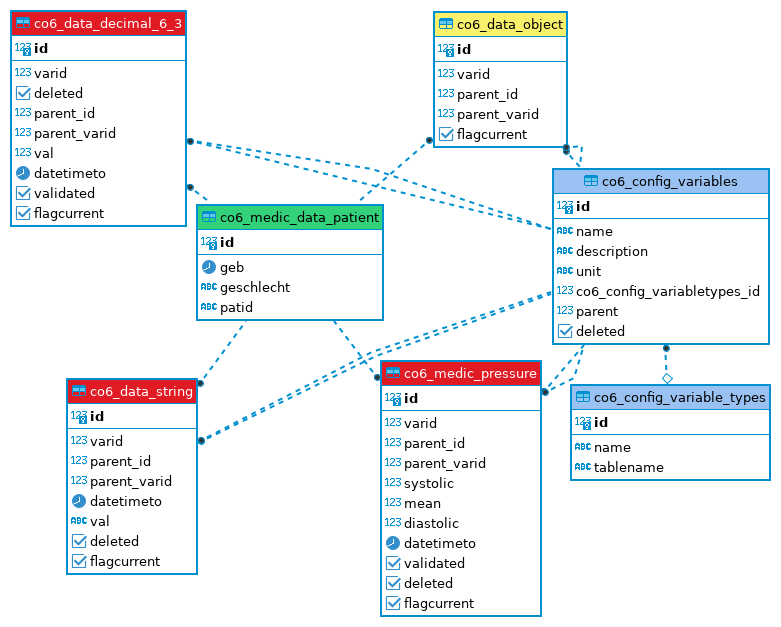
\includegraphics[height=8.5cm]{figures/copra_data_model_data}
	\caption[Datenmodell von \acs{copra}]{Datenmodell des für diese Arbeit benutzten Teils vom \ac{copra}-System an der Universitätsmedizin Mainz. Die Tabelle \texttt{co6\_medic\_data\_patient} beinhaltet die Information der behandelnden Personen. Die Tabellen \texttt{co6\_data\_decimal\_6\_3}, \texttt{co6\_medic\_data\_pressure} und \texttt{co6\_data\_string} speichern die Ergebnisse der Messungen oder Techniken. Die Tabelle \texttt{co6\_data\_object} beinhaltet die Schlüssel aller Objekte, z. B. Patienten und abstrakte Elemente, wie die Arztbriefe oder Scores.
	Die Tabellen \texttt{co6\_config\_variables} und \texttt{co6\_config\_variable\_types} beinhalten die Metadaten der gespeicherten Informationen in \ac{copra}.}
	\label{fig:copraschema}
\end{figure}

Das Teil der \ac{copra}-\ac{db} ist zugleich eine der Datenquelle im Staging Bereich des \ac{dw}  in dem \ac{diz} an der Universitätsmedizin Mainz (\ref{fig:dizummz}).

% Noch dazu stellt dieses benutzte Teil im \ac{copra}-System ein \ac{dm} dar, also ein beschränktes \acf{dw} (\ref{sec:dw}) und somit integriert es Daten aus verschiedenen Datenquellen, in diesem Fall die unterschiedlichen  Messungen und Beobachtungen von den verschiedenen Biosignaldaten, und stellt damit diese Daten zu vielfältigen Analysezwecken zur Verfügung bereit \cite{planungdatawarehouse, dwbauer}. %Damit besitzt \ac{copra} ein \ac{olap}-System (\ref{subsec:olap}) für die Aufbereitung der Daten \cite{planungdatawarehouse, dwbauer}.
	\section{\acl{dw}} \label{sec:dw}

Ein \acf{dw} ist \glqq eine fachlich orientierte, integrierte, nicht volatile und in der Zeit veränderliche Sammlung von Daten zur Unterstützung von Entscheidungen\grqq{} \cite{dworiginal}. Die Eigenschaft der Fachorientierung eines \ac{dw} ermöglicht auch die Nutzung solche Systeme für Forschungszwecke \cite{dwhcliniinv}. Ein \ac{dw} ist auch \glqq eine physische Datenbank, die eine integrierte Sicht auf beliebige Daten zu Analysezwecken ermöglicht\grqq{} \cite{dwgoeken}. Die folgenden Eigenschaften lassen sich aus der Definition ableiten \cite{planungdatawarehouse}.

\begin{itemize}
	\item Fachorientierung: Die Datenstruktur im \ac{dw} wird für die Unterstützung von klinischen Problemstellungen und Entscheidungen optimiert und somit für die Berechnung von Kennzahlen und deren Zuordnung
	\item Integration: Daten aus diversen Datenquellen werden in getrennte \acp{db} integriert, z. B. die Informationen der verschiedenen Quellsysteme in einem Krankenhaus werden in unterschiedlichen \acp{db} des Staging Bereichs eines \ac{dw} gesammelt
	\item Beständigkeit: Die geladenen Daten im \ac{dw} bleiben unverändert
	\item Historisierung: Die über lange Zeit gespeicherten Daten ermöglichen die Erkennung von Entwicklungen und Trends in den Daten
\end{itemize}

Die Anwendungsbereiche von \acp{dw} in klinischen Einrichtungen umfasst die Bereitstellung von Informationen, komplexe und flexible Datenanalyse, die Entwicklung von Forschungsprojekten und die Unterstützung der Planungsprozesse \cite{planungdatawarehouse}.

Die Architektur eines \ac{dw} besteht aus fünf Ebenen \cite{dwbauer}. Die Ebene der Datenquellen umfasst die internen und externen Datenquellen mit relevanten Daten \cite{dwgoeken}. In der Datenerfassungsebene werden diese Daten mit Hilfe von \ac{etl}-Prozessen (\ref{subsec:etl}) für das Laden in die zentrale \ac{db}-System (Datenhaltungsebene) extrahiert, aufbereitet und konvertiert \cite{dworiginal}. Diese zentrale \ac{db} ist in mehreren \acp{db} ausgeteilt, und jede davon stellt eine bestimmte Datenquelle dar \cite{dwgoeken}. In der Datenbereitstellungsebene werden die gespeicherten Daten für multidimensionale Analysen aufbereitet \cite{dwbauer}. Auf der Präsentationsebene befinden sich Anwendungsprogramme mit Zugriff auf die aufbereiteten Daten für die Analyse \cite{dwtool}.

\subsection{\acs{etl}} \label{subsec:etl} 

Die \acf{etl}-Prozesse oder Erfassungsprozesse in einem \ac{dw} dienen der Aufbereitung und dem Laden der Daten in die \acp{db} des \ac{dw}. Diese Prozesse sind je nach Datenmenge und Design des \ac{dw} sehr zeitintensiv \cite{dwbauer, dwtool}.

Zuerst werden bei der Datenextraktion die Daten aus den verschiedenen Datenquellen extrahiert und in einen Zwischenspeicher übertragen, dem sogenannten Staging Bereich \cite{dwtool}. In diesem Prozess werden die ersten Umwandlungen, wie die Pseudonymisierung von personenbezogenen Daten und die Konvertierung von Datentypen zwischen dem Quellsystem und dem \ac{dw}, vorgenommen \cite{dwbauer}.

Nach der Datenextraktion werden die Daten transformiert. Ziel der Transformation ist eine hohe Qualität der Daten zu gewährleisten. Damit werden die extrahierten Daten bereinigt, harmonisiert und zusammengeführt. Bei der Transformation werden Fehler und Inkonsistenzen beseitigt. Ein weiterer Aspekt der Datentransformation ist die Erstellung von Metadaten und künstlichen Schlüsseln zur Erleichterung der Referenzen auf die Datensätze im \ac{dw}, denn in manchen Fällen werden die Schlüssel der Quellsysteme nicht verwendet, denn zwei oder mehrere Quellsystemen können dasselbe Schlüsselschema haben \cite{dwbauer, dwtool}, z. B. die Nutzung von fortlaufenden Nummern als Primärschlüssel für die Identifikation von Diagnosen in verschiedenen Datenquellen.

Die Ladephase ist die Letzte im \ac{etl}-Prozess. Damit werden die transformierten Daten physikalisch in die Zieltabellen des \ac{dw} überführt \cite{dwgoeken, dwtool}.

Ein Beispiel eines \ac{etl}-Prozesses ist in der \ref{fig:dizummz} im Kapitel \glqq Realisierung\grqq{} (\ref{ch:results}) dieses Projekts dargestellt.

\subsection{Datenmodell eines \acs{dw}} \label{subsec:datamodel}

Das Datenmodell eines \ac{dw} orientiert sich an Sachverhalten eines Unternehmens, und somit ist ein \ac{dw} themenorientiert und bietet eine aggregierte Sicht auf das Geschehen \cite{dwgoeken}.

Das Datenmodell eines \ac{dw} ist multidimensional und somit weit verbreitet für die Darstellung analytischer Daten, außerdem ist dieses Modell relativ einfach und vereinfacht die Modellierung der physikalischen \ac{db} eines \ac{dw} \cite{dwbauer}. Andere Vorteile dieser Modellierungsart sind die Performanz und die verständliche Darstellung der Daten für wissenschaftliche Fragestellungen \cite{dwtool}.

Das multidimensionale Modell besteht aus Dimensionen und Fakten \cite{dworiginal}. Die Dimensionen (Dimensionstabellen) sind Konzepte oder Hierarchien, um die Daten zu kategorisieren. Die Fakten (Faktentabellen) sind Beobachtungen, Berechnungen oder Messungen \cite{dwtool}. Der Hauptschlüssel der Faktentabellen ist meist ein künstlicher Schlüssel, der die Kombination der Hauptschlüssel der Dimensionstabellen enthält \cite{dwbauer, dwtool}. 

Die Daten in einem multidimensionalen Datenmodell werden in einer physikalischen \ac{db} eines \ac{rdms}, wie PostgreSQL oder Microsoft SQL Server, meist in einem Sternschema gespeichert und dargestellt \cite{dworiginal}. Seinen Namen verdankt das Schema seiner Ähnlichkeit mit einem Stern, wie in der \ref{fig:starschema} dargestellt wird \cite{dwtool}.

\clearpage

\begin{figure}[ht]
	\centering
	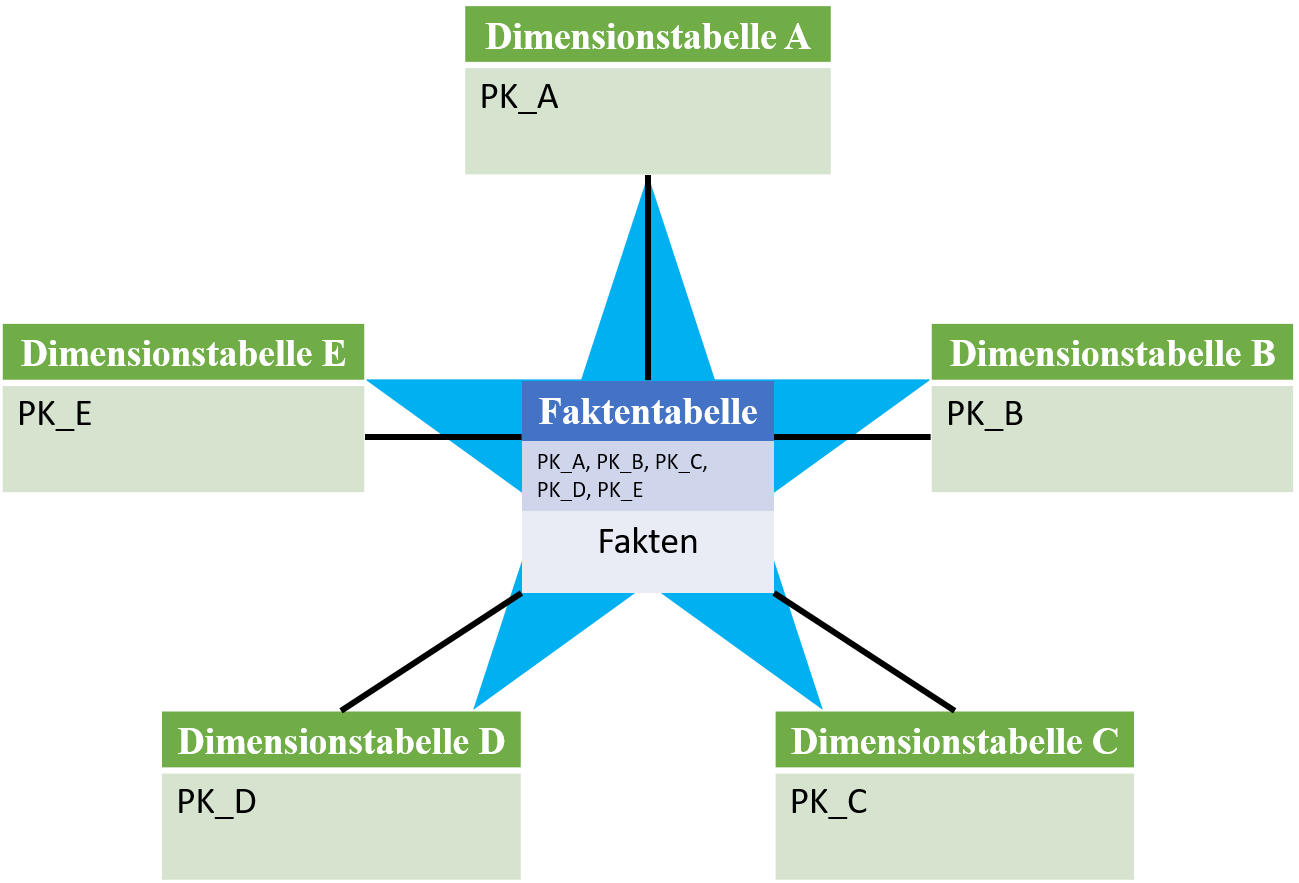
\includegraphics[height=8.5cm]{figures/starschema}
	\caption[Sternschema]{Sternschema. Die Dimensionstabellen beinhalten Kategorien. Die Faktentabelle beinhaltet die Hauptschlüssel der Dimensionstabellen und die Ergebnisse von Analysen. \glqq PK\_\grqq{} stellt die Hauptschlüssel der Tabellen dar.}
	\label{fig:starschema}
\end{figure}

	\section{Data Mapping} \label{subsec:tbasub}

Data Mapping oder Datenzuordnung ist die Herstellung der Verbindung zwischen den Attributen zweier unterschiedlicher Datenmodelle (Quelle und Ziel) \cite{datamappingqs}. Dieses Verfahren wird angewendet, um unterschiedliche Datenquellen zu integrieren und sinnvoll zu nutzen \cite{datamappingastera}. Die Datenzuordnung ist entscheidend für weitere Schritte in Projekten bei denen zwei oder mehrere Datenmodelle eine Rolle spielen \cite{datamappingqs}. Das Ziel der Datenzuordnung ist die Gewährleistung des Transports von Informationen von der Quelle zum Ziel mit so wenig Datenverlust wie möglich \cite{datamappingastera}. Für den Erfolg des Data Mappings sollte man genau wissen, wie die Daten vom Quellsystem zum Zielsystem fließen \cite{datamappingqs}. 

In der Gesundheitsbranche hilft die Datenzuordnung durch das Abgleichen von Daten zwischen Quell- und Zielsystemen die Interoperabilität für die \aclu{ehr} zu erreichen \cite{interop, datamappingastera}. Allerdings hilft die Datenzuordnung auch dem medizinischen Personal, Informationen der behandelten Personen auszutauschen und Gesundheitsdaten aus den verschiedenen Datenquellen zu kombinieren \cite{datamappingastera}.

Dadurch dass der Staging Bereich eines \ac{dw} der Zwischenspeicher ist, in dem die Daten aus den Quellsystemen für die spätere Transformationen gelagert werden, ist dieser Bereich sehr entscheidend für die Datenzuordnung, weil das Data Mapping die inhaltliche Information und Datenstruktur verschiedener Tabellen aus dem Quellsystem benötigt \cite{datamappingqs, datawarehouse}.

Für die Durchführung eines Data Mappings sind drei Elemente entscheidend: das \ac{ldm}, das \ac{pdm} und die fachlichen Spezialisten \cite{datamappingqs}. Einerseits liefert das \ac{ldm} die Details der Strukturdefinition der Datenquelle \cite{datamappingqs, datamodel}. Andererseits beschreibt das \ac{pdm} die Spezifikationen der Implementierung des \ac{ldm} \cite{datamodel}. Die fachlichen Spezialisten besitzen das Fachwissen über eine bestimmte Thematik und stehen somit bei Fragen und Problemen zur Verfügung \cite{smeitlexicon}.

Es gibt drei Data Mapping-Haupttechniken \cite{datamappingastera}:
\begin{enumerate}
  \item Manuelle Datenzuordnung: Manuelle Kodierung der Datenquellen oder manuelle Zuordnung des Zielschemas
  \item Schemazuordnung: Halbautomatischer Prozess bei dem eine Beziehung zwischen Quell- und Zielschema hergestellt wird und die Verbindungen geprüft und gegebenenfalls angepasst werden
  \item Vollautomatische Datenzuordnung: Diese Technik bietet eine bequeme, einfache und effiziente, meist codefreie, Benutzeroberfläche
\end{enumerate}

Das Data Mapping wird in verschiedenen Szenarien angewendet. Eines davon ist, wie bei diesem Projekt, der elektronische Datenaustausch von Gesundheitsdaten, bei dem die Quelldaten in verschiedene Formate konvertiert werden sollen \cite{datamappingastera}.

Das Data Mapping besteht aus sechs Schritten \cite{datamappingtalend}. 
\begin{enumerate}
  \item Definition der Daten für die Verschiebung - Tabellen, Felder und Datenformat der Felder werden definiert
  \item Zuweisung der Quell- und Zielfelder
  \item Transformation - Programmierung der Transformationsregeln
  \item Test - Test mit Beispieldaten aus der Quelle, um mögliche Anpassungen vorzunehmen
  \item Implementierung 
  \item Migration oder Integration der Daten
\end{enumerate}

In dieser Masterarbeit werden zum Teil einige Transformationsregeln definiert, und programmiert.

Dadurch, dass Data Mapping eine dynamische Schnittstelle ist, sollte es regelmäßig gewartet und aktualisiert werden \cite{datamappingtalend}.

Dieses Projekt befasst sich mit dem manuellen Data Mapping für den Datenaustausch von Biosignaldaten aus der \ac{copra}-Instanz des Staging Bereichs eines \ac{dw}, als Quellsystem, zu einem Zielsystem in \ac{fhir}. Das manuelle Data Mapping wurde ausgewählt, denn bis jetzt existieren noch keine vorherigen Projekte - weder an der Universitätsmedizin Mainz noch an anderen \ac{mii} Standorte, welche sich mit dem Data Mapping von Biosignaldaten aus \ac{copra} mit \ac{fhir}-Profilen befassen.
	\section{Pattern Matching} \label{subsec:pattmatch}

Bei der String Suche oder dem Pattern Matching ist das Problem, alle Elemente einer Zeichenkette \texttt{x} der Länge \texttt{p} (Pattern) in einer anderen Zeichenkette \texttt{t} (Text) der Länge \texttt{n} zu lokalisieren \cite{patternmatchingapostolico}. Eine weitere hilfreiche Definition, um das Pattern Matching in der Praktik zu verstehen, ist die Bezeichnung \glqq Teilwort\grqq{}. \glqq Ein Wort \texttt{T} heißt Teilwort des Wortes \texttt{W}, wenn es Worte \texttt{U, V} gibt, so dass gilt: \texttt{W} = \texttt{UTV}\grqq{} \cite{teilwort}. Genau gesagt, ist das Pattern Matching der Prozess ein Teilwort eines Wortes zu erkennen.

Das Pattern Matching wird in verschiedenen Szenarien verwendet \cite{patternmatchingapps}. Einige der Anwendungsbereiche sind Texteditoren in Computern für die Syntaxprüfung von Sprachen oder Rechtschreibprüfung, Programmierung von Datenbankabfragen, in der Bioinformatik für den Abgleich von DNA- oder Eiweißsequenzen, Entwicklung von Systemen zur Erkennung von Eindringlingen in Netzwerke, digitale Bibliotheken, Suchmaschinen und viele weitere Anwendungen \cite{patternmatchingapps, patternmatchingeffi, regexconf}.

Einige der Methoden um Zeichenketten oder Muster zu finden sind die unscharfe Suche (fuzzy search) (\ref{sub:levdist}) und die Anwendung von \acp{regex} (\ref{sec:regex}).

Manche Programmiersprachen, wie Python und \ac{rdms}, wie PostgreSQL, besitzen Features für die unscharfe Suche und \acp{regex}, um einen Text nach Mustern zu durchsuchen \cite{ patternmatchingpostgres, thefuzzlib}.

\subsection{Unscharfe Suche} \label{sub:levdist}

Bei der unscharfen Suche, fuzzy-Suche oder fuzzy search wird eine Ähnlichkeit-Funktion benutzt. Diese Funktion bildet ein Paar Zeichenfolgen \texttt{s} und \texttt{t} auf eine reelle Zahl \texttt{r} ab, wobei ein größerer Wert von \texttt{r} eine größere Ähnlichkeit zwischen \texttt{s} und \texttt{t} anzeigt \cite{stringsearch2}. Eine der bekannten Funktionen ist die \glqq Levenshtein distance\grqq{}. Diese Funktion stellt die Kosten für die Transformation eines Strings in einem anderen dar. Die erlaubten Operationen für die Transformationen sind die Einführung neuer Zeichen, das Löschen und die Substitution von Zeichen \cite{stringsearch2}. Eine Variante der \glqq Levenshtein distance\grqq{} betrachtet auch die Transposition von Zeichen \cite{thefuzzyalgo}.

\subsection{\acs{regex}} \label{sec:regex}

Die \acfp{regex} oder reguläre Ausdrücke sind eine Art Sprache, die in der Informatik für diverse Zwecke angewendet werden kann, insbesondere bei der Bearbeitung von Texten oder bei der Suche von bestimmten Mustern in einem Text \cite{regexconf}. Ein regulärer Ausdruck wird als eine Expression definiert, die eine Menge von Zeichenketten \glqq reguläre Sprache\grqq{} oder eine Menge von geordneten Paaren von Zeichenketten \glqq reguläre Beziehung\grqq{} beschreibt \cite{regexhandbook}. Sie sind in einer Vielzahl von Programmiersprachen und \ac{it}-Anwendungen verfügbar. Ein \ac{regex} wird mit einem Muster von Symbolen erstellt, das sogenannte Metazeichen, die zur Definition des Musters dienen und auch syntaktische Regeln besitzen \cite{regexweb1}.

\begin{itemize}
	\item \textbackslash d: Platzhalter für eine Ziffer, z. B. 5
	\item \textbackslash w: Platzhalter für ein alphanumerisches Zeichen oder Unterstrich \glqq\_\grqq{}, z. B. G
	\item \textbackslash W: Platzhalter für ein Zeichen, dass keine alphanumerisches Zeichen oder Unterstrich ist, z. B. ?
	\item $[...]$: Definiert ein Set von Zeichen, z. B.  [acd]
	\item $\vert$:  Trennung von zwei oder mehreren Alternativen, z. B. x $\vert$ y
	\item +: Mindestens einmal
	\item \{n\}: Genau \texttt{n}-mal
	\item \{min, max\}: Mindestens \texttt{min}-mal und maximal \texttt{max}-mal	
	\item \{min, \}: Mindestens \texttt{min}-mal
	\item \{, max\}: Maximal \texttt{max}-mal
	\item (...): Gruppierung
\end{itemize}

Das folgende Beispiel zeigt der Definition eines \ac{regex} für die Erkennung von Zeichenketten, wie die Maßeinheiten cm[Hg] oder mm[H2O]. Der \ac{regex} \glqq[cm]m\textbackslash WH(g$\vert$2O)\textbackslash W\grqq{} definiert eine Zeichenkette mit \glqq c\grqq{} oder \glqq m\grqq{} gefolgt von \glqq m\grqq{}. Nach diesem Charakter muss ein nicht alphanumerisches Zeichen platziert werden, dieses ist von einem \glqq H\grqq{} und einer Gruppe von Charakteren mit entweder \glqq g\grqq{} oder \glqq 2O\grqq{} gefolgt. Nach der Gruppierung muss sich ein nicht-alphanumerisches Zeichen befinden.
	
	\chapter{Methode} \label{ch:methods}

Um das Ziel dieses Projekts zu erreichen, werden die in dem \ac{pdms} der Universitätsmedizin Mainz gespeicherten Biosignaldaten zu den \ac{fhir}-Profilen des Erweiterungsmoduls \glqq Intensivmedizin\grqq{} des Kerndatensatzes der \ac{mii} zugeordnet und für die Überführung in \ac{fhir}-Ressourcen bereitgestellt. Dazu werden etablierte \ac{it}-Werkzeuge, wie \ac{sql}, Data Mapping, Pattern Matching und \ac{etl}-Prozesse angewendet.

Für die Durchführung dieses Projekts an der Universitätsmedizin Mainz werden die Parameter der \ac{fhir}-Profile des Erweiterungsmoduls \ac{icu} zusammen mit den, in der \ac{copra}-Instanz des Staging Bereichs des \ac{dw} des \ac{diz}, gespeicherten Konfigurationsvariablen in eine \ac{db} importiert. Diese Variablen stellen unter anderem die Messungen und Beobachtungen der Bioparameter dar. In dieser \ac{db} werden die notwendigen Schritte für die Zuordnung der Konfigurationsvariablen mit den \ac{fhir}-Profilen durchgeführt. 

Nach dieser Zuordnung wird der resultierende validierte Datensatz in der \ac{copra}-Instanz des Staging Bereichs des \ac{dw} für die Bereitstellung der Daten für die Implementierung und Automatisierung des Prozesses des Exports der Biosignaldaten in \ac{fhir}-Ressourcen gespeichert.
	\section{Schritte für die Durchführung} \label{sec:steps}

Für die Umsetzung dieser Arbeit wird eine \ac{db} in PostgreSQL entwickelt, um die Information der \ac{fhir}-Profile und Konfigurationsparameter der \ac{copra}-Instanz des Staging Bereichs des \ac{dw} des \ac{diz} an der Universitätsmedizin Mainz zu speichern, und einige der Schritte des Data Mappings durchzuführen.

Die \ac{fhir}-Profile des Erweiterungsmoduls \glqq\ac{icu}\grqq{} werden analysiert, und die allgemeinen Parameter der Profile werden in der entwickelten \ac{db} gespeichert. Einige dieser Parameter werden als Hilfsmittel für die Datenzuordnung angewendet. Andere hingegen spiegeln die Attribute der Biosignaldaten in \ac{copra} wider.

Nach der Speicherung der Profile wird die Struktur der Tabellen von \ac{copra} in dem Staging Bereich des \ac{dw} analysiert. Diese beinhalten die Konfigurationsvariablen und die Werte der Biosignaldaten mit den Attributen für das Data Mapping mit den \ac{fhir}-Profilen. 

Die Voraussetzungen für die Auswahl der Konfigurationsvariablen für die weitere Durchführung des Projekts werden definiert, nämlich patienten- oder fallbezogene Variablen, mit mindestens 1000 validierten, aktuellen und nicht gelöschten Datensätzen in den Werttabellen (\ref{subsec:datadef}).

Nach der Auswahl werden die entscheidenden Attribute der Konfigurationsvariablen in die vorher entwickelten PostgreSQL \ac{db} importiert. Diese Konfigurationsvariablen beinhalten die Namen von Beobachtungen und Messungen, also die \glqq Procedure\grqq{}- und \glqq Observations\grqq{}-Profile.

Mit den gespeicherten Informationen der \ac{fhir}-Profile und den Konfigurationsvariablen in der \ac{db} und der analysierten Datenstruktur von \ac{copra} wird das manuelle Data Mapping durchgeführt. Von diesem Prozess werden in diesem Projekt drei Schritte umgesetzt, nämlich die Datendefinition, Zuweisung der Quell- und Zielfelder, und die Programmierung der Transformationsregeln.

Der Prozess für die Verlinkung der Konfigurationsvariablen mit den \ac{fhir}-Profilen generiert einen Datensatz mit den notwendigen Attributen der Konfigurationsvariablen und der \ac{fhir}-Profile. Dieser Datensatz wird validiert, und die Maßeinheiten beider Systeme werden verglichen, um Fehler und andere Irregularitäten zu detektieren, und wenn möglich, mit der Kooperation der fachlichen Spezialisten der \ac{pdms}-Abteilung und Transformationsregeln solche Probleme zu lösen. Diese Regeln werden in dem Datensatz der zugeordneten Konfigurationsvariablen mit den \ac{fhir}-Profilen eingefügt.

Der Datensatz der zugeordneten Konfigurationsvariablen mit den \ac{fhir}-Profilen wird danach in die \ac{copra}-Instanz des Staging Bereichs des \ac{dw} angelegt, um 
%die Überführung der Biosignaldaten aus \acs{copra} in den \ac{fhir}-Profile einzuplanen, und
 weitere Transformationsregeln für die Erzeugung der \ac{fhir}-Ressourcen aus den Biosignaldaten von \ac{copra} zu definieren.

Mit dem Datensatz der zugeordneten Konfigurationsvariablen in dem Staging Bereich des \ac{dw} und mit der Identifikation der Felder von Quelle- und Zielsystemen werden \ac{sql}-Views in dem \ac{copra}-Instanz des Staging Bereichs programmiert, um die notwendigen Parameter der verschiedenen Tabellen zusammenzuführen. Diese Views können bei der Implementierung für die Erzeugung der \ac{fhir}-Ressourcen angewendet werden.

Ein Flussdiagramm (\ref{sec:flowdiagram}) der Ablaufschritte dieses Projekts ist in der \ref{fig:flowdiagram} dargestellt.

\clearpage

\begin{figure}[ht]
	\centering
	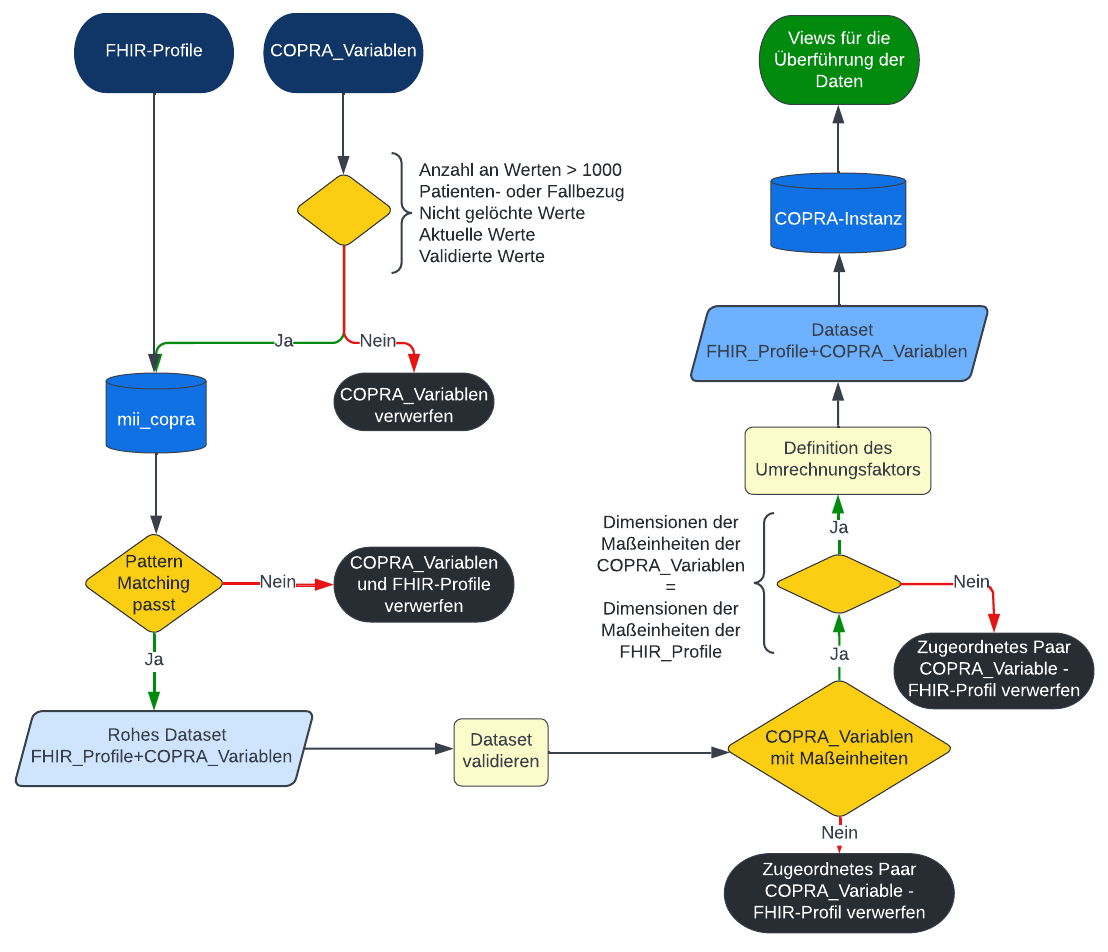
\includegraphics[height=10.5cm]{figures/thesis_flow}
	\caption[Flussdiagramm des Ablaufes des Projekts]{Flussdiagramm des Ablaufes des Projekts.}
	\label{fig:flowdiagram}
\end{figure}	
	\section[Data Mapping der Biosignaldaten aus \acs{copra} mit den \acs{fhir}-Profilen]{Data Mapping der Biosignaldaten aus \\ \acs{copra} mit den \acs{fhir}-Profilen} \label{sec:datamappingicucopra}

Nach der Analyse der \ac{fhir}-Profile des Erweiterungsmoduls \glqq Intensivmedizin\grqq{} und des \ac{copra}-Datenmodells wurden die Daten definiert und ein Pattern Matching-Prozess für die Zuordnung der Biosignaldaten aus \ac{copra} mit den \ac{fhir}-Profilen. Während dieses Verfahrens entstand ein Datensatz. Dieser wurde validiert und für die Zuweisung der Quell- und Zielfelder, und die Programmierung der Transformationsregeln benutzt.

\subsection{Datendefinition} \label{subsec:datadef}

Nach der Analyse des Datenmodells (\ref{fig:copraschema}) wurde die Tabelle mit den Attributen der \ac{fhir}-Profile (\ref{sec:fhirprofs}) zusammen mit den Tabellen von \ac{copra} (\ref{sec:configvarcopra}) untersucht, um zu erkennen, welche \ac{copra}-Tabellen und Spalten mit den Elementen der \ac{fhir}-Profile zu vernetzen sind.

Die Tabelle der \ac{fhir}-Profile (\ref{tab:miiicu}) beinhaltet die Information der Elemente der Profile des Moduls \glqq\ac{icu}\grqq{} des Kerndatensatzes der \ac{mii} und somit die Datenstruktur und Parameter des Zielsystems.

Das Quellsystem dieser Arbeit sind die Tabellen der \ac{copra}-Instanz des Staging Bereichs des \ac{dw} des \ac{diz} an der Universitätsmedizin Mainz. Die Tabelle der Typen der Konfigurationsvariablen (\ref{tab:co6confvartype}) beinhaltet die Datentypen und Namen der Werttabellen, wo die Werte der Biosignaldaten gespeichert sind. In der Tabelle der Konfigurationsvariablen (\ref{tab:co6confvar}) sind die am Standort angegebenen \ac{copra}-Namen und Beschreibungen der Messungen oder angewandten Techniken zusammen mit deren Maßeinheiten zu finden. Eine andere wichtige Tabelle in \ac{copra} ist die mit den Basisdaten der Patienten und Patientinnen (\ref{tab:patient}), wie die Patientennummer. Die Werte und Zeiten der Messungen und Beobachtungen für die Überführung der Daten in die \ac{fhir}-Profile befinden sich in den Werttabellen (\ref{tab:valuetab}, \ref{tab:valuepress}).

Für das Weiterlaufen des Projekts wurden nur die Konfigurationsvariablen ausgewählt, die einen Patientenbezug oder Fallbezug besitzen, mit mindestens 1000 validierten, aktuellen und nicht gelöschten Datensätzen im \ac{copra}-System, denn unter dieser Gruppe befinden sich die Konfigurationsvariablen, die den Biosignaldaten entsprechen.

\subsection{Zuweisung der Quell- und Zielfelder} \label{sec:patternmatchingicucopra}

Nach der Definition der Daten wurden die Quell- und Zielfelder zugewiesen. Um dieses Ziel zu erreichen wurde ein Pattern Matching durchgeführt, um ähnliche Muster zwischen den Parametern der \ac{fhir}-Profile und bestimmten Attributen der Konfigurationsvariablen zu erkennen. 

Für das Pattern Matching wurden zuerst die Namen der \ac{fhir}-Profile zusammen mit den Namen und Beschreibungen der Konfigurationsvariablen mit einer unscharfen Suche mit Hilfe von der Bibliothek \glqq thefuzz\grqq{} in Python analysiert. Diese unscharfe Suche liefert einen Datensatz mit Paaren von Profilen und Konfigurationsvariablen. Anschließend wurden \ac{sql}-Abfragen mit \acp{regex} in den \glqq WHERE\grqq{}-Bedingungen für jedes Profil entwickelt, um falsch zugeordnete Konfigurationsvariablen herauszunehmen und nicht erkannte Konfigurationsvariablen wahrzunehmen. Die Entscheidung der Nutzung von \acp{regex} statt des \ac{sql}-Befehls \glqq LIKE\grqq{} basiert auf der Tatsache, dass die \acp{regex} eine breite Palette an Möglichkeiten bietet, um komplexe Muster zu definieren (\ref{sec:regex}).

Dieser Prozess generierte einen Datensatz mit den zugeordneten Paaren: Konfigurationsvariable - \ac{fhir}-Profil. Dieser Datensatz beinhaltet die wichtigsten Attribute beider Systeme und wurde mit Hilfe der Spezialisten der \ac{pdms}-Abteilung validiert.

Mit dem validierten Datensatz wurden die Attribute der \ac{fhir}-Profile mit den Felder der Tabellen von \ac{copra} zugewiesen, und die Transformationsregel wurden definiert und programmiert.

\subsection{Transformationsregeln} \label{sec:transformrules}

Für die Definition und Programmierung der Transformationsregeln wurden an erster Stelle die Maßeinheiten beider Systeme in dem erzeugten Datensatz nach der Validierung verglichen, um Unregelmäßigkeiten bei diesem Attribut zu detektieren und bestimmte Umwandlungen für die Harmonisierung der Maßeinheiten vorzunehmen. Die Umrechnungen wurden in dem generierten Datensatz des Pattern Matchings eingefügt.

Der resultierende Datensatz wurde in die \ac{copra}-Instanz des Staging Bereichs des \ac{dw} importiert. Mit diesem Datensatz in der \ac{copra}-Instanz, zusammen mit den definierten Spalten mit den Parametern der Biosignaldaten in den Werttabellen, den Spalten mit den Attributen der behandelnden Personen, und Metadaten der Werttabellen, wurden weitere Transformationsregeln für die Überführung der Biosignaldaten aus \ac{copra} in \ac{fhir} programmiert.
	\section{Analyse für die Harmonisierung der Maßeinheiten} \label{sec:units}

Bei der Programmierung der Transformationsregeln ist ein wichtiger Aspekt zu berücksichtigen: die Maßeinheiten der Konfigurationsvariablen und der \ac{fhir}-Profile. Diese Einheiten müssen harmonisiert werden. Um dieses Ziel zu erreichen, wurden die Schreibweise und die Dimensionen der physikalischen Größen der Maßeinheiten analysiert. Konfigurationsvariablen bei denen die Dimensionen der Einheiten nicht mit den von den \ac{fhir}-Profilen übereinstimmen oder die Maßeinheiten im \ac{copra}-System nicht dokumentiert sind, wurden nicht berücksichtigt. Werte in den Werttabellen mit Maßeinheiten derselben Dimensionen, wie bei den \ac{fhir}-Profilen, aber mit anderen Untereinheiten, wurden umgerechnet.

Die Maßeinheiten der \ac{fhir}-Profile wurden bei dem Import in der \ac{db} gleichzeitig analysiert, und die Anmerkungen, wie unterschiedliche Schreibweise derselben Maßeinheit oder Untereinheiten zwischen Profilen, wurden als Issue auf der Webseite von SIMPLIFIER des Moduls \glqq\ac{icu}\grqq{} gemeldet.

Die Konfigurationsvariablen ohne Maßeinheiten wurden den Spezialisten der \ac{pdms}-Abteilung gesendet, denn manche Konfigurationsvariablen beinhalten die Maßeinheiten am Frontend von \ac{copra} und nicht in der \ac{db} des Systems.

Für den Vergleich zwischen den Maßeinheiten der Konfigurationsvariablen von \ac{copra} und der \ac{fhir}-Profile in der \ac{db}, wurde eine \ac{sql}-Abfrage mit integrierten \acp{regex} programmiert. Dieser Schritt ist nicht nur für den Vergleich der Maßeinheiten zwischen beiden Systemen notwendig, sondern auch für die Erkennung von Unregelmäßigkeiten im \ac{copra}-System.

Am Ende dieser Analyse wurde der Datensatz des Pattern Matchings gefiltert, und die zugeordneten Paare von Konfigurationsvariablen und \ac{fhir}-Profile mit Problemen bezüglich der Maßeinheiten wurden herausgenommen. Dieser neue Datensatz wurde in einer neuen Tabelle (\ref{sec:unitscopra}) mit einer neuen Spalte für die Umrechnung der Maßeinheiten für die Harmonisierung in \ac{copra} kopiert. Dieser Datensatz wird wiederum in die \ac{copra}-Instanz des Staging Bereichs des \ac{dw} importiert, um weitere Schritte des Data Mappings durchzuführen.
	\section[Vorbereitung der Überführung der Daten aus \acs{copra} in \acs{fhir}]{ Vorbereitung der Überführung der Daten aus \acs{copra} in \acs{fhir}} \label{sec:docutransfer}

Der erzeugte Datensatz nach der Analyse der Maßeinheiten wurde in die \ac{copra}-Instanz des Staging Bereichs des \ac{dw} importiert, denn der Rest der benötigten Daten für die Erzeugung der \ac{fhir}-Ressourcen des Erweiterungsmoduls \glqq Intensivmedizin\grqq{} befinden sich in verschiedenen Tabellen dieser Instanz. 

Dadurch, dass die notwendigen Daten in \ac{copra} in mehreren Tabellen liegen (\ref{fig:copraschema}), sollten sie hierzu zusammengeführt werden. Die genauen Daten von \ac{copra} und den \ac{fhir}-Profilen des Datensatzes der Zuordnung für die Zusammenführung wurden dann spezifiziert.
Am Ende der Spezifikation wurden \ac{sql}-Views mit den zusammengeführten Parametern und den Transformationsregeln in der \ac{copra}-Instanz programmiert. Diese Views können in weiteren Prozessen bei der Überführung der Biosignaldaten aus \ac{copra} in \ac{fhir} benutzt werden.
	\chapter{Realisierung} \label{ch:results}

Dieses Kapitel befasst sich mit der Realisierung dieses Projekts und die Ereignisse, die währenddessen entstanden sind.

Vor der Realisierung des Projekts ist es wichtig zu wissen, wie die Daten in dem Staging Bereich des \ac{dw} des \ac{diz} an der Universitätsmedizin Mainz gespeichert werden, und wie diese Daten danach im \ac{diz} bearbeitet werden (\ref{fig:dizummz}).

\begin{figure}[ht]
	\centering
	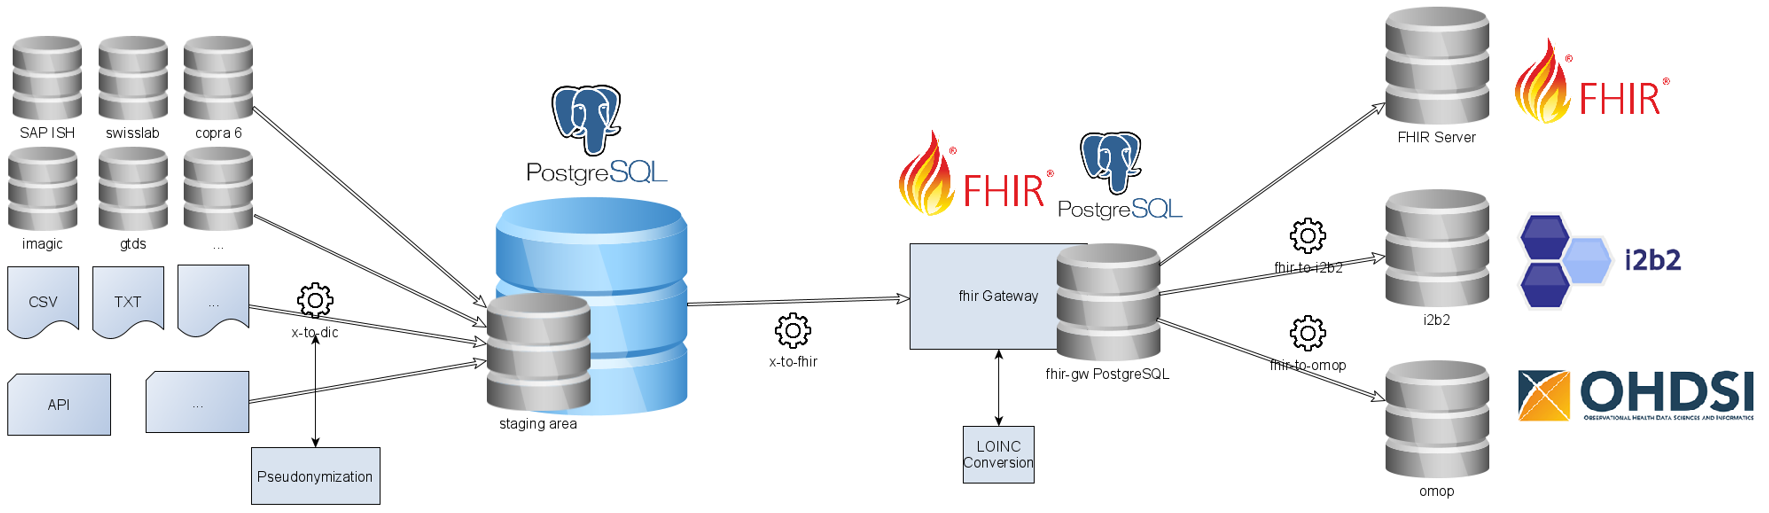
\includegraphics[height=4cm]{figures/diz_ummz}
	\caption[\acs{diz}-Struktur an der Universitätsmedizin Mainz] {\acs{diz}-Struktur an der Universitätsmedizin Mainz. Die Daten aus den verschiedenen Quellen in der Klinik werden pseudonymisiert in dem Staging Bereich des \ac{dw} zur Bearbeitung gespeichert. Diese bearbeiteten Daten werden in \ac{fhir} überführt oder zu anderen \acp{db} transportiert. Am Ende wird die Information mit Hilfe von Werkzeugen, wie i2b2 visualisiert.}
	\label{fig:dizummz}
\end{figure}

 Für die Durchführung dieser Masterarbeit wurde mit der Information der \ac{copra}-Instanz des Staging Bereichs des \ac{dw} gearbeitet (\ref{fig:components}).

 Zu Beginn wurde die \ac{db} \texttt{mii\_copra} entwickelt. In den Tabellen dieser \ac{db} wurden die Parameter der \ac{fhir}-Profile des Erweiterungsmodul \glqq Intensivmedizin\grqq{} zusammen mit den relevanten Konfigurationsvariablen von \ac{copra} importiert. In der \ac{db} \texttt{mii\_copra} wurden auch die Zwischenschritten des Data Mappings realisiert. Als Ergebnis dieses Prozesses entstand der Datensatz mit zugeordneten Konfigurationsvariablen mit \ac{fhir}-Profilen. Die Maßeinheiten im Datensatz wurden harmonisiert. Dieser Datensatz wurde danach in der \ac{copra}-Instanz des Staging Bereichs des \ac{dw} importiert. Mit diesem Datensatz als Basis wurden \ac{sql}-Views für die Zusammenführung der Daten beider Systeme programmiert.

Ein Diagramm mit den Komponenten und dem Fluss der Daten in diesem Projekt ist in der \ref{fig:components} dargestellt.

\begin{figure}[ht]
	\centering
	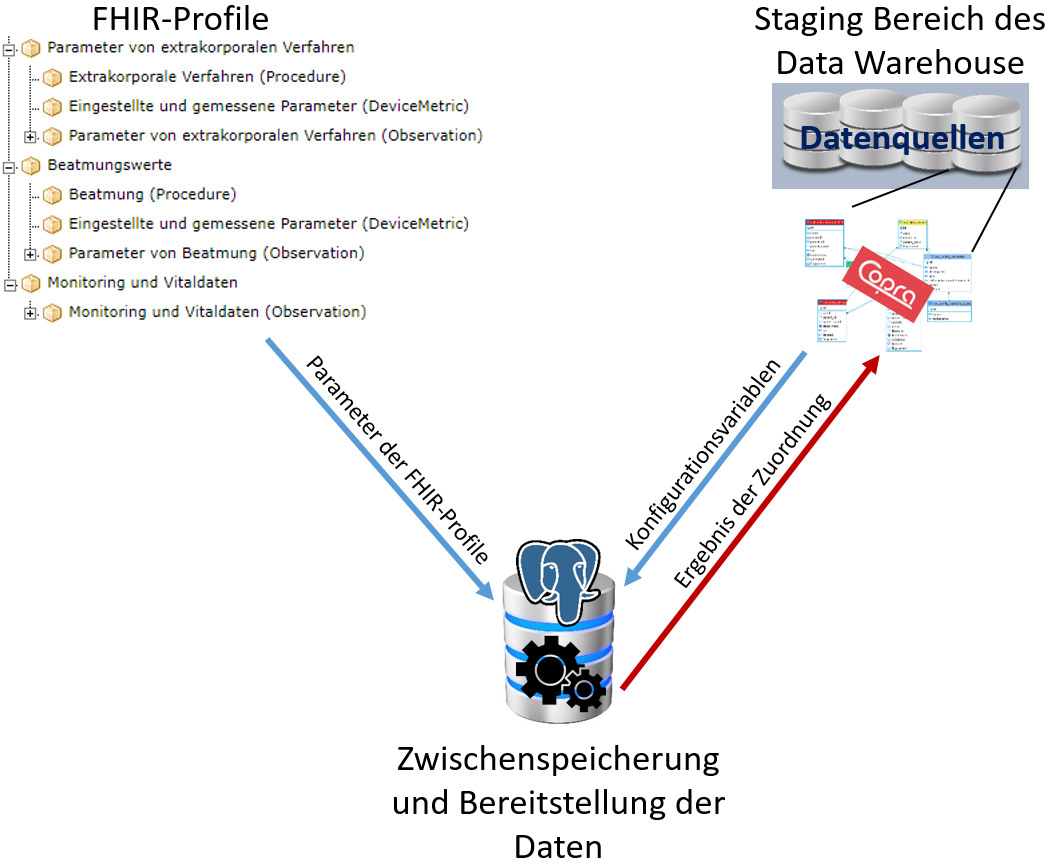
\includegraphics[height=9.5cm]{figures/master_diagram}
	\caption[Komponenten und Fluss der Daten] {Komponenten und Fluss der Daten in diesem Projekt.}
	\label{fig:components}
\end{figure}
	\section{PostgreSQL-\acs{db}} \label{sec:database}

Für die Entwicklung dieses Projekts wurde die \ac{db} \texttt{mii\_copra} in PostgreSQL erstellt, um Attribute der \ac{fhir}-Profile und Parameter der im \ac{copra} gespeicherten Konfigurationsvariablen zu speichern. In dieser \ac{db} fanden auch die Bearbeitung und Analyse der Daten statt.

Die \ac{db} \texttt{mii\_copra} wurde in einer Testumgebung mit PostgreSQL 14.2 unter Linux Ubuntu 22.04.1 \ac{lts} implementiert. Für die Entwicklung der \ac{db} und die weiteren \ac{sql}-Prozesse wurde die Community Version des freien Open Source Werkzeugs \href{https://dbeaver.io/}{DBeaver} benutzt.

In der \ac{db} \texttt{mii\_copra} wurde eine Tabelle angelegt für die Speicherung bestimmter herausgenommener Parameter der \ac{fhir}-Profile der \ac{mii} - Modul \glqq\ac{icu}\grqq{}. Zwei weitere Tabellen sollen die relevanten Attribute der Metadaten von \ac{copra} speichern. Diese Tabellen mit Metadaten 
sammeln die Informationen der Konfigurationsvariablen und Konfigurationsvariablen-Typen und beinhalten unter anderem die Namen und Datentypen der an der Intensivstation und Notaufnahme der Universitätsmedizin Mainz gemessenen Biosignaldaten. In der \ac{db} wurden auch die \ac{sql}-Abfragen für die Zusammenführung der \ac{fhir}-Profile mit den Biosignaldaten geschrieben. Schließlich wurden weitere Tabellen angelegt, um die resultierenden Zwischenergebnisse und Datensätze zu speichern, analysieren und visualisieren (\ref{tab:miiicu}, \ref{tab:mapping}).
	\section{Parameter der \acs{fhir}-Profile des Moduls \glqq\acs{icu}\grqq{}} \label{sec:fhirprofs}

Die Information der \ac{fhir}-Profile des Moduls \glqq\ac{icu}\grqq{} des Kerndatensatzes der \ac{mii} wurde aus der Webseite \href{https://www.medizininformatik-initiative.de/Kerndatensatz/Modul_Intensivmedizin/IGMIIKDSModulICU.html}{Medizininformatik Initiative - Modul ICU - ImplementationGuide} herausgenommen. Obwohl dieses Modul zum Abstimmverfahren von 25.02.2022 bis 08.04.2022 freigeben wurde, befindet es sich noch während der Entwicklung dieses Projekts in der ersten stabilen Ballot-Version. Das bedeutet für diese Arbeit, dass Unregelmäßigkeiten in den Profilen detektiert werden können, und als Issue gemeldet werden.

Die Parameter je Profil an der Webseite, nämlich Name, Typ, Attribute der Maßeinheit, Daten der Codesysteme und vorhandene Metrik des Geräts wurden in die Tabelle \texttt{mii\_icu} der \ac{db} \texttt{mii\_copra} eingefügt.

Die meisten \ac{fhir}-Profile unter der Kategorie \glqq Observation\grqq{} besitzen eine ähnliche Struktur, sodass der Import in die Tabelle \texttt{mii\_icu} erleichtert wird. Die Ausnahmen bilden die Profile der Gruppe \glqq Blutdruck Generisch\grqq{} für die Speicherung der Blutdruckmessungen, z. B. \glqq Linksatrialer Druck\grqq{}. Diese Profile sind eine Zusammensetzung von drei separat kodierten \glqq Observations\grqq{}, die dieselben Attribute teilen, nämlich die Spezifikationen für den systolischen, mittleren und diastolischen Blutdruck. In solchen Fällen wurden auch die semantischen Annotationen der systolischen, mittleren und diastolischen Attribute in der Tabelle \texttt{mii\_icu} registriert.

Die Struktur der Tabelle \texttt{mii\_icu} zur Speicherung der Elemente der \ac{fhir}-Profile ist in der \ref{tab:miiicu} dargestellt.

\begin{longtable}{|p{3.5cm}|l|p{6.7cm}|}
	\caption[Struktur der Tabelle mii\_icu]{Struktur der Tabelle \texttt{mii\_icu}. In dem Feld Spalte befinden sich die gegebenen Namen der \ac{fhir}-Elemente der Profile. Der Datentyp ist der Typ mit dem die Daten in der Tabelle \texttt{mii\_icu} gespeichert werden. Die Spalte Information speichert die Beschreibung des Elements.} \label{tab:miiicu}
	\endfirsthead
		\hline
		\rowcolor{lightgray} Spalte & Datentyp & Information \\ \hline
		profile\_id & int & Generierter nummerischer Identifikator des zugeordneten \ac{fhir}-Profils \\ \hline
		profile\_name & varchar & Name des \ac{fhir}-Profils, z. B. Atemzugvolumen-Waehrend-Beatmung \\ \hline
		category\_coding \_system & text & \acsu{url} der Kategorie \glqq Observation\grqq{}. Dies kann ein \ac{snomedct}-\ac{url} sein \\ \hline
		category\_coding \_code & varchar & \glqq vital-signs\grqq{} oder \ac{snomedct}-ID \\ \hline
		code\_coding \_system\_snomed & text & http://snomed.info/sct \\ \hline 
		code\_coding \_code\_snomed & varchar & \ac{snomedct} des \ac{fhir}-Profils, z. B. 250874002 \\ \hline
		code\_coding \_system\_loinc & text & http://loinc.org \\ \hline
		code\_coding \_code\_loinc & varchar & \ac{loinc}-Code des \ac{fhir}-Profils, z. B. 76222-9 \\ \hline
		code\_coding \_system\_ieee & text & urn:iso:std:iso:11073:10101 \\ \hline
		code\_coding \_code\_ieee & varchar & \ac{iso}/\ac{ieee} 11073-10101\texttrademark{}-Schlüssel des \ac{fhir}-Profils, z. B. 151980 \\ \hline
		valuequantity \_system & text & http://unitsofmeasure.org \\ \hline
		valuequantity\_code & varchar & Maßeinheiten im \ac{fhir}-Profil, z. B. mL \\ \hline
		device\_reference & text & Zuweisung zur Art der Prozedur (gemessen, eingestellt oder erhoben). Diese Prozedur befindet sich in den Profilen der Typ \glqq DeviceMetric\grqq{} \\ \hline
		code\_systolic \_coding\_system \_snomed & text & http://snomed.info/sct \\ \hline
		code\_systolic \_coding\_code \_snomed & varchar & \ac{snomedct}-ID der systolischen Blutdruckmessung, z. B. 271649006 \\ \hline
		code\_systolic \_coding\_system \_loinc & text & http://loinc.org \\ \hline
		code\_systolic \_coding\_code \_loinc & varchar & \ac{loinc}-Code der systolischen Blutdruckmessung, z. B. 8406-1 \\ \hline
		code\_systolic \_coding\_system \_ieee & text & urn:iso:std:iso:11073:10101 \\ \hline
		code\_systolic \_coding\_code \_ieee & varchar & \ac{iso}/\ac{ieee} 11073-10101\texttrademark{}-Schlüssel der systolischen Blutdruckmessung \\ \hline
		code\_mean \_coding\_system \_snomed & text & http://snomed.info/sct \\ \hline
		code\_mean \_coding\_code \_snomed & varchar & \ac{snomedct}-ID der mittleren Blutdruckmessung, z. B. 6797001 \\ \hline
		code\_mean \_coding\_system \_loinc & text & http://loinc.org \\ \hline
		code\_mean \_coding\_code \_loinc & varchar & \ac{loinc}-Code der mittleren Blutdruckmessung, z. B. 8478-0 \\ \hline
		code\_mean \_coding\_system \_ieee & text & urn:iso:std:iso:11073:10101 \\ \hline
		code\_mean \_coding\_code \_ieee & varchar & \ac{iso}/\ac{ieee} 11073-10101\texttrademark{}-Schlüssel der mittleren Blutdruckmessung, z. B. 150019 \\ \hline
		code\_diastolic \_coding\_system \_snomed & text & http://snomed.info/sct \\ \hline
		code\_diastolic \_coding\_code \_snomed & varchar & \ac{snomedct}-ID der diastolischen Blutdruckmessung, z. B. 271650006 \\ \hline
		code\_diastolic \_coding\_system \_loinc & text & http://loinc.org \\ \hline
		code\_diastolic \_coding\_code \_loinc & varchar & \ac{loinc}-Code der diastolischen Blutdruckmessung, z. B. 8462-4 \\ \hline
		code\_diastolic \_coding\_system \_ieee & text & urn:iso:std:iso:11073:10101 \\ \hline
		code\_diastolic \_coding\_code \_ieee & varchar & \ac{iso}/\ac{ieee} 11073-10101\texttrademark{}-Schlüssel der diastolischen Blutdruckmessung, z. B. 150018 \\ \hline
		meta\_profile & text &  \ac{url} um das Profil zu identifizieren \\ \hline
\end{longtable}

	\section{Analyse der \acs{fhir}-Profile des \acs{mii} - Moduls \acs{icu}} \label{sec:fhiricuresult}

Bevor die Parameter der \ac{fhir}-Profile in die \ac{db} importiert wurden, erfolgte eine Analyse der bis dato 80 \ac{fhir}-Profile. 

In dieser Analyse wurde beobachtet, dass zwei Profile dieselben Namen besitzen, aber unterschiedliche Information beinhalten. Diese sind unter dem Profil-Namen \glqq Linksventrikulärer Schlagvolumenindex\grqq{} zu finden. In einem der Profile wird tatsächlich die Information des linksventrikulären Schlagvolumenindex spezifiziert. Das andere Profil hingegen sollte das linksventrikuläre Schlagvolumen definieren. Dieses Ereignis wurde durch das Attribut \glqq code\grqq{} beider Profile erkannt. Dieses Attribut spezifiziert die Codesysteme des Profils. An dieser Stelle wurde beobachtet, dass das Profil für den linksventrikulären Schlagvolumenindex den \ac{loinc}-Code \href{https://loinc.org/76297-1/}{76297-1} \glqq Left ventricular Stroke volume index\grqq{} besitzt. Das Profil für das linksventrikuläre Schlagvolumen beinhaltet wiederum den \ac{loinc}-Code \href{https://loinc.org/20562-5/}{20562-5} \glqq Left ventricular Stroke volume\grqq{}. Noch dazu sind die spezifizierten \ac{snomedct}-IDs und \ac{ieee}-Schlüssel beider Profile im Attribut \glqq code\grqq{} auch unterschiedlich. Diese Problematik wurde in der SIMPLIFIER-Webseite des Moduls vorher korrigiert. Aus diesem Grund wurde diese Anmerkung als Issue nicht gemeldet.

Nach der durchgeführten Analyse der 80 \acs{fhir}-Profile, wurden die \ac{fhir}-Elemente der Profile in die Tabelle \texttt{mii\_icu} der \ac{db} \texttt{mii\_copra} geschrieben. Mit diesen Daten in der \ac{db} wurde die Einteilung der Profile analysiert.

Die \ref{tab:proficu} zeigt die Anzahl an Profilen je Kategorie im Modul \glqq\ac{icu}\grqq{}. Die meist repräsentierten \ac{fhir}-Profile, nämlich 76, gehören zu der Kategorie \glqq Observation\grqq{}.

\begin{table}[ht]
	\centering 
	\caption[\acs{fhir}-Profile im Modul \glqq\acs{icu}\grqq{}]{\acs{fhir}-Profile im Modul \glqq\acs{icu}\grqq{}.}
	\label{tab:proficu}
	\begin{tabular}{|l|l|}
		\hline
		\bfseries Anzahl der Profile & \bfseries Profiltyp \\ \hline
		76 & Observation \\ \hline
		2 & Procedure \\ \hline   
		2 & DeviceMetric \\ \hline
		80 & Gesamt \\ \hline
	\end{tabular}
\end{table}

In den logischen Tabellen der \ac{fhir}-Profile sind die standardisierten Codesysteme der Biosignaldaten im Attribut \glqq code\grqq{} registriert. Dieses Attribut ist charakteristisch für Profile der Typen \glqq Observation\grqq{} und \glqq Procedure\grqq{}. Die Distribution der Codesysteme in der \ac{fhir}-Profile ist in der \ref{tab:profilcodes} dargestellt. Das meist repräsentierte Codesystem ist \ac{loinc} mit 62 Profilen. Aus diesem Grund wurde dieses Codesystem als zusätzlicher Parameter für das Pattern Matching angewendet. Von den 78 \ac{fhir}-Profilen unter den Kategorien \glqq Observation\grqq{} und \glqq Procedure\grqq{} besitzen fünf kein Codesystem.

%\clearpage

\begin{table}[ht]
	\centering 
	\caption[Codesysteme der \acs{fhir}-Profile im Modul \glqq\acs{icu}\grqq{}]{Distribution der Codesysteme der \acs{fhir}-Profile im Modul \glqq\acs{icu}\grqq{}.}
	\label{tab:profilcodes}
	\begin{tabular}{|l|l|}
		\hline
		\bfseries Anzahl der Profile & \bfseries Codesystem \\ \hline		
		62 & \ac{loinc} \\ \hline
		54 & \ac{snomedct} \\ \hline   
		36 & \acs{iso}/\acs{ieee} 11073-10101\texttrademark{} \\ \hline
		5 & - \\ \hline
	\end{tabular}
\end{table}

Die Profile der Typen \glqq Observation\grqq{}, die keine Codesysteme beinhalten (\ref{tab:profilnocode}), gehören zu den generischen Profilen. Diese sind nicht für die direkte Umsetzung konzipiert, sondern zur Modellierung der Daten. Die \glqq Procedure\grqq{}-Profile beinhalten keine Codesysteme, weil sich diese Information im Basismodul \glqq Prozedur\grqq{} des Kerndatensatzes der \ac{mii} befindet. Die Profile unter der Kategorie \glqq DeviceMetric\grqq{} besitzen auch keine Codesysteme, denn diese Profile beschreiben die Messung oder Einstellungen des Geräts (\ref{subsec:icumodul}).

\begin{table}[ht]
	\centering  
	\caption[\glqq Observation\grqq{}-Profile ohne Codesystem]{\glqq Observation\grqq{}-Profile ohne Codesystem.}
	\label{tab:profilnocode}
	\begin{tabular}{|p{8.5cm}|l|}
		\hline 
		\bfseries \ac{fhir}-Profile & \bfseries Profiltyp \\ \hline
		Parameter von extrakorporalen Verfahren & Observation \\ \hline
		Monitoring und Vitaldaten & Observation \\ \hline
		Parameter von Beatmung & Observation \\ \hline
	\end{tabular}
\end{table}

Ein weiterer wichtiger Aspekt ist die Analyse der Maßeinheiten der 76 Profile des Typs \glqq Observation\grqq{}. An dieser Stelle wurden 73 Profile mit definierten und drei ohne definierte Maßeinheiten im Modul gefunden. Diese letzten drei Profile sind dieselben \glqq Observation\grqq{}-Profile ohne Codesysteme (\ref{tab:profilnocode}).

Eine andere Beobachtung hinsichtlich der Maßeinheiten mancher Profile ist, dass die Schreibweise einer Maßeinheit oder deren Untereinheiten bei verschiedenen Profilen nicht immer dieselbe war. Diese Unregelmäßigkeit wurde an die SIMPLIFIER-Webseite des Moduls gemeldet (\href{https://simplifier.net/medizininformatikinitiative-modul-intensivmedizin/~issues/2083}{Issue \#2083}), und von den Autoren und Entwicklern des Moduls korrigiert. Nach der Korrektur wurden die Schreibweisen der Maßeinheiten der \ac{fhir}-Profile in der Spalte \texttt{valuequantity\_code} der Tabelle \texttt{mii\_icu} geändert.

Ein Detail bei der Benennung der Profile ist, dass die Namen von 26 Profilen Umlaute beinhalten. Bei sechs Profilnamen hingegen wurden die Umlaute zusammen mit dem Buchstabe Eszett \glqq ß\grqq{} vermieden. Die \ref{tab:umlaut} zeigt einige Beispiele davon. Dieses Phänomen wurde auch als Issue gemeldet (\href{https://simplifier.net/medizininformatikinitiative-modul-intensivmedizin/~issues/2394}{Issue \#2394}), denn dieselben \ac{fhir}-Profile beinhalten in der Webseite \href{https://simplifier.net/guide/MedizininformatikInitiative-ModulICU-ImplementationGuide/IGMIIKDSModulICU?version=current}{\glqq ImplementationGuide\grqq{}} von SIMPLIFIER ebenso Umlaute oder das Eszett in den Namen.

\begin{table}[ht]
	\centering 
	\caption[An- un Abwesenheit von Umlauten in den Profilnamen]{An- un Abwesenheit von Umlauten in den Profilnamen}
	\label{tab:umlaut}
	\begin{tabular}{|l|}
		\hline 
		\bfseries Namen mit Umlaut \\ \hline
		Hämodialyse Blutfluss \\ \hline 
		Zeitverhältnis-Ein-Ausatmung \\ \hline \hline
		\bfseries Namen ohne Umlaut und ohne Eszett\\ \hline
	    Spontanes-Mechanisches-Atemzugvolumen-Waehrend-Beatmung\\ \hline            
		Koerpergroesse \\ \hline                
	\end{tabular}
\end{table}
	\section{Angepasste Tabellen von \acs{copra}} \label{sec:copratables}

Das Datenmodell der \ac{copra}-Instanz des Staging Bereichs des \ac{dw} des \ac{diz} an der Universitätsmedizin Mainz (\ref{fig:copraschema}) zusammen mit dem Inhalt der Tabellen dieser \ac{copra}-Instanz wurden analysiert, denn in \ac{copra} befinden sich die Daten und Metadaten der Bioparameter. Die Tabellen der \ac{copra}-Instanz beinhalten nicht nur die notwendigen Parameter für die Entwicklung dieses Projekts, sondern auch administrative Attribute, die nicht für die Zwecke dieser Arbeit relevant sind. Aus diesem Grund werden nur die relevanten Spalten für das Data Mapping betrachtet. Infolgedessen wurden gleichnamige angepasste Tabellen für die Tabellen der Metadaten (\texttt{co6\_config\_variables} und \texttt{co6\_config\_variable\_types}) in der \ac{db} \texttt{mii\_copra} für die Bearbeitung der Daten codiert.

Die Tabelle \texttt{co6\_config\_variables} beschreibt die Entitäten im \ac{copra}-System und somit beinhaltet diese Tabelle die Namen und Beschreibungen der Biosignalparameter. In dieser Tabelle wurden nur die Konfigurationsvariablen mit den notwendigen Eigenschaften ausgewählt (\ref{sec:configvarcopra}). Die Dokumentierung der relevanten Spalten von \texttt{co6\_config\_variables} ist in der \ref{tab:co6confvar} dargestellt.

\begin{longtable}{{|p{3cm}|l|p{7.3cm}|}} 
	\caption[Relevante Spalten von co6\_config\_variables]{Relevante Spalten von co6\_config\_variables.}\label{tab:co6confvar}
	\endfirsthead
	\hline  
	\bfseries Spalte & \bfseries Datentyp & \bfseries Information \\ \hline
	id & bigint & Hauptschlüssel der Tabelle, z. B. 100 \\ \hline 
	name & varchar & Name der Konfigurationsvariable in der Tabelle, z. B. AF  \\ \hline 
	description & varchar & Beschreibung oder Name der Entitäten, z. B. Atemfrequenz \\ \hline
	unit & varchar & Maßeinheit, z. B. 1/min \\ \hline  
	co6\_config \_variableTypes\_id & varchar & Datentyp der gespeicherten Werte der Konfigurationsvariable, z. B. decimal\_6\_3 \\ \hline
	parent & varchar & Bezug der Konfigurationsvariable, z. B. Patient \\ \hline
	deleted & varchar & \texttt{null} wenn die Konfigurationsvariable noch in Nutzung ist, sonst Datum der Löschung \\ \hline	
\end{longtable}

Die Tabelle \texttt{co6\_config\_variable\_types} enthält die Datentypen der Konfigurationsvariablen und, unter anderem, die Information in welchen Werttabellen die korrespondierenden Werte der Messungen oder Beobachtungen der Biosignale im \ac{copra} sich befinden. Denn die Daten werden in \ac{copra} in separaten Tabellen je nach Datentyp gespeichert. Die wichtigsten Spalten der Tabelle \texttt{co6\_config\_variable\_types} sind in der \ref{tab:co6confvartype} aufgelistet.

\begin{table}[ht]
	\caption[Relevante Spalten von co6\_config\_variable\_types]{Relevante Spalten von co6\_config\_variable\_types.}
	\label{tab:co6confvartype}
	\begin{tabular}{{|p{3.5cm}|l|p{6.7cm}|}}
		\hline
		\bfseries Spalte & \bfseries Datentyp & \bfseries Information \\ \hline
		id & bigint & Hauptschlüssel der Tabelle, z. B. 2 \\ \hline 
		name & varchar & Name des Datentyps, z. B. String  \\ \hline 
		tableName & varchar & Name der Tabelle, in der die Information im \ac{copra} gespeichert wird, z. B. co6\_data\_string \\ \hline 
	\end{tabular}
\end{table}
\newpage
Eine weitere wichtige Tabelle für die spätere Überführung der Daten ist \texttt{co6\_medic\_data\_patient} (\ref{tab:patient}). Diese beinhaltet die Basisinformation der behandelnden Personen. Diese Tabelle beinhaltet zusammen mit der Patientennummer einen Hauptschlüssel für die Verlinkung der Werte der Biosignaldaten in den Werttabellen mit der korrespondierenden Person. Aus diesem Grund befindet sich dieser Schlüssel als Fremdschlüssel auch in den Werttabellen.
%\clearpage
\begin{longtable}{{|p{3.5cm}|l|p{6.7cm}|}}
	\caption[Relevante Spalten der Tabelle co6\_medic\_data\_patient]{Relevante Spalten von co6\_medic\_data\_patient.}
	\label{tab:patient}
	\endfirsthead
	\hline
	\bfseries Spalte & \bfseries Datentyp & \bfseries Information \\ \hline
	id & bigint & Hauptschlüssel der Tabelle, z. B. 25 \\ \hline
	patid & varchar & Patientennummer \\ \hline
	deleted & boolean & \texttt{false}, wenn die Person noch im System ist, sonst \texttt{true} \\ \hline
\end{longtable}

\subsection{Werttabellen} \label{subsec:valuetables}

Die Werttabellen (\ref{tab:valuetable}) beinhalten die gespeicherten Werte der Konfigurationsvariablen. Diese Tabellen besitzen den Hauptschlüssel der Tabelle \texttt{co6\_config\_variables} als Fremdschlüssel, um die Werte der Biosignaldaten den korrespondierenden Konfigurationsvariablen zuzuordnen. Von diesen Tabellen, genau wie bei den anderen Tabellen, wurden nur die relevanten Spalten für die Überführung der Information von \ac{copra} in \ac{fhir} berücksichtigt.

\begin{table}[ht]
	\centering  
	\caption[Werttabellen in der \acs{copra}-Instanz]{Werttabellen in der \ac{copra}-Instanz des \ac{dw}. Alle Tabellen beinhalten die Hauptschlüssel der Tabellen \texttt{co6\_medic\_data\_patient} und \texttt{co6\_config\_variables} als Fremdschlüssel. Die Tabellen \texttt{co6\_data\_decimal\_6\_3} und \texttt{co6\_data\_string} besitzen eine Spalte \texttt{val} für die Speicherung der Werte oder Parameter der angewandten Techniken. Die Tabelle \texttt{co6\_medic\_pressure} wiederum beinhaltet drei Spalten für die Speicherung der systolischen, mittleren, und diastolischen Werte der Blutdruckmessungen.}
	\label{tab:valuetable}
	\begin{tabular}{|l|l|}
		\hline
		\bfseries Werttabelle & \bfseries Datentypen \\ \hline
		co6\_data\_decimal\_6\_3 & numerische Werte \\ \hline
		co6\_data\_string & Zeichenketten \\ \hline
		co6\_medic\_pressure & Blutdruckmessungen \\ \hline
	\end{tabular}
\end{table}

Die Werttabellen \texttt{co6\_data\_decimal\_6\_3} und \texttt{co6\_data\_string} besitzen eine ähnliche Struktur. Der Unterschied zwischen beiden Tabellen liegt darin, dass die Spalte \texttt{val} in der Tabelle \texttt{co6\_data\_decimal\_6\_3} die numerischen Werte der Messungen registriert und diese Spalte in der Tabelle \texttt{co6\_data\_string} die Zeichenketten-Elemente erfasst. Wie bei anderen Tabellen im \ac{copra}-System wurden nur die wichtigen Attribute für diese Arbeit ausgewählt. Die Struktur der Tabellen \texttt{co6\_data\_decimal\_6\_3} und \texttt{co6\_data \_string} ist in der \ref{tab:valuetab} dargestellt.

\begin{longtable}{|l|l|p{7cm}|}
	\caption[Relevante Spalten von co6\_data\_decimal\_6\_3 und \\ co6\_data\_string]{Relevante Spalten von co6\_data\_decimal\_6\_3 und co6\_data\_string.}
	\label{tab:valuetab}
	\endfirsthead
		\hline
		\bfseries Spalte & \bfseries Datentyp & \bfseries Information \\ \hline
		id & bigint & Hauptschlüssel der Tabelle, z. B. 2595 \\ \hline
		varid & int & Fremdschlüssel, der zur Spalte id in der Tabelle co6\_config\_variables zeigt, z. B. 102 \\ \hline
		deleted & boolean & \texttt{false}, wenn der Wert noch im System ist, sonst \texttt{true} \\ \hline
		parent\_id & bigint & Fremdschlüssel, der zur Spalte id in der Tabelle co6\_data\_patient zeigt, wenn das Wert von parent\_id gleich 1 ist \\ \hline
		parent\_varid & int & Fremdschlüssel, der zur Spalte id in der Tabelle co6\_config\_variables zeigt. Diese Spalte is der Bezug der Biosignaldaten, z. B. 1 für Patientenbezug \\ \hline
		datetimeto & timestamp & Datum und Uhrzeit der Messung in \acs{iso} 8601 Format (JJJJ-MM-DD HH:mm:ss)\\ \hline
		validated & boolean & \texttt{true} wenn den Eintrag validiert wurde, sonst \texttt{false}. \\ \hline
		flagcurrent & boolean & \texttt{true} wenn den Eintrag noch aktuell ist, sonst \texttt{false}. \\ \hline
		val & numeric/varchar & Wert der Biosignaldaten. Der Wert ist eine Zahl in der Tabelle co6\_data\_decimal\_6\_3, z. B. 38, und eine Zeichenkette in der Tabelle co6\_data\_string, z. B. blass \\ \hline
\end{longtable}

Die Werttabelle \texttt{co6\_medic\_pressure} (\ref{tab:valuepress}) beinhaltet die systolischen, mittleren und diastolischen Blutdruckwerte.

\begin{longtable}{|l|l|p{8cm}|}
	\caption[Relevante Spalten von co6\_medic\_pressure]{Relevante Spalten von co6\_medic\_pressure.}
	\label{tab:valuepress}
	\endfirsthead
		\hline
		\bfseries Spalte & \bfseries Datentyp & \bfseries Information \\ \hline
		id & bigint & Hauptschlüssel der Tabelle, z. B. 2595 \\ \hline
		varid & int & Fremdschlüssel, der zur Spalte id in der Tabelle co6\_config\_variables zeigt, z. B. 102 \\ \hline
		deleted & boolean & \texttt{false}, wenn der Wert noch im System ist, sonst \texttt{true} \\ \hline
		parent\_id & bigint & Fremdschlüssel, der zur Spalte id in der Tabelle co6\_data\_patient zeigt, wenn das Wert von parent\_id gleich 1 ist \\ \hline
		parent\_varid & int & Fremdschlüssel, der zur Spalte id in der Tabelle co6\_config\_variables zeigt. Diese Spalte is der Bezug der Biosignaldaten, z. B. 1 für Patientenbezug \\ \hline
		datetimeto & timestamp & Datum und Uhrzeit der Messung in \acs{iso} 8601 Format (JJJJ-MM-DD HH:mm:ss)\\ \hline
		validated & boolean & \texttt{true} wenn den Eintrag validiert wurde, sonst \texttt{false}. \\ \hline
		flagcurrent & boolean & \texttt{true} wenn den Eintrag aktuell ist, sonst \texttt{false}. \\ \hline
		systolic & numeric & Systolischer Blutdruckwert, z. B. 120 \\ \hline
		mean & numeric & Mittel Blutdruckwert, z. B. 100 \\ \hline
		diastolic & numeric & Diastolischer Blutdruckwert, z. B. 80 \\ \hline
\end{longtable}

Die Zusammenführung von Parametern der Tabellen \texttt{co6\_config\_varia bles}, \texttt{co6\_medic\_data\_patient} und der Werttabellen, zusammen mit manche Komponenten der Tabelle \texttt{mii\_icu} bilden am Ende die \ac{fhir}-Ressourcen des Erweiterungsmoduls \glqq Intensivmedizin\grqq{} ab.
	
	\section{Auswahl der Konfigurationsvariablen von \acs{copra}} \label{sec:configvarcopra}

Die Tabelle \texttt{co6\_config\_variables} in Zusammenhang mit den Werttabellen wurde untersucht, um die relevanten Konfigurationsvariablen für die Durchführung der Arbeit zu erkennen. Die Tabelle \texttt{co6\_config\_variables} beinhaltet 7409 Konfigurationsvariablen.
%\newpage
Die Kriterien für die Wahl der Variablen sind Folgende:

\begin{itemize}
	\item Variablen in Benutzung: Spalte \texttt{deleted} der Tabelle der Konfigurationsvariablen hat den Wert \texttt{null}
	\item Variablen mit validierten Werten in den Werttabellen: Spalte \texttt{validated} hat den Wert \texttt{true}
	\item Variablen mit nicht gelöschten Werten in den Werttabellen: Spalte \texttt{deleted} der Werttabelle hat den Wert \texttt{false}
	\item Variablen mit aktuellen Werten in den Werttabellen: Spalte \texttt{flagCurrent} der Werttabelle hat den Wert \texttt{true}
	\item Variablen mit Patienten- oder Fallbezug: Spalte \texttt{parent} der Tabelle der Konfigurationsvariablen hat die Werte \texttt{1} für Patientenbezug oder \texttt{20} für Fallbezug
	\item Variablen mit 1000 Werten oder mehr in den Werttabellen
\end{itemize}

Um die Konfigurationsvariablen auszuwählen, wurde für jede Werttabelle eine \ac{sql}-Abfrage, wie im Code \ref{list:selectconfigvar}, realisiert.

\begin{lstlisting}[language=SQL, caption={[SQL-Abfrage zur Auswahl der Konfigurationsvariablen] SQL-Abfrage zur Auswahl der Konfigurationsvariablen im COPRA-System. \glqq copra.value\_table cvt\grqq{} stellt die verschiedenen Werttabellen im System dar: co6\_data\_decimal\_6\_3, co6\_data\_string und co6\_medic\_pressure. \glqq quantity\_in\_value\_table\grqq{} ist ein Alias für die Spalte der Menge an Werten in den Werttabellen.}, captionpos=b, label=list:selectconfigvar]
	select 
	count(cvt.id) quantity_in_value_table, -- Menge an Werten je Konfigurationsvariable in der Werttabelle
	ccv.id, -- ID der Konfiguationsvariable
	ccv."name" -- Name der Konfigurationsvariable
	from copra.co6_config_variables ccv  -- Tabelle der Konfigurationsvariablen 
	join copra.value_table cvt -- eine der Werttabellen
	on cvt.varid = ccv.id -- Verlinkung der Werttabele mit der Tabelle co6_config_variables
	where not cdd.deleted -- nicht geloeschte Daten
	and ccv.parent in (1, 20) -- Patienten- oder Fallbezug
	and not ccv.deleted -- Konfigurationsvariable wird benutzt
	and cvt.flagcurrent -- aktuelle Daten
	and cvt.validated -- validierte Daten
	group by ccv.id, ccv."name" 
	having count(cvt.id) >= 1000 -- 1000 Werte oder mehr in den Werttabellen
	order by quantity_in_value_table -- Menge an Werten absteigend sortiert
	;
\end{lstlisting}

Von den 7409 Konfigurationsvariablen in der \ac{copra}-Instanz wurden 701 als relevante Variablen identifiziert. Unter diesen befinden sich die Biosignalparameter für die Zuordnung mit den \ac{fhir}-Profilen.

Die Anzahl der ausgewählten Konfigurationsvariablen in den Werttabellen für das Pattern Matching der Variablen mit den \ac{fhir}-Profilen für die Erkennung der Biosignaldaten in \ac{copra} ist in der \ref{tab:configvarvaluetables} dargestellt.

\begin{table}[ht]
	\centering  
	\caption[Anzahl der repräsentierten Konfigurationsvariablen in je Werttabelle]{Anzahl der repräsentierten Konfigurationsvariablen in je Werttabelle. Die meisten Konfigurationsvariablen sammeln numerische Werte.}
	
	\label{tab:configvarvaluetables}
	\begin{tabular}{|r|l|}
		\hline
		\bfseries Anzahl & \bfseries Werttabelle \\ \hline
		492 & \texttt{co6\_data\_decimal\_6\_3} \\ \hline
		199 & \texttt{co6\_data\_string} \\ \hline
		10 & \texttt{co6\_medic\_pressure} \\ \hline
		701 & Gesamt \\ \hline 
	\end{tabular}
\end{table}

Unter der 701 ausgewählten Konfigurationsvariablen befinden sich die Biosignaldaten für die Datenzuordnung mit den \ac{fhir}-Profilen.
	\section{Analyse der Tabellen für die Datendefinition} \label{sec:analysiscolums}

Mit der Information der relevanten Parameter von \ac{copra} zusammen mit den Parametern der \ac{fhir}-Profile, wurden die geeigneten Spalten der Tabellen von \ac{copra} und der Tabelle \texttt{mii\_icu} in der \ac{db} \texttt{mii\_copra} ausgewählt, die die Parameter für die Überführung der Biosignaldaten in \ac{fhir} beinhalten.

Die Spalten \texttt{profile\_name} und \texttt{loinc} in der Tabelle \texttt{mii\_icu} (\ref{tab:miiicu}), und die Spalten \texttt{name} und \texttt{description} in der Tabelle \texttt{co6\_config \_variables} (\ref{tab:co6confvar}) wurden als geeignete Kandidaten ausgewählt, um die Konfigurationsvariablen aus \ac{copra} mit den \ac{fhir}-Profilen miteinander zu verlinken, denn diese Spalten beinhalten die Hauptinformation für den späteren Zuordnungsprozess.
 
 Einerseits beinhaltet die Spalte \texttt{profile\_name} die Namen der \ac{fhir}-Profile, die wiederum auch die Namen von Verfahren oder Messungen sind, andererseits ist \ac{loinc} das meist verwendete Codesystem in den \ac{fhir}-Profilen (\ref{tab:profilcodes}). Nach der Analyse der gespeicherten \ac{loinc}-Codes wurden auch Abkürzungen gefunden, die für den späteren Pattern Matching-Prozess von Bedeutung sind, denn sie dienen als zusätzliche Namen \glqq Short Name\grqq{} in der Beschreibung der \ac{loinc}-Codes. Manche dieser \glqq Short Names\grqq{} werden auch in der alltäglichen Kommunikation unter dem Gesundheitspersonal benutzt. Diese Besonderheit ist in der \ref{tab:shortname} dargestellt. Solche \glqq Short Names\grqq{} mit einigen Variationen wurden auch in den Namen und Beschreibungen von den Konfigurationsvariablen in \ac{copra} erkannt.

\begin{table}[ht]
	\centering 
	\caption[Beispiel von \acs{loinc}-\glqq Short Name\grqq{}]{Beispiel von \acs{loinc}-\glqq Short Name\grqq{}. Das \ac{fhir}-Profil \glqq Sauerstofffraktion\grqq{} hat den \ac{loinc}-Code, \href{https://loinc.org/71835-3/}{71835-3}. Dieser wiederum besitzt den \glqq Short Name\grqq{} FIO2.}
	\label{tab:shortname}
	\begin{tabular}{|p{4cm}|l|l|}
		\hline
		\bfseries Profile-Name & \bfseries \ac{loinc}-URL & \bfseries Short Name \\ \hline
		Sauerstofffraktion & \url{https://loinc.org/71835-3/} & 
		FIO2 \\ \hline 
	\end{tabular}
\end{table}

In der Tabelle \texttt{co6\_config\_variables} sind die an dem Standort angegebenen \ac{copra}-Namen für Messungen oder Techniken. Diese sind in der Spalte \texttt{name} registriert. Die \ac{copra}-Namen können Fachtermini oder eine Zusammensetzung von Namensabkürzungen des angewandten Verfahrens und Namensabkürzungen des Gerätes sein. Manche der Abkürzungen des Verfahrens sind Varianten des vorher erläuterten \ac{loinc}-\glqq Short Name\grqq{}. Sodass mit Hilfe von den \ac{loinc}-\glqq Short Names\grqq{} auch Konfigurationsvariablen bei dem Pattern Matching Prozess erkannt werden können. Diese Details der \ac{copra}-Namen führten dazu, dass die Spalte \texttt{description} für die Zuordnung der Konfigurationsvariablen mit den \ac{fhir}-Profilen betrachtet werden sollte, denn diese Spalte beinhaltet eine kurze Beschreibung der Verfahren.

Die Maßeinheiten der Konfigurationsvariablen und somit der Biosignaldaten befinden sich in der Spalte \texttt{unit} der Tabelle \texttt{co6\_config\_variables}. Andererseits befinden sich die Maßeinheiten der Profile in der Spalte \texttt{valuequan tity\_code} der Tabelle \texttt{mii\_icu}. Die Maßeinheiten sind entscheidend, da diese in beiden Systemen vergleichbar sein müssen. Das bedeutet, dass die Maßeinheiten beider Systeme dieselben Dimensionen der physikalischen Größen besitzen müssen, sodass eine Umrechnung zwischen den Einheiten beider Systeme möglich ist.

Dadurch dass ein Identifikator der Patienten in den \ac{fhir}-Profilen als Referenz zu der \ac{fhir}-Ressource \glqq Patient\grqq{} in dem Kerndatensatz der \ac{mii} benutzt wird, um die Biosignaldaten zu den korrespondierenden, behandelnden Personen zu verlinken, werden solchen Parameter vom \ac{copra}-System benötigt. Diese Information befindet sich in der Tabelle \texttt{co6\_medic\_patient} in der Spalte \texttt{patid}. Der Inhalt dieser Spalte ist ein Pseudonym der Patientennummer im \ac{kis}. Auch in der Tabelle \texttt{co6\_medic\_patient} (\ref{tab:patient}) soll  die Spalte \texttt{id} berücksichtigt werden, denn diese ist der primäre Schlüssel dieser Tabelle und ist somit Fremdschlüssel in den Werttabellen. Damit werden die Daten der Patienten mit ihren Biosignaldaten im \ac{copra}-System verknüpft. Die Spalte \texttt{deleted} in der Tabelle \texttt{co6\_medic\_patient} wird benötigt, um über die Löschung einer Person aus dem System in Kenntnis gesetzt zu werden.

Die Werte und Zeitangaben der Messungen und Beobachtungen für die Überführung der Daten in die \ac{fhir}-Profile befinden sich in den Werttabellen. Diese Werte sind in der Spalte \texttt{val} der Tabellen \texttt{co6\_data\_decimal\_6\_3} und \texttt{co6\_data\_string} (\ref{tab:valuetab}), und in den Spalten \texttt{systolic}, \texttt{mean} und \texttt{diastolic} der Tabelle \texttt{co6\_medic\_pressure} (\ref{tab:valuepress}) zu finden. Die Zeiten der Messungen sind in der Spalte \texttt{datetimeto} aller Werttabellen zu finden.

 Die Werttabellen beinhalten den Hauptschlüssel der Tabelle \texttt{co6\_medic \_patient} in der Spalte \texttt{parent\_id} als Fremdschlüssel, wenn der Wert diese Spalte gleich 1 ist. Damit wird die Information der Biosignaldaten den Patienten zugewiesen. In der Spalte \texttt{var\_id} ist der Schlüssel der Konfigurationsvariable in der Tabelle \texttt{co6\_config\_variables} für die Zuweisung der Variablen mit den Werten der Biosignale zu finden. Der Hauptschlüssel einer Werttabelle (\texttt{id}) in Kombination mit dem Namen der Werttabelle wird benutzt, um einen Ersatzschlüssel für die Überführung der Daten von \ac{copra} in \ac{fhir}-Ressourcen zu erstellen.

Nach der Datendefinition wird die Zuordnung der Konfigurationsvariablen mit den \ac{fhir}-Profilen durch das Pattern Matching durchgeführt und das Ergebnis in der Tabelle \texttt{mapping\_mii\_co6} (\ref{tab:mapping}) gespeichert.

\begin{longtable}{|p{3.5cm}|l|p{6.5cm}|}
	\caption[Tabelle für die Speicherung der Zuordnung der Konfigurationsvariablen mit den \acs{fhir}-Profilen]{Tabelle für die Speicherung der Zuordnung der Konfigurationsvariablen mit den \acs{fhir}-Profilen nach dem Pattern Matching. Die Spalten mit \texttt{coding\_system} in den Namen speichern die \ac{uri} (Anhang \ref{sec:uri}) der Terminologie-Systeme.}
	\label{tab:mapping}
	\endfirsthead
	\hline			
		\bfseries Spalte & \bfseries Datentyp & \bfseries Information \\ \hline		
		profile\_id & int & Generierter numerischer Identifikator des zugeordneten \ac{fhir}-Profils \\ \hline
		profile\_name & varchar & Name des \ac{fhir}-Profils, z. B. Atemzugvolumen-Waehrend-Beatmung \\ \hline
		category\_coding \_system & text & \acsu{url} der Kategorie. Dies kann ein \ac{snomedct}-\ac{url} bei einigen \glqq Observations\grqq{} sein. \\ \hline
		category\_coding \_code & varchar & \glqq vital-signs\grqq{} oder \ac{snomedct}-ID \\ \hline
		code\_coding \_system\_snomed & text & http://snomed.info/sct \\ \hline 
		code\_coding \_code\_snomed & varchar & \ac{snomedct} des \ac{fhir}-Profils, z. B. 250874002 \\ \hline
		code\_coding \_system\_loinc & text & http://loinc.org \\ \hline
		code\_coding \_code\_loinc & varchar & \ac{loinc}-Code des \ac{fhir}-Profils, z. B. 76222-9 \\ \hline
		code\_coding \_system\_ieee & text & urn:iso:std:iso:11073:10101 \\ \hline
		code\_coding \_code\_ieee & varchar & \ac{iso}/\ac{ieee} 11073-10101\texttrademark{}-Schlüssel des \ac{fhir}-Profils, z. B. 151980 \\ \hline
		valuequantity \_system & text & http://unitsofmeasure.org \\ \hline
		valuequantity\_code & varchar & Maßeinheiten im \ac{fhir}-Profil, z. B. mL \\ \hline
		conf\_var\_unit & varchar & Maßeinheiten der Konfigurationsvariable in \ac{copra}, z. B. ml \\ \hline
		device\_reference & text & Zuweisung zur Art der Prozedur (gemessen, eingestellt oder erhoben). Diese Prozedur befindet sich in den Profilen des Typs \glqq DeviceMetric\grqq{} \\ \hline
		meta\_profile & text &  \ac{url} um das Profil zu identifizieren \\ \hline
		conf\_var\_id & bigint & Primärer Schlüssel der Tabelle \texttt{co6\_config\_variables}, z. B. 104726 \\ \hline
		conf\_var\_parent\_id & bigint & Schlüssel des Bezuges der Variable, z. B. 1 für Patientenbezug \\ \hline
		conf\_var\_parent \_name & varchar & Name des Bezuges, z. B. Patient \\ \hline
		conf\_var\_name & varchar & Name der Konfigurationsvariable, z. B. Beatmung\_MS\_Pallas\_Vt \\ \hline
		conf\_var\_description & varchar & Beschreibung der Konfiguratiovsvariable, z. B. gemessenes Tidalvolumen \\ \hline
		conf\_var\_types\_id & int & Schlüssel des Datentyps in der Tabelle \texttt{co6\_config\_variable\_types}, z. B. 6 für nummerische Werte \\ \hline
		conf\_var\_types\_name & varchar & Name des Datentyps in der Tabelle \texttt{co6\_config\_variable\_types}, z. B. Decimal\_6\_3 \\ \hline
		code\_systolic \_coding\_system \_snomed & text & http://snomed.info/sct \\ \hline
		code\_systolic \_coding\_code \_snomed & varchar & \ac{snomedct}-ID der systolischen Blutdruckmessung, z. B. 271649006 \\ \hline
		code\_systolic \_coding\_system \_loinc & text & http://loinc.org \\ \hline
		code\_systolic \_coding\_code \_loinc & varchar & \ac{loinc}-Code der systolischen Blutdruckmessung, z. B. 8406-1 \\ \hline
		code\_systolic \_coding\_system \_ieee & text & urn:iso:std:iso:11073:10101 \\ \hline
		code\_systolic \_coding\_code \_ieee & varchar & \ac{iso}/\ac{ieee} 11073-10101\texttrademark{}-Schlüssel der systolischen Blutdruckmessung, z. B. 150107 \\ \hline
		code\_mean \_coding\_system \_snomed & text & http://snomed.info/sct \\ \hline
		code\_mean \_coding\_code \_snomed & varchar & \ac{snomedct}-ID der mittleren Blutdruckmessung, z. B. 6797001 \\ \hline
		code\_mean \_coding\_system \_loinc & text & http://loinc.org \\ \hline
		code\_mean \_coding\_code \_loinc & varchar & \ac{loinc}-Code der mittleren Blutdruckmessung, z. B. 8478-0 \\ \hline
		code\_mean \_coding\_system \_ieee & text & urn:iso:std:iso:11073:10101 \\ \hline
		code\_mean \_coding\_code \_ieee & varchar & \ac{iso}/\ac{ieee} 11073-10101\texttrademark{}-Schlüssel der mittleren Blutdruckmessung, z. B. 150019 \\ \hline
		code\_diastolic \_coding\_system \_snomed & text & http://snomed.info/sct \\ \hline
		code\_diastolic \_coding\_code \_snomed & varchar & \ac{snomedct}-ID der diastolischen Blutdruckmessung, z. B. 271650006 \\ \hline
		code\_diastolic \_coding\_system \_loinc & text & http://loinc.org \\ \hline
		code\_diastolic \_coding\_code \_loinc & varchar & \ac{loinc}-Code der diastolischen Blutdruckmessung, z. B. 8462-4 \\ \hline
		code\_diastolic \_coding\_system \_ieee & text & urn:iso:std:iso:11073:10101 \\ \hline
		code\_diastolic \_coding\_code \_ieee & varchar & \ac{iso}/\ac{ieee} 11073-10101\texttrademark{}-Schlüssel der diastolischen Blutdruckmessung, z. B. 150018 \\ \hline
		matching\_valide & bool & Ergebnis der Validierung der Zuordnung, \texttt{true} oder \texttt{false} \\ \hline
\end{longtable}	
	\section{Pattern Matching der \acs{fhir}-Profile mit den Konfigurationsvariablen} \label{sec:pattmach}

Nach der Erkennung der 701 relevanten Konfigurationsvariablen und der Datendefinition, wurde das Pattern Matching durchgeführt, um bestimmte Muster zwischen Parametern der \ac{fhir}-Profile und Attributen der \ac{copra}-Konfigurationsvariablen zu erkennen. 

Der erste Schritt für das Pattern Matching war die Zuordnung der \ac{fhir}-Profile mit den Konfigurationsvariablen durch eine unscharfe Suche. Für diesen Zweck wurden der Parameter \texttt{profile\_name} der Tabelle \texttt{mii\_icu} zusammen mit den Parametern \texttt{name} und \texttt{description} der Tabelle \texttt{co6\_config \_variables} in einem \ac{csv}-Datei extrahiert. 

Mit einem Python-Skript und der extrahierten \ac{csv}-Datei wurde die unscharfe Suche durchgeführt. Dieser Prozess liefert einen Datensatz mit 400 Paaren von zugeordneten Profilen mit Konfigurationsvariablen. 355 Paare davon waren falsche Zuordnungen, wie die Beispiele der \ref{tab:wrongpaar} zeigen.

\begin{lstlisting}[language=python, caption={[Python-Skript für das Pattern Matching] Python-Skript für das Pattern Matching. Die Option \glqq token\_set\_ratio\grqq{} ermöglicht eine flexiblere fuzzy-Suche (\ref{sub:levdist}), denn die Länge der Namen der Profile und die Länge der Namen und Beschreibungen der Konfigurationsvariablen sind deutlich unterschiedlich.} , captionpos=b, label=list:testr]
from thefuzz import process, fuzz  # Bibliotheken laden

with open("profils_names.csv") as fp: # Datei mit den Namen der Profile
prn = fp.readlines() # Name der Profile
prn = [x.strip() for x in prn] 

with open("config_vars_names.csv") as fc: # Datei mit den Konfigurationsvariablen
cvn = fc.readlines() # Konfigurationsvariablen
cvn = [x.strip() for x in cvn]

for profil in prn: # Bei jeden Namen der Profile
  match_ratios = process.extract(profil, cvn, scorer=fuzz.token_set_ratio) # Liste der passenden Konfigurationsvariablen.
  for prn_match_cvn in match_ratios: 
    print(profil, prn_match_cvn) # Liste der Paare "Profile - Konfigurationsvariablen"
   
\end{lstlisting}

\begin{table}[ht]
	\centering 
	\caption[Beispiele von falsch zugeordneten \acs{fhir}-Profilen]{Beispiele von falsch zugeordneten \acs{fhir}-Profilen. Die Namen der Konfigurationsvariablen und deren Beschreibung sind durch \glqq-\grqq{} getrennt.}
	\label{tab:wrongpaar}
	\begin{tabular}{|l|l|}
		\hline
		\bfseries Profile & \bfseries Konfigurationsvariablen \\ \hline
		Arterieller Druck & ICP - Intrakranialer Druck \\ \hline
		Atemfrequenz & HF - Herzfrequenz \\ \hline
        Rechtsatrialer Druck & CPP - Zerebraler Perfusionsdruck \\ \hline
        Venoeser Druck & PAP - Pulmunalarterieller Druck \\ \hline
	\end{tabular}
\end{table}

Nach dem vorherigen Ergebnis der unscharfen Suche wurden die \ac{fhir}-Profile und die Konfigurationsvariablen nochmal analysiert. Dieses Mal mit \ac{sql}-Abfragen mit \acp{regex} in den WHERE-Bedingungen. Für dieses Verfahren wurden Informationen der Spalten \texttt{profile\_name} und \texttt{loinc} der Tabelle \texttt{mii\_icu} benutzt, um Muster in den Spalten \texttt{name} und \texttt{description} der Tabelle \texttt{co6\_config\_variables} zu identifizieren. Die \ref{fig:mapping} zeigt eine Darstellung der angewandten Parameter der Tabellen und deren Zusammenführung in dem Pattern Matching-Prozess.

\clearpage

\begin{figure}[ht]
	\centering
	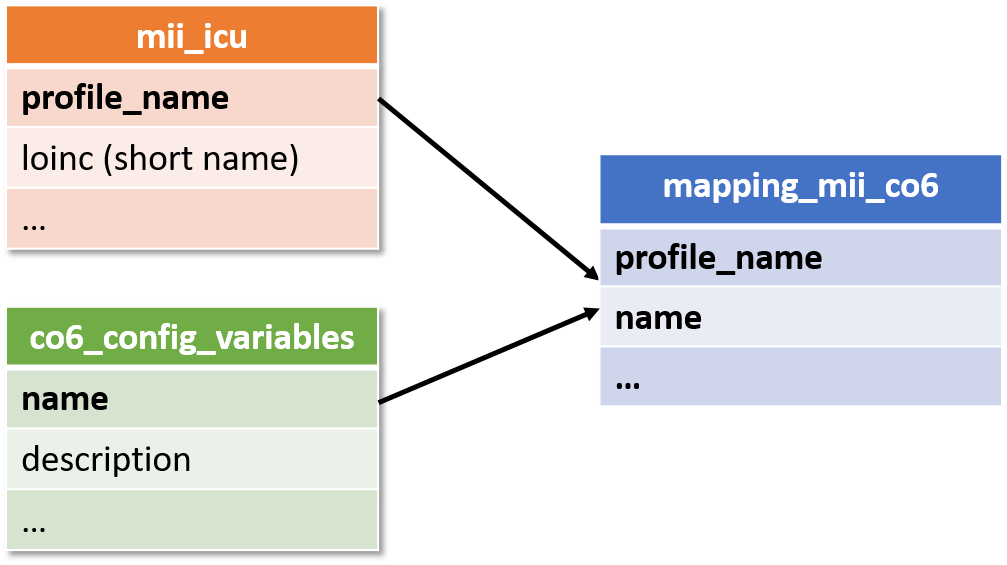
\includegraphics[height=5.5cm]{figures/mapping}
	\caption[Zuordnung der Konfigurationsvariablen mit den \acs{fhir}-Profilen]{Schematische Darstellung der Zuordnung der Spalte \texttt{profile\_name} und die \glqq Short Names\grqq{} der \acs{loinc}-Codes in der Spalte \texttt{loinc} der Tabelle \texttt{mii\_icu} mit den Spalten \texttt{name} und \texttt{description} der Tabelle \texttt{co6\_config\_variables}. Das Ergebnis der Zuordnung wird in der Tabelle \texttt{mapping\_mii\_co6} gespeichert.}
	\label{fig:mapping}
\end{figure}

Wichtig für die Definition der \acs{regex} bei der Anwendung dieses Verfahrens ist die Auswahl von Teilwörtern (\ref{subsec:pattmatch}) oder Kombinationen davon, die die \ac{fhir}-Profile charakterisieren. Denn diese Teilwörter sind in den meisten Fällen Fachtermini oder Teile von Fachbegriffen und können wieder in den Namen oder Beschreibungen der Konfigurationsvariablen gefunden werden.

 Manche Teilwörter in den Profilnamen sind sehr allgemein und befinden sich in mehreren Profilen und auch in zahlreichen Namen und Beschreibungen der Konfigurationsvariablen, z. B. \glqq druck\grqq{}. Das hat zufolge, dass viele Konfigurationsvariablen falsch einem Profil durch die Nutzung von nur einem von diesen Teilwörtern zugeordnet werden könnten. Solche Teilwörter wurden in Kombination mit anderen benutzt, um das Pattern Matching zu verfeinern und die Trefferquote zu erhöhen. Hier ist auch die Menge und Länge der angewandten Teilwörter entscheidend, denn die Anwendung von vielen oder zu langen Teilwörtern liefert auch kein Ergebnis. Aus diesem Grund wurde bei der Schreibung der \ac{sql}-Abfragen je \ac{fhir}-Profil solange die Definition der \ac{regex} getestet, bis die optimale Menge und Länge der Teilwörter in der \ac{regex} gefunden wurde, die die genaue Menge an Konfigurationsvariablen geliefert hatten.

Der Code \ref{list:pattdruck} zeigt beispielhaft die \ac{sql}-Abfrage mit \ac{regex} für die gleichzeitige Erkennung mehrerer allgemeiner Teilwörter des Profils \glqq Mittlerer Beatmungsdruck\grqq{} in der Tabelle der Konfigurationsvariablen, um \ac{fhir}-Profile und Konfigurationsvariablen zu zuordnen.
\clearpage
\begin{lstlisting}[language=SQL, caption={[SQL-Abfrage mit allgemeinen Teilwörtern] SQL-Abfrage mit allgemeinen Teilwörtern.} , captionpos=b, label=list:pattdruck]
select 
  name, 
  description, 
  id, 
  unit
from mii_copra.co6_config_variables 
where name ~* 'mitt.+atm.+druc'
or description ~* 'mitt.+atm.+druc'
or name ~* 'mea.+pres.+(resp|vent)'
or description ~* 'mea.+pres.+(resp|vent)'
;
\end{lstlisting}

In dem Code \ref{list:pattdruck} werden die Spalten \texttt{name} und \texttt{description} der Tabelle \texttt{co6\_config\_variables} gleichzeitig zur Erkennung von Mustern untersucht. In der definierten \ac{regex} dieser \ac{sql}-Abfrage wird die Tilde \glqq$\sim$\grqq{} gefolgt von einem Sternchen \glqq$\ast$\grqq{} benutzt, um Groß- und Kleinschreibung nicht zu berücksichtigen. Die Teilwörter \glqq mitt\grqq{}, \glqq atm\grqq{} und \glqq druc\grqq{} des Profils \glqq Mittlerer Beatmungsdruck\grqq{} verbunden durch \glqq .+\grqq{}, für eine Folge von beliebigen Zeichen, haben das Ergebnis der \ref{tab:mittatmdruck} geliefert. Die Teilwörter \glqq mea\grqq{}, \glqq pres\grqq{} und die Gruppierung mit den Alternativen \glqq resp\grqq{} oder \glqq vent \grqq{} wurden benutzt, um den Name (Mean pressure Respiratory system airway --on ventilator) auf Englisch und den \glqq Short Name\grqq{} (Mean Pres on vent Airway) zu berücksichtigen.

\begin{longtable}{|l|p{5cm}|}
	\caption[Erkannte Konfigurationsvariablen durch eine \acs{regex} mit einer Kombination von allgemeinen Teilwörtern]{Erkannte Konfigurationsvariablen bei der Anwendung der Kombination von allgemeinen Teilwörtern. Das \ac{fhir}-Profil Mittlerer Beatmungsdruck wurde drei Konfigurationsvariablen zugeordnet.}
	\label{tab:mittatmdruck}
	\endfirsthead
		\hline
		 \bfseries name & \bfseries description \\ \hline
		  Beatmung\_MS\_VisionA\_MAP & gemessener Mittlerer Atemwegsdruck unter HFO bei Alpha Vision \\ \hline
		  Beatmung\_ES\_VisionA\_MAP & Mittlerer Atemwegsdruck (MAP) \\ \hline                             
		  Beatmung\_MS\_Servoi\_Pmean & Mittlerer Atemwegsdruck \\ \hline   
\end{longtable}

Andere Teilwörter wie \glqq intrakraniell\grqq{} können hingegen alleine benutzt oder zerteilt werden, ohne die Trefferquote des Pattern Matchings zu reduzieren, weil sie nicht sehr häufig in den \ac{fhir}-Profilnamen und in den Namen und Beschreibungen der Konfigurationsvariablen vorkommen, sodass durch diese Teilwörter die \ac{fhir}-Profile besser charakterisiert werden. Der Code \ref{list:pattermatc} zeigt beispielhaft die \ac{sql}-Abfrage mit der Definition der \ac{regex} mit nur einem Teilwort, um die passenden Konfigurationsvariablen zu dem \ac{fhir}-Profil \glqq Intrakranieller Druck\grqq{} zu detektieren.

\begin{lstlisting}[language=SQL, caption={[SQL-Abfrage mit einem seltenen Teilwort] SQL-Abfrage mit einem seltenen Teilwort.}, captionpos=b, label=list:pattermatc]
select 
  name, 
  description, 
  id, 
  unit
from mii_copra.co6_config_variables 
where name ~* 'intra[ck]'
or description ~* 'intra[ck]'
;
\end{lstlisting}

In dem Code \ref{list:pattermatc} werden, wie bei dem Code \ref{list:pattdruck}, die Spalten \texttt{name} und \texttt{description} gleichzeitig untersucht. In diesem Beispiel befinden sich in den eckigen Klammern die Buchstaben \glqq c\grqq{} und \glqq k\grqq{}, um die Teilwörter \glqq intrakraniell\grqq{}, oder \glqq intracranial\grqq{} auf Englisch, zu identifizieren.

Ein vorher genannter Aspekt ist die allgemeine, umgangssprachliche Anwendung der \ac{loinc}-\glqq Short Names\grqq{} vom Personal des Gesundheitswesens und wie dieser Parameter in der Konfigurationsvariablen zu finden ist. Ein Beispiel des Ergebnisses eines Pattern Matchings, um \glqq Short Names\grqq{} der \ac{loinc}-Codes zu berücksichtigen, ist in der \ref{tab:shortnamepattern} dargestellt. In diesem Beispiel ist die Erkennung eines \glqq Short Name\grqq{} in der Spalte \texttt{name} der Tabelle \texttt{co6\_config\_variables} repräsentiert.

\begin{table}[ht]
	\centering 
	\caption[Erkennung von \glqq Short Names\grqq{} von Verfahren in der Tabelle \\ co6\_config\_variables]{Erkennung von \glqq Short Names\grqq{} von Verfahren in der Tabelle \texttt{co6\_config\_variables}. Der \glqq Short Name\grqq{} des \ac{loinc}-Codes \href{https://loinc.org/8837-7/}{8837-7} vom \ac{fhir}-Profil \glqq Systemischer Vaskulaerer Widerstandsindex\grqq{} ist \glqq SV RI\grqq{}. Diese Abkürzung, ohne Leerzeichen, wird somit in der Spalte \texttt{name} der Tabelle \texttt{co6\_config\_variables} wiedererkannt, nämlich SVRI.}
	\label{tab:shortnamepattern}
	\begin{tabular}{|p{4cm}|l|l|l|}
		\hline
		\bfseries profile\_name & \bfseries loinc & \bfseries Short Name & \bfseries name \\ \hline
		Systemischer Vaskulaerer Widerstandsindex & 8837-7 & SV RI & SVRI \\ \hline 
	\end{tabular}
\end{table}

Am Ende des Pattern Matching-Prozesses konnten von den 701 Konfigurationsvariablen 75 einem \ac{fhir}-Profil zugeordnet werden, und von den 80 \ac{fhir}-Profilen wurden dann 41 mit einer \ac{copra}-Variable verlinkt. Das sind insgesamt 80 importierte Einträge in der Tabelle \texttt{mapping\_mii\_co6}, weil einem Profil mehrere Konfigurationsvariablen zugeordnet wurden. 

Interessanterweise sind alle zugeordneten Konfigurationsvariablen patientenbezogene Biosignalparameter. 
	\section{Validierung des Pattern Matchings } \label{sec:validmethode}

Nach dem Pattern Matching wurde ein Meeting mit dem Fachpersonal der \ac{pdms}-Abteilung organisiert, um den resultierenden Datensatz der Zuordnung zu analysieren und zu validieren. Dieser Datensatz wurde vorab an die fachlichen Spezialisten der \ac{pdms}-Abteilung gesendet.

Im generierten Datensatz des Pattern Matchings wurden 18 Konfigurationsvariablen ohne Maßeinheiten erkannt. Eine Liste dieser Konfigurationsvariablen wurde auch den Spezialisten der \ac{pdms}-Abteilung zur Verfügung gestellt. Die Fachleute der \ac{pdms}-Abteilung konnten mit Hilfe von dieser Liste im Frontend des \ac{copra}-Systems nach den fehlenden Einheiten suchen.

Am Ende wurden die Maßeinheiten von 16 Konfigurationsvariablen im \ac{copra} identifiziert und nachträglich in die Spalte \texttt{conf\_var\_unit} der Tabellen \texttt{mapping\_mii\_co6} eingefügt.

Die Analyse des Datensatzes des Pattern Matchings für die Validierung führte zu dem Ergebnis, dass die 75 zugewiesene Konfigurationsvariablen richtig den jeweiligen \ac{fhir}-Profilen zugeordnet wurden. 
	
	\section{Harmonisierung der Maßeinheiten} \label{sec:unitscopra}

Nach der Validierung des Ergebnisses des Pattern Matchings und mit den eingefügten Maßeinheiten in die Tabelle der resultierenden Zuordnung, folgte eine detaillierte Untersuchung der Maßeinheiten in \ac{copra} und einen Vergleich zwischen den Maßeinheiten beider Systeme für die Harmonisierung der Einheiten beider Systeme.

Die zwei Paare von zugeordneten Profilen mit Konfigurationsvariablen ohne Maßeinheiten weder in der Tabelle \texttt{co6\_config\_variables} noch in dem Frontend von \ac{copra} (\ref{tab:nounitscopra}) werden in diesem Projekt nicht weiter betrachtet.

\clearpage

\begin{table}[ht]
	\centering
	\caption[Konfigurationsvariablen ohne Maßeinheiten]{Konfigurationsvariablen ohne Maßeinheiten.}
	\label{tab:nounitscopra}
	\begin{tabular}{|p{3cm}|p{3cm}|l|l|} \hline
		\bfseries Profil-Name & \bfseries \ac{copra}-Name & \bfseries Profil-Einheit &  \bfseries \ac{copra}-Einheit \\ \hline
		Ionisiertes Kalzium aus Nierenersatzverfahren & NEV\_CRRT\_VO\_ CalciumLoesung & mmol/L & \textcolor{magenta}{NULL} \\ \hline
		Zeitverhaeltnis-Ein-Ausatmung & Beatmung\_ MS\_G5\_IE Verhaeltnis & \{ratio\}  & \textcolor{magenta}{NULL} \\ \hline		
	\end{tabular}
\end{table}

 Nach der Untersuchung der Maßeinheiten in \ac{copra} wurden 38 unterschiedliche Konfigurationsvariablen mit derselben Maßeinheit wie bei den zugewiesenen \ac{fhir}-Profilen, aber mit unterschiedlichen Schreibweisen, erkannt. Die \ref{tab:unitscopra} zeigt einige Beispiele davon.

\begin{table}[ht]
	\centering
	\caption[Schreibweisen derselben Maßeinheiten in beiden Systemen]{Schreibweise derselben Maßeinheiten in beiden Systemen.}
	\label{tab:unitscomii}
	\begin{tabular}{|l|l|l|} \hline
		\bfseries Profil-Einheit & \bfseries \ac{copra}-Einheit & \bfseries Anmerkung \\ \hline
		cm[H2O] & cmH2O & - \\ \hline
		Cel & C° & - \\ \hline
		\{Breaths\}/min & AZ/min & Atemzüge pro Minute \\ \hline
	\end{tabular}
\end{table}

Auch dieselbe Maßeinheit wurde zwischen Konfigurationsvariablen unterschiedlich dargestellt. Dieses Phänomen wurde in sieben Fälle gefunden. Die \ref{tab:unitscopra} zeigt einige Beispiele dieses Ereignisses.

\clearpage

\begin{table}[ht]
	\centering
	\caption[Beispiel der Schreibweise derselbe Maßeinheit in \acs{copra}]{Beispiel der Schreibweise derselbe Maßeinheit bei unterschiedlichen Konfigurationsvariablen in \acs{copra}. bpm steht für \glqq breaths per minute\grqq{}.}
	\label{tab:unitscopra}
	\begin{tabular}{|p{3cm}|p{3cm}|l|l|} \hline
		\bfseries Profil-Name & \bfseries \ac{copra}-Name & \bfseries Profil-Einheit &  \bfseries \ac{copra}-Einheit \\ \hline
		Mittlerer Beatmungsdruck & Beatmung\_ MS\_VisionA \_MAP & cm[H2O] & cm H2O \\ \hline
		Mittlerer Beatmungsdruck & Beatmung\_ MS\_Servoi \_Pmean & cm[H2O] & [cmH2O] \\ \hline \hline
		Mechanische-Atemfrequenz-Beatmet & Beatmung\_ MS\_Evita4 \_frequenz & \{Breaths\}/min & bpm \\ \hline
		Mechanische-Atemfrequenz-Beatmet & Beatmung\_ MS\_G5\_ftotal & \{Breaths\}/min & AZ/min \\ \hline
	\end{tabular}
\end{table}

In der Untersuchung der Maßeinheiten wurde auch eine fehlerhafte Darstellung der Maßeinheit bei einer Konfigurationsvariable festgestellt. Diese Problematik konnte auch nicht von den Experten der \ac{pdms}-Abteilung geklärt werden. Aus diesem Grund wird diese Konfigurationsvariable nicht weiter betrachtet. Die \ref{tab:errounit} zeigt die Konfigurationsvariable mit diesem Problem.

%\clearpage

\begin{table}[ht]
	\centering
	\caption[Fehlerhafte Darstellung Maßeinheiten in \acs{copra}]{Fehlerhafte Darstellung Maßeinheiten in \acs{copra}.}
	\label{tab:errounit}
	\begin{tabular}{|p{3cm}|p{3cm}|l|l|} \hline
		\bfseries Profil-Name & \bfseries \ac{copra}-Name & \bfseries Profil-Einheit & \bfseries \ac{copra}-Einheit \\ \hline
		Linksventriku- laerer Schlagvolumenindex & Vigileo\_SVI & mL/m2 & ml/b/m$^2$ml/b/m$^2$ \\ \hline
	\end{tabular}
\end{table}

Es wurden acht Konfigurationsvariablen mit Maßeinheiten identifiziert, die nicht dieselben Maßeinheiten haben wie die Einheiten der \ac{fhir}-Profile. Die Maßeinheiten von sieben dieser Konfigurationsvariablen konnten in die Maßeinheiten der \ac{fhir}-Profile umgerechnet werden. Diese Umwandlung wird durch die Multiplikation der numerischen Werte der Werttabellen mit Faktoren realisiert. Die \ref{tab:unittoconvert} zeigt die Liste der betroffenen Maßeinheiten.  

\clearpage

\begin{table}[ht]
	\centering
	\caption[Maßeinheiten und Faktoren zur Umrechnung]{Maßeinheiten und Faktoren für die Umrechnung. Die 1 in den Einheiten der \ac{fhir}-Profile bedeutet \glqq decimal fraction\grqq{} \cite{unitsloinc}. Die Werte der Konfigurationsvariablen mit den gleichen Maßeinheiten wie die \ac{fhir}-Profile werden mit 1 multipliziert.}
	\label{tab:unittoconvert}
	\begin{tabular}{|l|l|l|} \hline
		\bfseries \ac{copra}-Einheit & \bfseries Profil-Einheit & \bfseries Faktor/Konversion \\ \hline
		mbar & cm[H2O] & 1.01972 \\ \hline
		\% & 1 & 0.01 \\ \hline
		mmHg & cm[H2O] & 1.35951 \\ \hline
		min & h & 0.016667 \\ \hline
	\end{tabular}
\end{table}

Andere Maßeinheiten von Konfigurationsvariablen können nicht in die Einheiten der \ac{fhir}-Profile umgewandelt werden, denn die Dimensionen der physikalischen Größen beider Maßeinheiten sind in beiden Systemen nicht dieselben. Diese Konfigurationsvariablen werden in diesem Projekt nicht weiter betrachtet. Die \ref{tab:unitnocompat} zeigt die betroffenen Maßeinheiten. 

\begin{table}[ht]
	\centering
	\caption[Nicht kompatible Maßeinheiten]{Nicht kompatible Maßeinheiten.}
	\label{tab:unitnocompat}
	\begin{tabular}{|p{3.3cm}|p{1.7cm}|p{2.6cm}|p{2cm}|p{1.8cm}|} \hline
		\bfseries Profil-Name & \bfseries \ac{copra}-Name & \bfseries \ac{copra}-Description & \bfseries Profil-Einheit & \bfseries \ac{copra}-Einheit \\ \hline
		Linksventrikulaerer Herzindex & dPmax & Index der linken Ventrikelkontraktilität & L/(min.m2) & mmHg/s \\ \hline
	\end{tabular}
\end{table}

Die Inkompatibilität dieser Einheiten liegt daran, dass die Dimensionen von L/(min.m2) Volumen, Zeit und Flächeninhalt sind. Die Dimensionen von mmHg/s wiederum sind Druck und Zeit. Diese Maßeinheit wird für das Ablassen der Manschette bei der Blutdruckmessung benutzt. In \ac{copra} hingegen wird diese Maßeinheit an einer Konfigurationsvariable für die Messung des Indexes der linken Ventrikelkontraktilität gesetzt.

Am Ende dieser Analyse bleiben 76 Einträge im Datensatz der zugeordneten Paare der Konfigurationsvariablen mit den \ac{fhir}-Profilen mit insgesamt 71 Konfigurationsvariablen und 39 \ac{fhir}-Profilen. Der resultierende Datensatz wurde in die Tabelle \texttt{mapping\_mii\_co6\_2} importiert. Diese neue Tabelle hat wiederum dieselbe Struktur wie \texttt{mapping\_mii\_co6} (\ref{tab:mapping}) mit einer neuen Spalte \texttt{unit\_transform} des Datentyps \glqq numeric\grqq{} mit dem Faktor für die Umrechnung der gespeicherten Biosignalen in den Maßeinheiten der \ac{fhir}-Profilen. Somit sind die Einheiten beider Systeme harmonisiert.
	\section{Zuweisung der Quell- und Zielfelder und weitere Transformationsregeln} \label{sec:transfer}

Für die Zuweisung der Quell- und Zielfelder und die Definition von weiteren Transformationsregeln im Data Mapping sollen die Werte der Biosignaldaten von \ac{copra} und deren Attribute mit den Parametern der \ac{fhir}-Profile zusammengeführt werden.

Die Werte der Biosignaldaten für die Erzeugung der \ac{fhir}-Ressourcen des Erweiterungsmoduls \glqq Intensivmedizin\grqq{} befinden sich in der \ac{copra}-Instanz des Staging Bereichs des \ac{dw} des \ac{diz} der Universitätsmedizin Mainz. Die Datensätze für die Überführung der Information liegen in mehreren Tabellen und müssen hierzu im Regelfall zusammengeführt werden. Diese Tabellen wurden vorher erkannt und analysiert (\ref{sec:analysiscolums}). Die Tabellen in \ac{copra} und die dazu für die Überführung der Daten notwendigen Attribute sind in der folgenden Liste zusammengefasst:
\begin{itemize}
  \item \texttt{co6\_config\_variables}: Namen und Schlüssel der Konfigurationsvariablen, die den \ac{fhir}-Profilen zugeordnet wurden
  \item \texttt{co6\_medic\_patient}: Pseudonymisierte Patientennummer und interne Identifikatoren der behandelnden Personen
  \item \texttt{co6\_data\_decimal\_6\_3}: Numerische Werte der Biosignale, Datum und Uhrzeit der Messung, interner Identifikator der Patienten und Schlüssel der Konfigurationsvariablen
  \item \texttt{co6\_data\_string}: String-Werte der Biosignale, Datum und Uhrzeit der Messung, interner Identifikator der Patienten und Schlüssel der Konfigurationsvariablen
  \item \texttt{co6\_medic\_pressure}: Systolische, mittlere und diastolische Blutdruckwerte, Datum und Uhrzeit der Messung, interner Identifikator der behandelnden Personen und Schlüssel der Konfigurationsvariablen
\end{itemize}

Die \ac{fhir}-Attribute für die Überführung der Biosignaldaten zusammen mit den Faktoren für die Umrechnung der \ac{copra}-Maßeinheiten befinden sich in der Tabelle \texttt{mapping\_mii\_co6\_2} (\ref{sec:unitscopra}) der \ac{db} \texttt{mii\_copra}. Für die Arbeit mit den Daten dieser Tabelle in der \ac{copra}-Instanz des Staging Bereichs des \ac{dw} wurde eine gleichnamige Tabelle in der \ac{copra}-Instanz in \ac{sql} codiert. Danach wurde der Inhalt von \texttt{mapping\_mii\_co6\_2} in der \ac{db} in einer \ac{csv}-Datei kopiert und in die erzeugte Tabelle \texttt{mapping\_mii\_co6\_2} der \ac{copra}-Instanz importiert. Diese Tabelle im \ac{dw} dient der Zusammenführung der Werte der Biosignaldaten in \ac{copra} mit den Elementen der \ac{fhir}-Profile.

Die verlinkten \ac{fhir}-Profile zu den Konfigurationsvariablen mit numerischen Werten und String-Werten sind ähnlich aufgebaut. Im Gegensatz dazu haben die Profile für Blutdruckmessungen eine etwas andere Struktur, trotzdem sind die Blutdruckmessungen-Profile untereinander auch gleich strukturiert (\ref{subsec:icumodul}). Diese strukturelle Ähnlichkeit der \ac{fhir}-Profile erleichtert die Modellierung der Zuweisung der Quell- und Zielfelder und die Definition von weiteren Transformationsregeln (\ref{subsec:modellinksystems}).

Für die Zuweisung der Quell- und Zielfelder werden weitere Transformationen definiert. Eine davon ist die Nutzung der, im PostgreSQL implementierten, MD5-Hashfunktion zur Erzeugung der eindeutigen Identifikatoren für die \ac{fhir}-Ressourcen. 

Eine weitere Transformation ist die Umwandlung des Datentyps \glqq type casting\grqq{} bei manchen Werten in der Tabelle \texttt{co6\_data\_string}. Zu diesem Zweck werden auch PostgreSQL Funktionen für die Validierung des Wertformats und Konversion des Datentyps des Werts in der Spalte \texttt{val} der Tabelle \texttt{co6\_data\_string} angewandt.

\subsection{Modellierung der Zuweisung der Felder beider Systeme} \label{subsec:modellinksystems}

Die Zuweisung der Felder beider Systeme für die Überführung von Biosignaldaten der Type \glqq Decimal\grqq{} und \glqq String\grqq{} ist wie folgt:
\vspace{4mm}

\noindent Input:
\begin{itemize}
	\item Datensätze aus \ac{copra}
	\begin{itemize}
	\item \texttt{co6\_config\_variables}
	\item \texttt{co6\_medic\_patient}
	\item \texttt{co6\_data\_decimal\_6\_3} 
	\item \texttt{co6\_data\_string}
	\end{itemize}
	\item Datensatz aus den \ac{fhir}-Profile
	\begin{itemize}
	 \item \texttt{mapping\_mii\_co6\_2}
    \end{itemize}
	\item Datensatz aus \texttt{information\_schema} von PostgreSQL
\begin{itemize}
	\item \texttt{tables}
\end{itemize}
\end{itemize}
Output:
\begin{itemize}
	\item \ac{fhir}-Ressource der Kategorie \glqq Observation\grqq{} - numerische und String Werte
\end{itemize}
%\clearpage
\begin{longtable}{|l|l|p{7.5cm}|} 
	\hline
	\multicolumn{3}{|l|}{\bfseries Data Mapping (inhaltlich) - numerische und String Werte} \\ \hline
	id &  & MD5-Hash aus der Kombination des Namens der Werttabelle mit dem Hauptschlüssel der Werte in dieser Tabelle und des Namens des \ac{fhir}-Profils: md5(\texttt{tables.table\_name}, \texttt{co6\_data\_decimal\_6\_3.id} und \texttt{mapping\_mii\_co6\_2.profile\_name}) oder md5(\texttt{tables.table\_name}, \texttt{co6\_data\_string.id} und \texttt{mapping\_mii\_co6\_2.profile\_name}) \\ \hline
	meta & profile & \texttt{mapping\_mii\_co6\_2.meta\_profile} \\ \hline 
	status &  & final  \\ \hline 
	category & coding & system: \texttt{mapping\_mii\_co6\_2.categoriy\_ coding\_system} \\ 
	\cline{3-3}
	& & code: \texttt{mapping\_mii\_co6\_2.categoriy\_ coding\_code} \\ \hline
	code & coding & system (\ac{snomedct}-\acs{url}): \texttt{mapping \_mii\_co6\_2.code\_coding\_system\_snomed} \\ 
	\cline{3-3} 
	 &   & code (\ac{snomedct}): \texttt{mapping\_mii \_co6\_2.code\_coding\_code\_snomed} \\
	 \cline{2-3} 
	 &  coding & system (\ac{loinc}-\ac{url}): \texttt{mapping\_mii \_co6\_2.code\_coding\_system\_loinc} \\ 
	 \cline{3-3} 
	  &  & code (\ac{loinc}): \texttt{mapping\_mii\_co6\_2. code\_coding\_code\_loinc} \\ 
	 \cline{2-3} 
	  & coding & system (\ac{ieee}-\acs{urn}): \texttt{mapping\_mii \_co6\_2.code\_coding\_system\_ieee} \\ 
	 \cline{3-3} 
	 &  & code (\ac{ieee}): \texttt{mapping\_mii\_co6\_2. code\_coding\_code\_ieee} \\ \hline
	subject & reference & Pseudonymisierte Patientennummer: \texttt{co6\_medic\_patient.patid} \\ \hline
	valueQuantity & value & Wert der Messung multipliziert mit dem Umrechnungsfaktor: \texttt{co6\_data\_decimal\_6\_3.val} mal \texttt{mapping\_mii\_co6\_2.unit\_transform} oder to\_numeric(\texttt{co6\_data\_string.val}) mal \texttt{mapping\_mii\_co6\_2.unit\_transform}. Wobei to\_numeric() die Funktionen für das type casting darstellen.\\
	 \cline{2-3}
	 & system & \texttt{mapping\_mii\_co6\_2.valueQuantity \_system} \\ 
	 \cline{2-3}
	 & code & Maßeinheit: \texttt{mapping\_mii\_co6\_to\_ transfer.profile\_unit}\\ \hline
    effectiveDataTime & & Datum und Uhrzeit der Messung: \texttt{co6\_data\_decimal\_6\_3.datetimeto} oder \texttt{co6\_data\_string.datetimeto} \\  \hline
\end{longtable}

Die Zuweisung der Felder beider Systeme für die Überführung der Biosig- nalparameter von Blutdruckmessungen ist wie folgt:
\vspace{4mm}

\noindent Input:
\begin{itemize}
	\item Datensätze aus \ac{copra}
	\begin{itemize}
		\item \texttt{co6\_config\_variables}
		\item \texttt{co6\_medic\_patient}
		\item \texttt{co6\_medic\_pressure} 
	\end{itemize}
	\item Datensatz aus den \ac{fhir}-Profilen
	\begin{itemize}
		\item \texttt{mapping\_mii\_co6\_2}
	\end{itemize}
	\item Datensatz aus \texttt{information\_schema} von PostgreSQL
	\begin{itemize}
		\item \texttt{tables}
	\end{itemize}
\end{itemize}

Output:
\begin{itemize}
	\item \ac{fhir}-Ressource der Kategorie \glqq Observation\grqq{} - Blutdruckmessungen
\end{itemize}
\clearpage
\begin{longtable}{|l|l|p{7cm}|} 
	\hline
	\multicolumn{3}{|l|}{\bfseries Data Mapping (inhaltlich) - Blutdruckmessungen} \\ \hline
	id &  & MD5-Hash aus der Kombination des Namens der Werttabelle mit dem Hauptschlüssel der Werte in dieser Tabelle und des Namens des \ac{fhir}-Profils: md5(\texttt{tables.table\_name}, \texttt{co6\_data\_medic\_pressure.id} und \texttt{mapping\_mii\_co6\_2.profile\_name}) \\ \hline
	meta & profile & \texttt{mapping\_mii\_co6\_2.meta\_profile} \\ \hline 
	status &  & final  \\ \hline 
	category & coding & system: \texttt{mapping\_mii\_co6\_2.categoriy\_ coding\_system} \\ 
	\cline{3-3}
	& & code: \texttt{mapping\_mii\_co6\_2.categoriy\_ coding\_code} \\ \hline
	subject & reference & Pseudonymisierte Patientennummer: \texttt{co6\_medic\_patient.patid} \\ \hline	
	effectiveDateTime & & Datum und Uhrzeit der Messung:  \texttt{co6\_medic\_pressure.datetimeto} \\ \hline
	\multicolumn{3}{|c|}{component} \\ \hline
	code (Systolisch) & coding & system (\ac{snomedct}-\acs{url}): \texttt{mapping \_mii\_co6\_2.code\_systolic\_coding \_system\_snomed} \\ 
	\cline{3-3} 
	&  & code (\ac{snomedct}): \texttt{mapping\_mii \_co6\_2.code\_systolic\_coding\_code \_snomed} \\
	\cline{2-3} 
	&  coding & system (\ac{loinc}-\ac{url}): \texttt{mapping\_mii \_co6\_2.code\_systolic\_coding\_system \_loinc} \\ 
	\cline{3-3} 
	&  & code (\ac{loinc}): \texttt{mapping\_mii\_co6\_2. code\_systolic\_coding\_code\_loinc} \\ 
	\cline{2-3} 
	&  coding & system (\ac{ieee}-\acs{urn}): \texttt{mapping\_mii \_co6\_2.code\_systolic\_coding\_system \_ieee} \\ 
	\cline{3-3} 
	&  & code (\ac{ieee}): \texttt{mapping\_mii\_co6\_2. code\_systolic\_coding\_code\_ieee} \\ \hline
	valueQuantity & value & Systolischer Wert: \texttt{co6\_medic\_pressu re.systolic} \\
	\cline{2-3}
	& system & http://unitsofmeasure.org \\ 
	\cline{2-3}
	& code & Maßeinheit: \texttt{mapping\_mii\_co6\_to\_ transfer.profile\_unit} \\ \hline
	code (Mittel) & coding & system (\ac{snomedct}-\acs{url}): \texttt{mapping \_mii\_co6\_2.code\_mean\_coding \_system\_snomed} \\ 
	\cline{3-3} 
	&  & code (\ac{snomedct}): \texttt{mapping\_mii \_co6\_2.code\_mean\_coding\_code \_snomed} \\
	\cline{2-3} 
	& coding & system (\ac{loinc}-\ac{url}): \texttt{mapping\_mii \_co6\_2.code\_mean\_coding\_system \_loinc} \\ 
	\cline{3-3} 
	&  & code (\ac{loinc}): \texttt{mapping\_mii\_co6\_2. code\_mean\_coding\_code\_loinc} \\ 
	\cline{2-3} 
	&  coding & system (\ac{ieee}-\acs{urn}): \texttt{mapping\_mii \_co6\_2.code\_mean\_coding\_system \_ieee} \\ 
	\cline{3-3} 
	&  & code (\ac{ieee}): \texttt{mapping\_mii\_co6\_2. code\_mean\_coding\_code\_ieee} \\ \hline
	valueQuantity & value & Systolischer Wert: \texttt{co6\_medic\_pressu re.mean} \\
	\cline{2-3}
	& system & http://unitsofmeasure.org \\ 
	\cline{2-3}
	& code & Maßeinheit: \texttt{mapping\_mii\_co6\_to\_ transfer.profile\_unit} \\ \hline
	code (Diastolisch) & coding & system (\ac{snomedct}-\acs{url}): \texttt{mapping \_mii\_co6\_2.code\_diastolic\_coding \_system\_snomed} \\ 
	\cline{3-3} 
	&  & code (\ac{snomedct}): \texttt{mapping\_mii \_co6\_2.code\_diastolic\_coding\_code \_snomed} \\
	\cline{2-3} 
	&  coding & system (\ac{loinc}-\ac{url}): \texttt{mapping\_mii \_co6\_2.code\_diastolic\_coding\_system \_loinc} \\ 
	\cline{3-3} 
	&  & code (\ac{loinc}): \texttt{mapping\_mii\_co6\_2. code\_diastolic\_coding\_code\_loinc} \\ 
	\cline{2-3} 
	&  coding & system (\ac{ieee}-\acs{urn}): \texttt{mapping\_mii \_co6\_2.code\_diastolic\_coding\_system \_ieee} \\ 
	\cline{3-3} 
	&  & code (\ac{ieee}): \texttt{mapping\_mii\_co6\_2. code\_diastolic\_coding\_code\_ieee} \\ \hline
	valueQuantity & value & Diastolischer Wert: \texttt{co6\_medic\_pressu re.diastolic} \\
	\cline{2-3}
	& system & http://unitsofmeasure.org \\ 
	\cline{2-3}
	& code & Maßeinheit: \texttt{mapping\_mii\_co6\_to\_ transfer.profile\_unit} \\ \hline
\end{longtable}

Mit den vorherigen Spezifikationen für die Überführung der Daten wurden danach die \ac{sql}-Views in der \ac{copra}-Instanz des Staging Bereichs des \ac{dw} programmiert, um die Daten der \ac{copra}-Instanz für die Überführung in die \ac{fhir}-Ressourcen bereitzustellen.

	\section{Bereitstellung der \acs{copra}-Daten in dem \acs{dw}} \label{sec:prepdwtofhir}

Mit der Modellierung der Zuweisung der Felder und der Definition von neuen Transformationsregeln für die Überführung der Biosignaldaten aus \ac{copra} in die \ac{fhir}-Ressourcen des Erweiterungsmoduls \glqq Intensivmedizin\grqq{} wurden drei \ac{sql}-Views programmiert, um die Parameter der Profile, Attribute der Biosignaldaten in den Werttabellen, zusammen mit den dazugehörigen Daten der behandelnden Personen, zu verlinken und zu visualisieren. Die angelegten \ac{sql}-Views sind Folgende:

\begin{itemize}
	\item \texttt{v\_profil\_decimal}: Information der Profile und der Biosignaldaten in der Tabelle \texttt{co6\_data\_decimal\_6\_3}.
	\item \texttt{v\_profil\_string}: Information der Profile und der Biosignaldaten in der Tabelle \texttt{co6\_data\_string}.
    \item \texttt{v\_profil\_pressure}: Information der Profile und der Biosignaldaten in der Tabelle \texttt{co6\_medic\_pressure}.
\end{itemize}

Der Code \ref{list:viewpressure} zeigt den \ac{sql}-Befehl für die Erzeugung der \ac{sql}-View für die Bioparameter in der Tabelle \texttt{co6\_data\_string}. 

\begin{lstlisting}[language=SQL, caption={[SQL-View für Werte in co6\_data\_string] SQL-View für Werte in co6\_data\_string.}, captionpos=b, label=list:viewsdicimalstring]
	create or replace view copra.v_profil_string 
	as
	select 
	's_'||md5(
	(select table_name 
	from information_schema.tables 
	where table_schema = 'copra'
	and table_name = 'co6_data_string') 
	|| cdd.id 
	|| mmc.profile_name) id, -- ID aus der Zusammensetzung von dem Name der Werttabelle, id des Werts und name des Profils
	mmc.meta_profile,
	'final' status,
	mmc.category_coding_system,
	mmc.category_coding_code,
	mmc.code_coding_system_snomed,
	mmc.code_coding_code_snomed,
	mmc.code_coding_system_loinc,
	mmc.code_coding_code_loinc,
	mmc.code_coding_system_ieee,
	mmc.code_coding_code_ieee,
	'p_'||md5(cmdp.id::varchar) subject_reference,
	cdd.val::decimal * mmc.unit_transform "valueQuantity_value",  -- type casting umd Umrechnung
	mmc.valuequantity_system "valueQuantity_system",
	mmc.valuequantity_code "valueQuantity_code",
	cdd.datetimeto "effectiveDataTime"
	from copra.co6_data_string cdd 
	join copra.co6_config_variables ccv 
	on cdd.varid = ccv.id 
	join copra.mapping_mii_co6_2 mmc 
	on mmc.conf_var_id = ccv.id 
	join copra.co6_medic_data_patient cmdp 
	on cmdp.id = cdd.parent_id 
	where not cdd.deleted
	and cdd.validated 
	and cdd.flagcurrent
	and cdd.val ~ '^\d+$|^\d+\.\d+$' -- Kontrolle der nummerischen Struktur der Werte
	;
\end{lstlisting}


Die \ac{sql}-View für die Biosignale in \texttt{co6\_data\_decimal\_6\_3} wird in dieser Arbeit nicht präsentiert, denn dieser View ist ähnlich wie die View für die String Werte, aber weniger komplex. Der Grund hierzu ist, dass die detektierten Biosignaldaten in \texttt{co6\_data\_string}, die den \ac{fhir}-Profilen zugeordnet sind, in Wahrheit numerische Einträge sind (\ref{tab:stringvalue}), und somit sollte der Datentyp der Werte der Biosignaldaten umgewandelt werden, jedoch muss zuvor die Struktur des Wertes in der Spalte \texttt{val} der Tabelle \texttt{co6\_data\_string} kontrolliert werden.
\clearpage
\begin{table}[ht]
	\centering 
	\caption[Eintrag in der Tabelle co6\_data\_string]{Beispiel eines Eintrags in der Tabelle co6\_data\_string. Der angezeigte Wert des Biosignals ist eine Zahl.}
	\label{tab:stringvalue}
	\begin{tabular}{|l|l|l|}
		\hline
		\bfseries Profil & \bfseries Konfigurationsvariable & \bfseries Wert \\ \hline
		Linksventrikulaeres Schlagvolumen & SV & 78.1 \\ \hline
	\end{tabular}
\end{table}

In der \ac{sql}-View für die Blutdruckwerte (\ref{list:viewpressure}) werden die Suffixe \glqq systolic\grqq{} für systolisch, \glqq mean\grqq{} für mittel und \glqq diastolic\grqq{} für diastolisch angewendet, um die Zusammensetzung dieser Werte in den zugeordneten \ac{fhir}-Profilen darzustellen (\ref{sec:fhirprofs}). 

\begin{lstlisting}[language=SQL, caption={[SQL-View für Werte in co6\_medic\_pressure] SQL-View für Werte in co6\_medic\_pressure.} , captionpos=b, label=list:viewpressure]
create or replace view copra.v_profil_pressure 
as
	select 
		'pr_'||md5(
			(select table_name 
			from information_schema.tables 
			where table_schema = 'copra'
			and table_name = 'co6_medic_pressure') 
			|| cdd.id 
			|| mmc.profile_name) id,
		mmc.meta_profile,
		'final' status,
		mmc.category_coding_system,
		mmc.category_coding_code,  
		'p_'||md5(cmdp.id::varchar) subject_reference,
		cdd.datetimeto "effectiveDataTime",
		mmc.code_systolic_coding_system_snomed,
		mmc.code_systolic_coding_code_snomed,
		mmc.code_systolic_coding_system_loinc,
		mmc.code_systolic_coding_code_loinc,
		mmc.code_systolic_coding_system_ieee ,
		mmc.code_systolic_coding_code_ieee,
		cdd.systolic "valueQuantity_value_systolic",
		mmc.valuequantity_system "valueQuantity_system_systolic",
		mmc.valuequantity_code "valueQuantity_code_systolic",
		mmc.code_mean_coding_system_snomed,
		mmc.code_mean_coding_code_snomed,
		mmc.code_mean_coding_system_loinc,
		mmc.code_mean_coding_code_loinc,
		mmc.code_mean_coding_system_ieee ,
		mmc.code_mean_coding_code_ieee,
		cdd.mean "valueQuantity_value_mean",
		mmc.valuequantity_system "valueQuantity_system_mean",
		mmc.valuequantity_code "valueQuantity_code_mean",
		mmc.code_diastolic_coding_system_snomed,
		mmc.code_diastolic_coding_code_snomed,
		mmc.code_diastolic_coding_system_loinc,
		mmc.code_diastolic_coding_code_loinc,
		mmc.code_diastolic_coding_system_ieee,
		mmc.code_diastolic_coding_code_ieee,
		cdd.mean "valueQuantity_value_diastolic",
		mmc.valuequantity_system "valueQuantity_system_diastolic",
		mmc.valuequantity_code "valueQuantity_code_diastolic"
	from copra.co6_medic_pressure cdd 
	join copra.co6_config_variables ccv 
		on cdd.varid = ccv.id 
	join copra.mapping_mii_co6_2 mmc 
		on mmc.conf_var_id = ccv.id 
	join copra.co6_medic_data_patient cmdp 
		on cmdp.id = cdd.parent_id 
	where cdd.validated 
	and not cdd.deleted 
	and cdd.flagcurrent
;
\end{lstlisting}

Der Inhalt der Spalten der programmierten \ac{sql}-Views wurde in der vorherige Sektion (\ref{sec:transfer}) geklärt. 

Mit diesen \ac{sql}-Views können \ac{fhir}-Ressourcen wie in dem Code \ref{list:fhirres} erzeugt werden, denn eine Zeile in der View entspricht einer \ac{fhir}-Ressource in dem Erweiterungsmodul \glqq Intensivmedizin\grqq{}.

\begin{lstlisting}[caption={[Beispiel einer \acs{fhir}-Ressource aus \acs{copra}] Beispiel einer \acs{fhir}-Ressource einer Blutdruckmessung aus \acs{copra}.},language=JavaScript, label=list:fhirres, captionpos=b]
	{
		"resourceType": "Observation",
		"id": "pr_d43de0fb06ce5b34d7692ad69b59771f",
		"meta": {
			"profile":  [
			"https://medizininformatik-initiative.de/fhir/ext/modul-icu/
			StructureDefinition/pulmonalarterieller-blutdruck"
			]
		},
		"status": "final",
		"category":  [
		{
			"coding":  [
			{
				"system": "http://terminology.hl7.org/
				CodeSystem/observation-category",
				"code": "vital-signs"
			}
			]
		}
		],
		"code": {
			"coding":  [
			{
				"system": "http://snomed.info/sct",
				"code": "75367002",
			}
			]
		},
		"subject": {
			"reference": "p_e139c454239bfde741e893edb46a06cc"
		},
		"effectiveDateTime": "2022-11-25T09:30:11+01:00",
		"component":  [
		{
			"code": {
				"coding":  [
				{
					"system": "http://loinc.org",
					"code": "8406-1"
				},
				{
					"system": "urn:iso:std:iso:11073:10101",
					"code": "150107"
				}
				]
			},
			"valueQuantity": {
				"value": 104,
				"system": "http://unitsofmeasure.org",
				"code": "mm[Hg]"
			}
		},
		{
			"code": {
				"coding":  [
				{
					"system": "http://loinc.org",
					"code": "8432-7"
				},
				{
					"system": "urn:iso:std:iso:11073:10101",
					"code": "150105"
				}
				]
			},
			"valueQuantity": {
				"value": 86,
				"system": "http://unitsofmeasure.org",
				"code": "mm[Hg]"
			}
		},
		{
			"code": {
				"coding":  [
				{
					"system": "http://loinc.org",
					"code": "8377-4"
				},
				{
					"system": "urn:iso:std:iso:11073:10101",
					"code": "150106"
				}
				]
			},
			"valueQuantity": {
				"value": 67,
				"system": "http://unitsofmeasure.org",
				"code": "mm[Hg]"
			}
		}
		]
	}
\end{lstlisting}
	
	\chapter{Ergebnisse und Diskussion} \label{ch:discussion}

 Nach den vorherigen Erläuterungen der Realisierung und deren Ereignisse, erfolgt in diesem Kapitel eine kritische Bewertung der Resultate dieses Projekts. Das Kapitel ist in drei Sektionen gegliedert. Zuerst wird das Hauptergebnis dieser Arbeit diskutiert, nämlich die Zuordnung der Biosignaldaten aus \ac{copra} mit den \ac{fhir}-Profilen. Die zweite Sektion befasst sich mit den Parametern der \ac{fhir}-Profile. In der dritten Sektion werden die Biosignaldaten von \ac{copra} und deren Einfluss auf die Ergebnisse dieses Projekts diskutiert.
	\section[Zuordnung der \acs{copra}-Biosignaldaten mit den \acs{fhir}-Profilen des Moduls \glqq Intensivmedizin\grqq{}]{Zuordnung der \acs{copra}-Biosignaldaten \\ mit den \acs{fhir}-Profilen des Moduls \glqq Intensivmedizin\grqq{}} \label{sect:resdatamapping}

Das Hauptziel dieser Arbeit wurde durch die ersten Schritten des Data Mappings der Biosignaldaten aus \ac{copra} mit den \ac{fhir}-Spezifikationen des Erweiterungsmoduls \glqq Intensivmedizin\grqq{} erreicht. Innerhalb dieser Schritte ist ein Datensatz mit der Zuordnung der \ac{copra}-Biosignaldaten mit den \ac{fhir}-Profilen entstanden. Mit Hilfe von diesem Datensatz wurden am Ende \ac{sql}-Views in die \ac{copra}-Instanz des Staging Bereichs des \ac{dw} des \ac{diz} programmiert. Solche virtuellen Tabellen dienen der Zusammenführung und Bereitstellung der Parameter beider Systeme und können somit das Gerüst für die \ac{fhir}-Ressourcen sein.

Am Ende dieses Projekts wurden 70 Biosignaldaten vom \ac{copra}-System richtig 39 \ac{fhir}-Profilen zugeordnet. Dieses Ergebnis wurde in einem Datensatz mit 75 Einträgen registriert.

Die meisten Werte der Bioparameter in \ac{copra} sind der Typ Dezimal (64), wie die \ref{fig:signaldatatyps} zeigt. Dieser Datentyp stimmt mit dem spezifizierten Datentyp des Attributs \texttt{val} des Elements \texttt{valueQuantity} in den \ac{fhir}-Profilen überein. Auch der Aufbau der Biosignaldaten für die Blutdruckmessungen in \ac{copra} stimmt mit der Struktur der \ac{fhir}-Profile überein. Nur eine Konfigurationsvariable war der Typ String (\ref{tab:stringvalue}) aber mit registrierten numerischen Werten, die bei der Programmierung der Transformationsregeln umgewandelt wurde (\ref{sec:prepdwtofhir}).

\begin{figure}[ht]
	\centering
	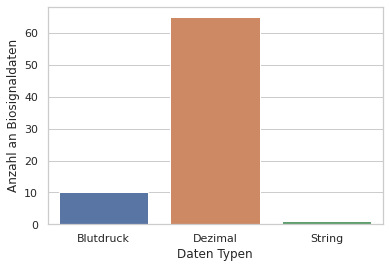
\includegraphics[height=8.5cm]{figures/biosignal_data_types}
	\caption[Datentypen der Biosignaldaten]{Datentypen der Biosignaldaten.}
	\label{fig:signaldatatyps}
\end{figure}

Auch die Distribution der Datenarten der \ac{fhir}-Profile ist zu berücksichtigen (\ref{fig:datenarten}). Die meist repräsentierte Datenart der Profile im Datensatz der Zuordnung ist die Art \glqq Parameter von Beatmung\grqq{} mit 36 zugeordneten Biosignaldaten. Diese Datenart ist auch die meist repräsentierte Art im Erweiterungsmodul \glqq Intensivmedizin\grqq{}.

\clearpage

\begin{figure}[ht]
	\centering
	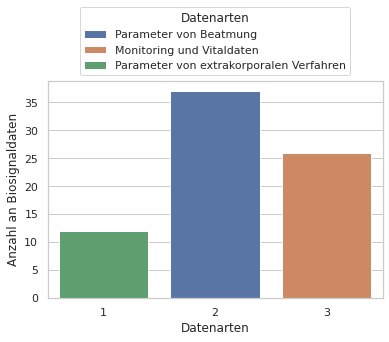
\includegraphics[height=8.5cm]{figures/datenarten}
	\caption[Datenarten der Profile]{Datenarten der Profile.}
	\label{fig:datenarten}
\end{figure}


	\section{\acs{fhir}-Profile} \label{sec:fhiricudisc}

Obwohl die \ac{fhir}-Profile des Moduls \glqq\ac{icu}\grqq{} für die Interoperabilität dienen sollten, beinhalten sie während der Durchführung dieses Projekts einige Irregularitäten, da sich das Modul in dieser Zeit in Abstimmung befindet, und weitere Untersuchungen und Tests von den \ac{mii}-Mitgliedern und anderen Benutzern erfolgen. So kam es vor, dass zwei \ac{fhir}-Profile im Erweiterungsmodul denselben Namen, aber spezifizieren unterschiedliche Beobachtungen beinhalten.

Die meisten definierten \ac{fhir}-Profile gehören zu der Kategorie \glqq Observation\grqq{} (\ref{tab:proficu}). Das liegt daran, dass das Ziel des Moduls die Spezifikationen der akutmedizinischen Daten ist, und gerade im Bereich der Intensivmedizin verlaufen die meisten Beobachtungen und Messungen (\glqq Observation\grqq{}).

Ein wichtiger Parameter für die Einhaltung der Interoperabilität im Gesundheitswesen sind die Codesysteme (\ref{tab:profilcodes}). Alle nicht generischen Profile beinhalten zumindest ein standardisiertes Codesystem. Die Profile der Kategorie \glqq Observation\grqq{} ohne Codesysteme gehören zu den generischen Profilen (\ref{fig:icutreegenerics}) und dienen der Modellierung der Daten (\ref{subsec:icumodul}). Aus diesem Grund beinhalten solche Profile keine Codesysteme und auch keine Maßeinheiten (\ref{tab:profilnocode}). Die Profile der Kategorie \glqq Procedure\grqq{} beinhalten auch keine Codesysteme, denn diese Profile speichern die Information der angewandten Geräte für die Durchführung eines Verfahrens und diese Information befindet sich im Basismodul \glqq Prozedur\grqq{} des Kerndatensatzes der \ac{mii}.

\begin{figure}[ht]
	\centering
	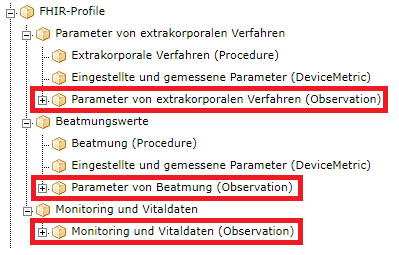
\includegraphics[height=8cm]{figures/icu_modul_tree_generics}
	\caption[Generische \glqq Observation\grqq{}-Profile]{Baumstruktur des Erweiterungsmoduls \glqq Intensivmedizin\grqq{}. Die generischen Profile der Kategorie \glqq Observation\grqq{} sind rot markiert.}
	\label{fig:icutreegenerics}
\end{figure}

Das Modul \glqq\ac{icu}\grqq{} ist das umfangreichste Modul der \ac{mii}. Von den Profilen dieses Moduls könnten in diesem Projekt 39 einem Biosignalparameter zugeordnet werden (\ref{fig:profile}). Die Gründe dieses Ergebnisses sind nicht nur von dem Umfang des Moduls abhängig, sondern von den Bioparameter im \ac{copra}-System (\ref{sec:configvarcopradiscu}).

\clearpage

\begin{figure}[ht]
	\centering
	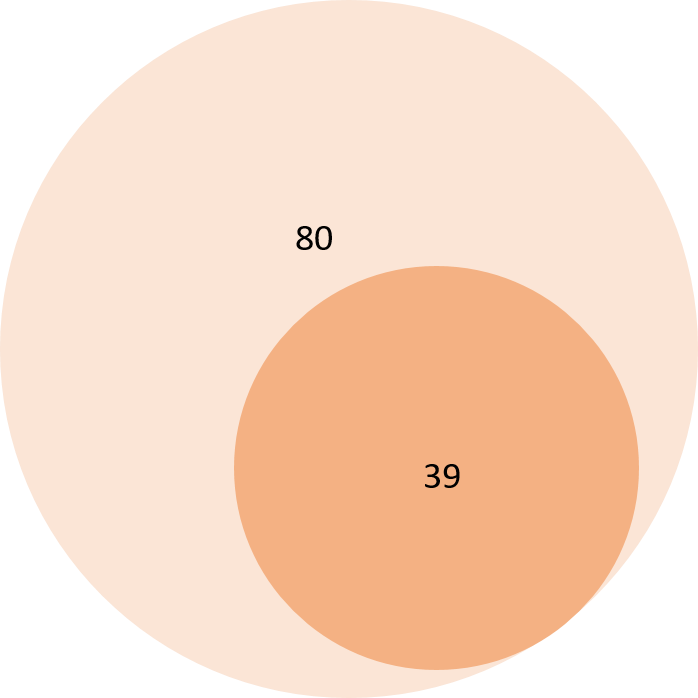
\includegraphics[height=7cm]{figures/profile}
	\caption[Diagramm der \acs{fhir}-Profile im Projekt]{Diagramm der \acs{fhir}-Profile im Projekt. Fast die Hälfte der \ac{fhir}-Profile konnten zugeordnet werden.}
	\label{fig:profile}
\end{figure}

	\section{Biosignaldaten aus \acs{copra}} \label{sec:configvarcopradiscu}

Die Daten aus \ac{copra} zeigten eine sehr geringe Interoperabilität. Ein Grund hierzu ist die fehlende Standardisierung bei der Schreibweise und Art der Maßeinheiten, da manche Einheiten und deren Darstellung nicht durch internationale etablierte Standards, wie die \ac{ucum} definiert sind. Das hat zufolge, dass die Maßeinheiten zwischen beiden Systemen harmonisiert werden müssen. Das hat zufolge, dass ein Teil der Information von \ac{copra} verloren geht. Für die Überführung der Daten aus \ac{copra} sollen die spezifizierten Einheiten der \ac{fhir}-Profile benutzt werden, denn die Maßeinheiten in den \ac{fhir}-Profilen sind durch standardisierte Codesysteme definiert.

Darüber hinaus sind manche Biosignaldaten im \ac{copra}-System nicht harmonisiert, denn das \ac{copra}-System beinhaltet keine der etablierten Codesysteme für die Codierung der Bioparameter. Das hat zufolge, dass in einigen Situationen dasselbe Biosignal von unterschiedlichen Geräten und/oder in diversen Stationen gemessen wird, aber unterschiedlich im System wahrgenommen wird. Ein Beispiel davon befindet sich in der  \ref{tab:sameprofilbiosig}.

\clearpage

 \begin{table}[ht]
 	\centering 
 	\caption[Dasselbe Biosignal gemessen durch zwei Geräte]{Dasselbe Biosignal gemessen durch zwei Geräte.}
 	\label{tab:sameprofilbiosig}
 	\begin{tabular}{|p{3.5cm}|p{2.4cm}|l|l|l|}
 		\hline
 		 \bfseries Profilname & \bfseries \ac{copra}-Name & \bfseries \acs{loinc} & \bfseries \ac{snomedct} & \bfseries Einheit \\ \hline
 		Beatmungsvolumen-Pro-Minute-Machineller-Beatmung & Beatmung \_MS\_Evita4 \_MV & 76009-0 & 426102006 & L/min \\ \hline
 		Beatmungsvolumen-Pro-Minute-Machineller-Beatmung & Beatmung \_MS\_Pallas \_MV & 76009-0 & 426102006 & L/min \\ \hline
 	\end{tabular}
 \end{table}

Nur eine der zugeordneten Biosignaldaten ist der Typ String (\ref{tab:stringvalue}). Durch andere Projekte, wie der \ac{aktin}-Notaufnahmeregister, wurde zur Kenntnis genommen, dass es weitere Biosignaldaten, wie die Pupillenweite oder Pupillenreaktion, auch der Datentyp String sind, und deren Informationen in den aktuellen \ac{copra}-Tabellen des Staging Bereichs des \ac{dw} sich befinden. Diese anderen Biosignalparameter können bei der Weiterentwicklung des Moduls \glqq Intensivmedizin\grqq{} betrachtet werden.

Andere erkannte Unregelmäßigkeiten sind die Namen und die Beschreibungen der Konfigurationsvariablen in \ac{copra}. Einerseits beinhalten viele Biosignaldaten keine Beschreibung für die Fachtermini im System, die die Daten dokumentieren. In dieser Situation befinden sich 379 der 701 relevanten Konfigurationsvariablen. Anderseits verfolgt die Benennung der Konfigurationsvariablen keine Standardnomenklatur, weder auf Deutsch noch auf Englisch. Aus diesem Grund wurden viele \ac{fhir}-Profile nicht gefunden. Aus diesem Grund ist viel Information verloren gegangen.

Einige Gründe für diese Problematiken sind zu einem die unterschiedlichen genutzten Geräte und zum anderen historische Hintergründe, da das \ac{copra}-System erst seit 2007 an der Universitätsmedizin Mainz etabliert und von verschiedenen Anwender und Anwenderinnen bedient wurde. Hinzukommend werden viele Daten im \ac{copra}-System manuell und nicht automatisiert eingetragen. Es gibt beispielsweise numerische Werte, die in Feldern für Freitexte gespeichert werden. Somit leidet die Qualität und Brauchbarkeit der Daten.

Einige \ac{fhir}-Profile wurden nicht gefunden, denn manche Beobachtungen oder Messungen am Standort Mainz werden im \ac{copra} nicht erfasst. Ein Beispiel davon ist das Profil \glqq Horowitz-In-Arteriellem-Blut\grqq{} in mm[Hg]. Stattdessen wird in \ac{copra} der Horowitz-Index ohne Einheit registriert.

Trotz dieser Hürden, konnten 70 Konfigurationsvariablen einem \ac{fhir}-Profil zugeordnet werden (\ref{fig:conf_var}). Die Ursachen dieses Ergebnisses liegen an den vorher genannten Problematiken und an der Komplexität und dem Umfang des Erweiterungsmoduls \glqq Intensivmedizin\grqq{}.

\begin{figure}[ht]
	\centering
	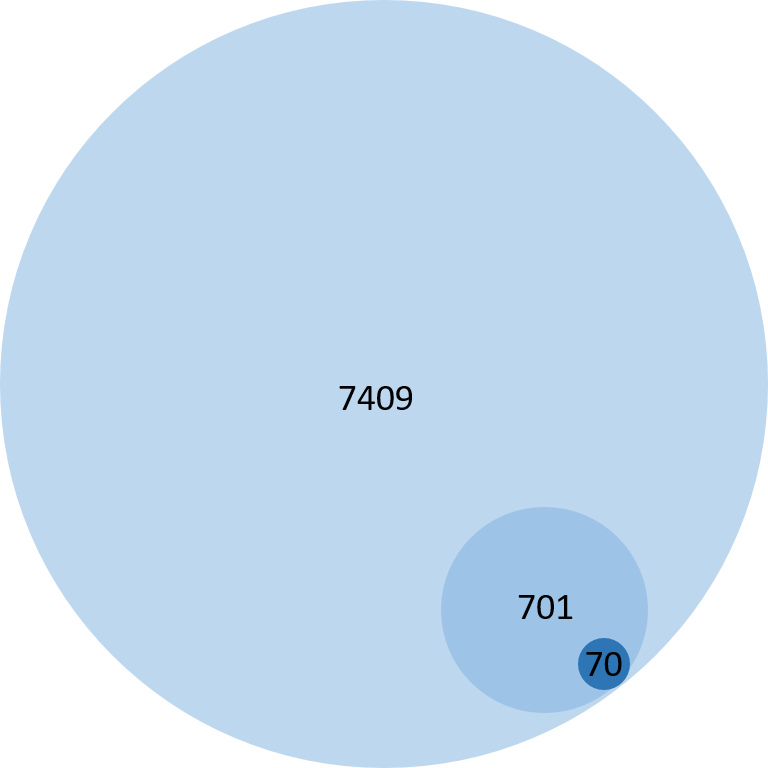
\includegraphics[height=7cm]{figures/config_var}
	\caption[Diagramm der Konfigurationsvariablen im Projekt]{Diagramm der Konfigurationsvariablen im Projekt. 70 der 701 relevanten Konfigurationsvariablen entsprechen einem Biosignalparameter, welches einem \ac{fhir}-Profil zugeordnet wurde. 
	}
	\label{fig:conf_var}
\end{figure}
	
	\chapter{Fazit und Ausblick} \label{ch:conclussion}

Mit der Zuordnung der gespeicherten Biosignaldaten aus dem \ac{pdms} mit den \ac{fhir}-Spezifikationen des Erweiterungsmoduls \glqq Intensivmedizin\grqq{} und die Bereitstellung dieser Daten für die Überführung in \ac{fhir} wurde das Ziel dieser Arbeit erreicht. Somit entstand ein Grundgerüst, welches für die Überführung der Biosignaldaten in \ac{fhir}-Ressource benutzt werden konnte. Diese Schritte sind entscheidend für die Gewährleistung der Interoperabilität der Biosignaldaten in \ac{copra}, und sind somit notwendige Komponenten der Datenmigration und Datenintegration.

Die Relevanz dieses Projekts liegt daran, dass die Biosignalparameter aus dem \ac{copra}-System der Universitätsmedizin Mainz mit Hilfe von der praktischen Umsetzung des Data Mappings in ein Standardformat überführt werden können. Das hat zufolge, dass diese Daten für Forschungszwecke weiterbenutzt werden können. Damit können die standardisierten Daten unter anderem für Datenauswertungen und Reports für Anwendungszwecke, Statistik, oder die Entwicklung von Systemen für die Unterstützung von klinischen Entscheidungen angewendet werden.

Ein weiterer wichtiger Aspekt dieses Projekts ist, dass mit der Überführung der Biosignaldaten in ein Standardformat mit standardisierten Codesystemen, die Daten am Ende auch die \ac{fair}-Prinzipien erhalten werden.

Dieses Projekt könnte auch der Grundstein für den Ideenaustausch und die Kooperation mit anderen \ac{mii}-Standorten werden.


	\newpage
	\addcontentsline{toc}{chapter}{Literatur}
	\nocite{*}           %  Die gesamte Literaturbibliothek wird eingefügt
	\printbibliography 
	
	\newpage	
	\begin{appendices}
	\clearpage
\renewcommand{\cleardoublepage}{}
\renewcommand{\clearpage}{}

\chapter{\acs{sql}} \label{sec:sql}

\acf{sql} ist die wichtigste nicht prozedurale Programmiersprache, um mit einem \ac{rdms} zu interagieren \cite{sqlpost}. Mit \ac{sql} werden die Struktur der Daten in einer \ac{db} definiert, modifiziert und Sicherheitsbedingungen aufgebaut \cite{dbsql}. \ac{sql} besitzt eine \ac{ddl} für die Beschreibung und Definition der \ac{db} und eine \ac{dml}, um die Daten in der \ac{db} zu manipulieren \cite{sqlpost, dbsql}.

\begin{itemize}
	\item \ac{ddl}-Befehle
	\begin{itemize}
		\item CREATE TABLE: Erzeugung einer Tabelle.
		\item DROP TABLE: Zum Löschen einer Tabelle.
		\item CREATE VIEW: Erzeugung einer View oder Sicht (virtuelle Tabelle).
		\item GRANT: Zum Gewähren von Zugriffsrechten.
	\end{itemize}
	\item \ac{dml}-Befehle
	\begin{itemize}
		\item SELECT: Abfragen.
		\item UPDATE: Änderung der Daten.
		\item DELETE: Löschung der Daten.
		\item INSERT: Zum Einfügen von Daten.
	\end{itemize}
\end{itemize}

\chapter{\acs{uri}, \acs{url} und \acs{urn}} \label{sec:uri}

Ein \acf{uri} ist eine Standardmethode für die Identifikation von Ressourcen in Internet, dieser Standard identifiziert die Ressourcen bei seiner Lokalisation, Name oder beides zusammen \cite{uribibdiff}. Das Schema eines \ac{uri} ist: \texttt{scheme://authority:/path?query\# fragment}, wobei \texttt{scheme} das Protokoll darstellt, z. B. \glqq \ac{http}\grqq{} \cite{uribibdiff, uribibdiff2}. \texttt{//authority} identifiziert die Domainadresse der Ressourcen und ist sogleich aus Benutzername, Host und Proxy aufgebaut \cite{uribibdiff, uribibdiff3}. \texttt{path} zeigt die komplette Adresse der Ressourcen zusammen mit einer Abfrage-Aktion (\texttt{?query}) \cite{uribibdiff2}. \texttt{fragment} ist ein Teil der referenzierten Ressourcen \cite{uribibdiff}.

 Ein \acf{url} ist die benutzte Zeichenkette, um die Ressourcen mit Hilfe von der Lokalisation zu erreichen, und ist somit ein Teil des \ac{uri} \cite{uribibdiff2}. Die Syntax eines \ac{url} ist: \texttt{scheme: subdomain/domain-na me. Top-level-domain/sub-folder}. Bei einem \ac{url}, genau wie bei dem \ac{uri}, liefert \texttt{scheme} die Details des Protokolls \cite{uribibdiff}. \texttt{subdomain} ist ein Teil der Domain, wie z. B. eine Facheinrichtung eines Krankenhauses. \texttt{domain-name} ist der Name der Domain, in dem vorherigen Beispiel der Name des Krankenhauses. \texttt{Top- level-domain} ist die Adresse der Domain im Internet, z. B. \glqq .de\grqq{} \cite{uribibdiff}. Das optionale Teil \texttt{sub-folder} definiert das Verzeichnis der Ressourcen \cite{uribibdiff, uribibdiff2}.
 
 Das \acf{urn}, genau wie das \ac{url}, gehört zu dem \ac{uri} \cite{uribibdiff}. Das \ac{urn} hat die folgende Syntax \texttt{urn:nid:nss} \cite{uribibdiff, uribibdiff2}. \texttt{urn} ist die Spezifikation des Schemas. \texttt{nid} ist der \glqq namespace identifier\grqq{} und definiert den Namensraum der Ressourcen \cite{uribibdiff}. Am Ende \texttt{nss} \glqq namespace-specific string\grqq{} ist der Namensraum der Ressourcen selbst \cite{uribibdiff}. Dieses Attribut ist optional \cite{uribibdiff2}. In einem \ac{urn} können mehre Folgen \texttt{nid:nss} vorkommen, wie urn:iso:std:iso:11073:10101 (\ref{subsec:ieee}).

 
 \chapter{Flussdiagramm} \label{sec:flowdiagram}
 
 Ein Flussdiagramm ist eines der am häufigsten verwendeten Diagramme. Es beschreibt und stellt einen Prozess, ein System oder einen Algorithmus dar. Flussdiagramme werden von technischen und nichttechnischen Personen in zahlreichen Bereichen verwendet, um komplexe Prozesse zu dokumentieren oder optimieren.
 
 Flussdiagramme werden mit zahlreichen Formen (\ref{fig:flowdiagramappen}) erstellt. Diese werden durch Verbindungspfeile vernetzt, um den Prozessfluss oder den Ablauf zu definieren.
 
 \begin{figure}[ht]
 	\centering
 	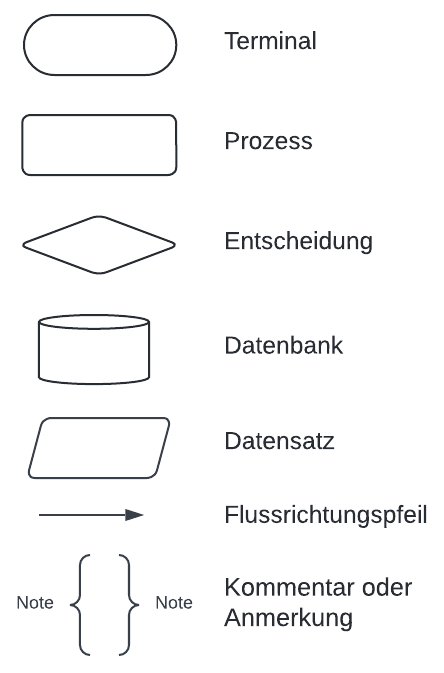
\includegraphics[height=6.5cm]{figures/flowdiagram}
 	\caption[Formen eines Flussdiagramms]{Formen eines Flussdiagramms.}
 	\label{fig:flowdiagramappen}
 \end{figure}

    \end{appendices}
	
	\newpage	
	\addcontentsline{toc}{chapter}{\listfigurename}
	\listoffigures
	
	\newpage	
	\addcontentsline{toc}{chapter}{\listtablename}
	\listoftables
	
	\newpage	
	\addcontentsline{toc}{chapter}{Listingverzeichnis}
	\lstlistoflistings
	
	\newpage	
	\addcontentsline{toc}{chapter}{Abkürzungsverzeichnis}
	\chapter*{Abkürzungsverzeichnis}

\begin{acronym}[ABK]
	\acro{aktin}[AKTIN]{Aktionsbündnis für Informations- und Kommunikationstechnologie in Intensiv- und Notfallmedizin}
	\acro{ansi}[ANSI]{American National Standards Institute}
	\acro{bmbf}[BMBF]{Bundesministerium für Bildung und Forschung}
	\acro{copra}[COPRA]{Computer Organized Patient Report Assistant}
	\acro{cpoe}[CPOE]{Computerized Physician Order Entry}
	\acro{csv}[CSV]{Comma-Separated Values}
	\acro{db}[DB]{Datenbank}
	\acro{dbms}[DBMS]{Datenbankmanagementsystem}
	\acro{ddl}[DDL]{Data Description Language}
	\acro{diz}[DIZ]{Datenintegrationszentrum}
	%\acro{dm}[DM]{Data Mart}
	\acro{dml}[DML]{Data Manipulation Language}
	\acro{drg}[DRG]{Diagnosis Related Group}
	\acro{dw}[DWH]{Data Warehouse}
	\acro{ecmo}[ECMO]{Extracorporaeal Membrane Oxigenation}
	\acro{edi}[EDI]{Electronic Data Interchange}
	\acro{ehr}[ePA]{elektronische Patienten Akte}
	\acro{etl}[ETL]{Extraction, Transformation, Load}
	\acro{fair}[FAIR]{Findable Accessible Interoperable Reusable}
	\acro{fhir}[FHIR]{Fast Healthcare Interoperability Resources}
	\acro{hl7}[HL7]{Health Level Seven}
	\acro{http}[HTTP]{Hypertext Transfer Protocol}
	\acro{icd}[ICD]{International Statistical Classification of Diseases and Related Health Problems}
	\acro{icu}[ICU]{Intensive Care Unit}
	\acro{ieee}[IEEE]{Institute of Electrical and Electronics Engineers}
	\acro{ihtsdo}[IHTSDO]{International Healthcare Terminology Standards Development Organization}
	\acro{iso}[ISO]{International Organization for Standardization}
	\acro{it}[IT]{Informationstechnik}
	\acro{json}[JSON]{JavaScript Object Notation}
	\acro{kis}[KIS]{Krankenhausinformationssystem}
	\acro{ldm}[LDM]{Logical Data Model}
	\acro{loinc}[LOINC]{Logical Observation Identifiers Names and Codes}
	\acro{lts}[LTS]{Long Term Support}
	\acro{mii}[MII]{Medizininformatik-Initiative}
	\acro{miracum}[MIRACUM]{Medical Informatics in Research and Care University Medicine}
	\acro{osi}[OSI]{Open Systems Interconnection}
	\acro{pdm}[PDM]{Physical Data Model}
	\acro{pdms}[PDMS]{Patientendatenmanagementsystem}
	\acro{rdms}[RDMS]{Relational Database Management System}
	\acro{refsets}[RefSets]{Referenz Sets}
	\acro{regex}[Regex]{Regular Expression}
	\acro{snomedct}[SNOMED CT]{Systematized Nomenclature of Medicine Clinical Terms}
	\acro{sql}[SQL]{Structued Query Language}
	\acro{xml}[XML]{Extensible Markup Language}
	\acro{xsd}[XSD]{Schema Definition Language}
	\acro{ucum}[UCUM]{Unified Code for Units of Measure}
	\acro{uri}[URI]{Uniform Resource Identifier}
	\acro{url}[URL]{Uniform Resource Locator}
	\acro{urn}[URN]{Uniform Resource Name}
	\acro{w3c}[W3C]{World Wide Web Consortium}
	\acro{who}[WHO]{Weltgesundheitsorganisation}

\end{acronym}


	
	\newpage	
	\addcontentsline{toc}{chapter}{Danksagung}
	\chapter*{Danksagung}

Quiero agradecer muy especialmente a las cuatro mujeres m\'as importantes en mi vida, Fefita, mi mam\'a, Sandrita y Mici por su amor, confianza y apoyo en todo momento.

Vielen Dank meinem Betreuer, Daniel Schmitz für die Hilfe bei der Realisierung dieses Projekts. Danke an Dr. Paul Schmücker für die Anmerkungen. Vielen Dank an Eric Schultheis, Thomas Schumacher und Petra Merle für die technische Unterstützung mit dem \acs{copra}-System. Vielen herzlichen Dank an Natalia Maier für die Revision und Korrektur dieser Mammutaufgabe und an Sami Habib für die Hilfe bei der Gestaltung der Präsentation. Besten Dank an Frau Jung für die ratsamen Wörter und Dr. Mathias Schwabe für die Ideen. Danke auch an alle die mich im Stich gelassen haben.
	
	
	\newpage	
    \pagestyle{empty} 
    \section*{Ehrenwörtliche Erklärung}

Ich versichere, dass ich die Masterarbeit selbständig verfasst und keine anderen als die angegebenen Quellen und Hilfsmittel benutzt habe. Ich habe die Masterarbeit in gleicher oder ähnlicher Form noch keiner anderen Prüfungsbehörde vorgelegt.

\vspace{1cm}
\noindent
\begin{tabular}{ p{0.5\textwidth} p{0.5\textwidth} }
	&       \hspace{0.5cm} \digsigfield{6cm}{2cm}{Unterschrift Hodelín Hernández Ehrenwörtliche Erklärung}         \\
	Mainz, den \today & Abel Hodelín Hernández
\end{tabular}

\vspace{2cm}

\section*{Erklärung zu Eigentum und Urheberrecht}

Hiermit erkläre ich mein Einverständnis, dass die  Hochschule Mannheim, die vorliegende Masterarbeit den Studierenden und interessierten Dritten zur Einsichtnahme zur Verfügung stellt und unter Nennung meines Namens (Urheber) veröffentlichen darf.

\vspace{1cm}
\noindent
\begin{tabular}{ p{0.5\textwidth} p{0.5\textwidth} }
	&       \hspace{0.5cm} \digsigfield{6cm}{2cm}{Unterschrift Hodelín Hernández Eigentum und Urheberrecht}         \\
	Mainz, den \today & Abel Hodelín Hernández
\end{tabular}

    
\end{document}
